%%%%%%%%%%%%%%%%%%%%%%%%%%%%%%%%%%%%%%%%%
% The Legrand Orange Book
% LaTeX Template
% Version 2.4 (26/09/2018)
%
% This template was downloaded from:
% http://www.LaTeXTemplates.com
%
% Original author:
% Mathias Legrand (legrand.mathias@gmail.com) with modifications by:
% Vel (vel@latextemplates.com)
%
% License:
% CC BY-NC-SA 3.0 (http://creativecommons.org/licenses/by-nc-sa/3.0/)
%
% Compiling this template:
% This template uses biber for its bibliography and makeindex for its index.
% When you first open the template, compile it from the command line with the 
% commands below to make sure your LaTeX distribution is configured correctly:
%
% 1) pdflatex main
% 2) makeindex main.idx -s StyleInd.ist
% 3) biber main
% 4) pdflatex main x 2
%
% After this, when you wish to update the bibliography/index use the appropriate
% command above and make sure to compile with pdflatex several times 
% afterwards to propagate your changes to the document.
%
% This template also uses a number of packages which may need to be
% updated to the newest versions for the template to compile. It is strongly
% recommended you update your LaTeX distribution if you have any
% compilation errors.
%
% Important note:
% Chapter heading images should have a 2:1 width:height ratio,
% e.g. 920px width and 460px height.
%
%%%%%%%%%%%%%%%%%%%%%%%%%%%%%%%%%%%%%%%%%

%----------------------------------------------------------------------------------------
%	PACKAGES AND OTHER DOCUMENT CONFIGURATIONS
%----------------------------------------------------------------------------------------
\documentclass[12pt]{book} % Default font size and left-justified equations
%\usepackage[toc,style=mcolindexgroup,nonumberlist,acronym,section=section]{glossaries}
\newcommand{\weblink}[1]{\textcolor{ocre}{\url{#1}}}
\newcommand{\weblinkT}[2]{\textcolor{ocre}{\href{#1}{#2}}}
\usepackage{glossaries}
%\usepackage[counter=page,xindy,section=page]{glossaries}
%\usepackage{datatool-base} %used for glossaries
\usepackage[export]{adjustbox} %for adjusting figure alignment
\usepackage[
  text={7in,10in},
  centering
]{geometry}
\usepackage{tikz}
\usetikzlibrary{arrows.meta, positioning, calc, matrix, shapes}
\usepackage{pstricks}
\usepackage{pst-barcode}
\usepackage{floatrow}
\usepackage{amsmath}
\usepackage{booktabs} % For nicer table formatting
\usepackage{array}    % For more control over column width
\usepackage{colortbl}%color background in tables
\usepackage{pgfplots}
\usepgfplotslibrary{fillbetween}
\usepgfplotslibrary{groupplots}
\usepackage{wrapfig}
\usepackage{xcolor, soul}
\usepackage{listings}
\usepackage[most]{tcolorbox}
\tcbuselibrary{listingsutf8,listings, skins} % Allows for listings support in tcolorbox\tcbuselibrary{listings, skins}
\renewcommand*{\glstextformat}{\textbf}
\usetikzlibrary{shadows}
\sethlcolor{gray!5}
\usepackage{shadowtext}
\usepackage{caption}%needed to change caption alignment
\captionsetup{justification=raggedright,singlelinecheck=false}
\usepackage{fancyvrb} %fancy Verbatim stuff
\usepackage{placeins} %dealing with floats like wrapfig
\usepackage{enumitem}
\usepackage[utf8]{inputenc}
\usepackage{parcolumns}
\usepackage{hyperref}
\usepackage{graphicx}
\usepackage{lmodern}

\newcommand*{\button}[1]{\colorbox{gray!40}{\shadowtext{#1}}}

%Chapter-specific Glossaries
\newglossary[tlg]{datacollection}{tld}{tdn}{Glossary of Terms}

\newglossary[tlg]{graphtheory}{tld}{tdn}{Glossary of Terms}

%codeblock counter
\newcounter{codeblock}[chapter]
\newenvironment{codeblock}[1][]{\refstepcounter{codeblock}\par\medskip
   \textbf{Code block~\thechapter.\thecodeblock #1} \rmfamily}{\medskip}

%Two-column glossary style
\newglossarystyle{twocolumn}{
\setglossarystyle{list}% base this style on the list style
\renewenvironment{theglossary}{
\begin{multicols}{2}\begin{description}}{\end{description}\end{multicols}} 
% the default environment for list is \begin{description} \end{description}
} 
%GLOSSARY TERMS
\newglossaryentry{transduction}{name={transduction},description={The conversion of physical energy (light, sound, etc.) to action potentials}}
%-----------------------------------------------
%        Data Collection Glossary
%-----------------------------------------------
\newglossaryentry{open source software}{
type={datacollection},
name={Open Source Software},
text={open source software},
description={Open source software is software with source code that anyone can inspect, modify, and enhance.}}

\newglossaryentry{polling rate}{type={datacollection}, name={Polling Rate},
text={polling rate},description={The rate at which the status of a peripheral input to a computer like a keyboard or mouse is checked.}}

\newglossaryentry{measurement error}{type={datacollection}, name={Measurement error},text={measurement error},description={Measurement Error is the difference between a measured quantity and its true value. Measurement error can be due to random errors of measurement or systematic errors such as a mis-calibrated measurement instrument.}}

\newglossaryentry{URL}{type={datacollection}, name={URL},description={A Uniform Resource Locator (URL), colloquially termed a web address,[1] is a reference to a web resource that specifies its location on a computer network and a mechanism for retrieving it.}}

\newglossaryentry{web hosting service}{
    type={datacollection}, 
    name={Web hosting service},
    text={web hosting service},
    description={A web hosting service is a type of Internet hosting service that allows individuals and organizations to make their website accessible via the World Wide Web. Web hosts are companies that provide space on a server owned or leased for use by clients, as well as providing Internet connectivity, typically in a data center.}}
 
\newglossaryentry{platform independent}{
    type={datacollection},
    name={Platform independent},
    text={platform independent},
    description={describes software that does not depend on a specific operating system like Windows MacOSx, or Linux.}
}

\newglossaryentry{Compile}{
    type={datacollection},
    name={Compile},
    text={compile},
    description={Convert a program or script into machine-code or lower-level form in which the program can be executed by a computer.}
}

\newglossaryentry{principal investigator}{
    type={datacollection},
    name={Principal Investigator (PI)},
    text={principal investigator},
    description={The lead researcher for a grant project, laboratory study, or a clinical trial. The phrase is also often used as a synonym for ``head of the laboratory" or ``research group leader".}
}

\newglossaryentry{aggregate data}{
    type={datacollection},
    name={Aggregate Data},
    text={aggregate data},
    description={High-level data which is acquired by combining individual-level data.}
}

\newglossaryentry{task schematic}{
    type={datacollection},
    name={Task Schematic},
    text={task schematic},
    description={A figure depicting the major components, sequence and, and timing of an experimental task.}
}

\newglossaryentry{inter-stimulus interval}{
    type={datacollection},
    name={Inter-stimulus Interval (ISI)},
    text={inter-stimulus interval},
    description={The interval of time between the offset of one stimulus and the onset of the next stimulus in an experiment.}
}

\newglossaryentry{inter-trial interval}{
    type={datacollection},
    name={Inter-trial Interval (ITI)},
    text={inter-trial interval},
    description={The interval of time between the offset of a stimulus marking the end of an trial and the onset of a stimulus marking the beginning of the next trial in an experiment.}
}

\newglossaryentry{extraneous variables}{
    type={datacollection},
    name={Extraneous variable},
    text={Extraneous Variable},
    description={Extraneous variables are all variables, which are not the independent variable, but could affect the results of the experiment.}
}

\newglossaryentry{variable}{
    type={datacollection},
    name={Variable},
    text={variable},
    description={Variables in programming are like containers that hold information for later reference or manipulation. Their purpose is to label and store data.}
}

\newglossaryentry{conditional execution}{
    type={datacollection},
    name={Conditional Execution},
    text={conditional execution},
    description={When one or more instruction(s) are executed only when a specific test condition is determined to be true.}
}

\newglossaryentry{informed consent}{
    type={datacollection},
    name={Informed Consent},
    text={informed consent},
    description={Informed consent is a process for getting permission from participants before conducting an intervention conducting any form of research on a person, or for disclosing a person's information.}
}

\newglossaryentry{local variable}{
    type={datacollection},
    name={Local Variable},
    text={local variable},
    description={In computer science, a local variable is one that is defined in a function or block and that is available only in that function or block. It is not accessible outside the block.}
}

\newglossaryentry{global variable}{
    type={datacollection},
    name={Global Variable},
    text={global variable},
    description={A variable whose value is accessible from inside any function or block.}
}


%-----------------------------------------------------------------------------------
%.    GRAPH THEORY
%----------------------------------------------------------------------------------

\newglossaryentry{undirected graphs}{
    type={graphtheory},
    name={Undirected Graphs},
    text={undirected graphs},
    description={A graph with bidirectional relationships.}
}

\newglossaryentry{Directed graphs}{
    type={graphtheory},
    name={Directed Graphs},
    text={Directed graphs},
    description={A graph with unidirectional relationships.}
}

\newglossaryentry{Degree}{
    type={graphtheory},
    name={Degree},
    text={Degree},
    description={A fundamental graph metric that counts the number of edges connected to a node. In the example graph, each node has degree 2, meaning it connects to exactly two other nodes in the hexagonal arrangement. For directed graphs, degree can be split into in-degree (incoming connections) and out-degree (outgoing connections).}
}

\newglossaryentry{centrality}{
    type={graphtheory},
    name={Centrality},
    text={centrality},
    description={A fundamental graph metric that counts the number of edges connected to a node. In the example graph, each node has degree 2, meaning it connects to exactly two other nodes in the hexagonal arrangement. For directed graphs, degree can be split into in-degree (incoming connections) and out-degree (outgoing connections).A measure of a node's importance or influence within a network.}
}

\newglossaryentry{clustering coefficient}{
    type={graphtheory},
    name={Clustering Coefficient},
    text={clustering coefficient},
    description={A measure of the degree to which nodes in a graph tend to cluster together, quantifying how close a node's neighbors are to being a complete graph.}
}

\makeglossaries

\raggedbottom

%%%%%%%%%%%%%%%%%%%%%%%%%%%%%%%%%%%%%%%%%
% The Legrand Orange Book
% Structural Definitions File
% Version 2.1 (26/09/2018)
%
% Original author:
% Mathias Legrand (legrand.mathias@gmail.com) with modifications by:
% Vel (vel@latextemplates.com)
% 
% This file was downloaded from:
% http://www.LaTeXTemplates.com
%
% License:
% CC BY-NC-SA 3.0 (http://creativecommons.org/licenses/by-nc-sa/3.0/)
%
%%%%%%%%%%%%%%%%%%%%%%%%%%%%%%%%%%%%%%%%%

%----------------------------------------------------------------------------------------
%	VARIOUS REQUIRED PACKAGES AND CONFIGURATIONS
%----------------------------------------------------------------------------------------
\usepackage{graphicx} % Required for including pictures
\graphicspath{{Pictures/}} % Specifies the directory where pictures are stored

\usepackage{lipsum} % Inserts dummy text

\usepackage{tikz} % Required for drawing custom shapes

\usepackage[english]{babel} % English language/hyphenation

\usepackage{enumitem} % Customize lists
\setlist{nolistsep} % Reduce spacing between bullet points and numbered lists

\usepackage{booktabs} % Required for nicer horizontal rules in tables

\usepackage{xcolor} % Required for specifying colors by name
\definecolor{ocre}{RGB}{0,0,100} % Define the orange color used for highlighting throughout the book

\usepackage{hyperref}
\usepackage{epigraph}%Used for chapter quotes
\usepackage{minitoc} % Table of contents for Chapters

%----------------------------------------------------------------------------------------
%	MARGINS
%----------------------------------------------------------------------------------------

\usepackage{geometry} % Required for adjusting page dimensions and margins

\geometry{
	paper=letterpaper, % Paper size, change to letterpaper for US letter size
	top=2cm, % Top margin
	bottom=2cm, % Bottom margin
	left=2cm, % Left margin
	right=2cm, % Right margin
	headheight=14.49998pt, % Header height
	footskip=1.4cm, % Space from the bottom margin to the baseline of the footer
	headsep=10pt, % Space from the top margin to the baseline of the header
	%showframe, % Uncomment to show how the type block is set on the page
}

%----------------------------------------------------------------------------------------
%	Chapter Glossaries 

%----------------------------------------------------------------------------------------
%\newglossarystyle{chapterglossary}%
%{%
%  \setglossarystyle{list}%
%  \renewcommand*{\glossaryentrynumbers}[1]{\striprelax##1\endstripre%lax{}}%
%  \renewcommand*{\glsXchapterXglsnumberformat}[2]{##2}%
%  \renewcommand*{\delimR}{,}%
%  \renewcommand*{\glossentry}[2]{%
%    \edef\doifinlocation{\noexpand\ifinlocation{\thechapter}{##2}}%
%    \doifinlocation
%    {%
%      \item \glossentryname{##1} \glossentrydesc{##1}%
%    }%
%  }%
%}
%\newcommand{\ifinlocation}[3]{%
% \DTLifinlist{#1}{#2}{#3}{}%
%}
%\def\striprelax\relax#1\endstriprelax{#1}
%\setglossarystyle{chapterglossary}
%----------------------------------------------------------------------------------------
%	FONTS
%----------------------------------------------------------------------------------------

\usepackage{avant} % Use the Avantgarde font for headings
%\usepackage{times} % Use the Times font for headings
\usepackage{mathptmx} % Use the Adobe Times Roman as the default text font together with math symbols from the Sym­bol, Chancery and Com­puter Modern fonts

\usepackage{microtype} % Slightly tweak font spacing for aesthetics
\usepackage[utf8]{inputenc} % Required for including letters with accents
\usepackage[T1]{fontenc} % Use 8-bit encoding that has 256 glyphs

%----------------------------------------------------------------------------------------
%	BIBLIOGRAPHY AND INDEX
%----------------------------------------------------------------------------------------
 
\usepackage[sectionbib]{natbib}
\usepackage{chapterbib}
\renewcommand{\bibname}{References} %use "References"

%%\usepackage[style=numeric,citestyle=numeric,sorting=nyt,sortcites=true,autopunct=true,autolang=hyphen,abbreviate=false,backend=biber]{biblatex}
%%\addbibresource{bibliography.bib} % BibTeX bibliography file
%%\defbibheading{bibempty}{}


\usepackage{calc} % For simpler calculation - used for spacing the index letter headings correctly
\usepackage{makeidx} % Required to make an index
\makeindex % Tells LaTeX to create the files required for indexing

%----------------------------------------------------------------------------------------
%	MAIN TABLE OF CONTENTS
%----------------------------------------------------------------------------------------

\usepackage{titletoc} % Required for manipulating the table of contents

\contentsmargin{0cm} % Removes the default margin

% Part text styling (this is mostly taken care of in the PART HEADINGS section of this file)
\titlecontents{part}
	[0cm] % Left indentation
	{\addvspace{20pt}\bfseries} % Spacing and font options for parts
	{}
	{}
	{}

% Chapter text styling
\titlecontents{chapter}
	[1.25cm] % Left indentation
	{\addvspace{12pt}\large\sffamily\bfseries} % Spacing and font options for chapters
	{\color{ocre!60}\contentslabel[\Large\thecontentslabel]{1.25cm}\color{ocre}} % Formatting of numbered sections of this type
	{\color{ocre}} % Formatting of numberless sections of this type
	{\color{ocre!60}\normalsize\;\titlerule*[.5pc]{.}\;\thecontentspage} % Formatting of the filler to the right of the heading and the page number

% Section text styling
\titlecontents{section}
	[1.25cm] % Left indentation
	{\addvspace{3pt}\sffamily\bfseries} % Spacing and font options for sections
	{\contentslabel[\thecontentslabel]{1.25cm}} % Formatting of numbered sections of this type
	{} % Formatting of numberless sections of this type
	{\hfill\color{black}\thecontentspage} % Formatting of the filler to the right of the heading and the page number

% Subsection text styling
\titlecontents{subsection}
	[1.25cm] % Left indentation
	{\addvspace{1pt}\sffamily\small} % Spacing and font options for subsections
	{\contentslabel[\thecontentslabel]{1.25cm}} % Formatting of numbered sections of this type
	{} % Formatting of numberless sections of this type
	{\ \titlerule*[.5pc]{.}\;\thecontentspage} % Formatting of the filler to the right of the heading and the page number

% Figure text styling
\titlecontents{figure}
	[1.25cm] % Left indentation
	{\addvspace{1pt}\sffamily\small} % Spacing and font options for figures
	{\thecontentslabel\hspace*{1em}} % Formatting of numbered sections of this type
	{} % Formatting of numberless sections of this type
	{\ \titlerule*[.5pc]{.}\;\thecontentspage} % Formatting of the filler to the right of the heading and the page number

% Table text styling
\titlecontents{table}
	[1.25cm] % Left indentation
	{\addvspace{1pt}\sffamily\small} % Spacing and font options for tables
	{\thecontentslabel\hspace*{1em}} % Formatting of numbered sections of this type
	{} % Formatting of numberless sections of this type
	{\ \titlerule*[.5pc]{.}\;\thecontentspage} % Formatting of the filler to the right of the heading and the page number

%----------------------------------------------------------------------------------------
%	MINI TABLE OF CONTENTS IN PART HEADS
%----------------------------------------------------------------------------------------

% Chapter text styling
\titlecontents{lchapter}
	[0em] % Left indentation
	{\addvspace{15pt}\large\sffamily\bfseries} % Spacing and font options for chapters
	{\color{ocre}\contentslabel[\Large\thecontentslabel]{1.25cm}\color{ocre}} % Chapter number
	{}  
	{\color{ocre}\normalsize\sffamily\bfseries\;\titlerule*[.5pc]{.}\;\thecontentspage} % Page number

% Section text styling
\titlecontents{lsection}
	[0em] % Left indentation
	{\sffamily\small} % Spacing and font options for sections
	{\contentslabel[\thecontentslabel]{1.25cm}} % Section number
	{}
	{}

% Subsection text styling (note these aren't shown by default, display them by searchings this file for tocdepth and reading the commented text)
\titlecontents{lsubsection}
	[.5em] % Left indentation
	{\sffamily\footnotesize} % Spacing and font options for subsections
	{\contentslabel[\thecontentslabel]{1.25cm}}
	{}
	{}

%----------------------------------------------------------------------------------------
%	HEADERS AND FOOTERS
%----------------------------------------------------------------------------------------

\usepackage{fancyhdr} % Required for header and footer configuration

\pagestyle{fancy} % Enable the custom headers and footers

\renewcommand{\chaptermark}[1]{\markboth{\sffamily\normalsize\bfseries\chaptername\ \thechapter.\ #1}{}} % Styling for the current chapter in the header
\renewcommand{\sectionmark}[1]{\markright{\sffamily\normalsize\thesection\hspace{5pt}#1}{}} % Styling for the current section in the header

\fancyhf{} % Clear default headers and footers
\fancyhead[LE,RO]{\sffamily\normalsize\thepage} % Styling for the page number in the header
\fancyhead[LO]{\rightmark} % Print the nearest section name on the left side of odd pages
\fancyhead[RE]{\leftmark} % Print the current chapter name on the right side of even pages
%\fancyfoot[C]{\thepage} % Uncomment to include a footer

\renewcommand{\headrulewidth}{0.5pt} % Thickness of the rule under the header

\fancypagestyle{plain}{% Style for when a plain pagestyle is specified
	\fancyhead{}\renewcommand{\headrulewidth}{0pt}%
}

% Removes the header from odd empty pages at the end of chapters
\makeatletter
\renewcommand{\cleardoublepage}{
\clearpage\ifodd\c@page\else
\hbox{}
\vspace*{\fill}
\thispagestyle{empty}
\newpage
\fi}

%----------------------------------------------------------------------------------------
%	THEOREM STYLES
%----------------------------------------------------------------------------------------

\usepackage{amsmath,amsfonts,amssymb,amsthm} % For math equations, theorems, symbols, etc

\newcommand{\intoo}[2]{\mathopen{]}#1\,;#2\mathclose{[}}
\newcommand{\ud}{\mathop{\mathrm{{}d}}\mathopen{}}
\newcommand{\intff}[2]{\mathopen{[}#1\,;#2\mathclose{]}}
\renewcommand{\qedsymbol}{$\blacksquare$}
\newtheorem{notation}{Notation}[chapter]

% Boxed/framed environments
\newtheoremstyle{ocrenumbox}% Theorem style name
{0pt}% Space above
{0pt}% Space below
{\normalfont}% Body font
{}% Indent amount
{\small\bf\sffamily\color{ocre}}% Theorem head font
{\;}% Punctuation after theorem head
{0.25em}% Space after theorem head
{\small\sffamily\color{ocre}\thmname{#1}\nobreakspace\thmnumber{\@ifnotempty{#1}{}\@upn{#2}}% Theorem text (e.g. Theorem 2.1)
\thmnote{\nobreakspace\the\thm@notefont\sffamily\bfseries\color{black}---\nobreakspace#3.}} % Optional theorem note

\newtheoremstyle{blacknumex}% Theorem style name
{5pt}% Space above
{5pt}% Space below
{\normalfont}% Body font
{} % Indent amount
{\small\bf\sffamily}% Theorem head font
{\;}% Punctuation after theorem head
{0.25em}% Space after theorem head
{\small\sffamily{\tiny\ensuremath{\blacksquare}}\nobreakspace\thmname{#1}\nobreakspace\thmnumber{\@ifnotempty{#1}{}\@upn{#2}}% Theorem text (e.g. Theorem 2.1)
\thmnote{\nobreakspace\the\thm@notefont\sffamily\bfseries---\nobreakspace#3.}}% Optional theorem note

\newtheoremstyle{blacknumbox} % Theorem style name
{0pt}% Space above
{0pt}% Space below
{\normalfont}% Body font
{}% Indent amount
{\small\bf\sffamily}% Theorem head font
{\;}% Punctuation after theorem head
{0.25em}% Space after theorem head
{\small\sffamily\thmname{#1}\nobreakspace\thmnumber{\@ifnotempty{#1}{}\@upn{#2}}% Theorem text (e.g. Theorem 2.1)
\thmnote{\nobreakspace\the\thm@notefont\sffamily\bfseries---\nobreakspace#3.}}% Optional theorem note

% Non-boxed/non-framed environments
\newtheoremstyle{ocrenum}% Theorem style name
{5pt}% Space above
{5pt}% Space below
{\normalfont}% Body font
{}% Indent amount
{\small\bf\sffamily\color{ocre}}% Theorem head font
{\;}% Punctuation after theorem head
{0.25em}% Space after theorem head
{\small\sffamily\color{ocre}\thmname{#1}\nobreakspace\thmnumber{\@ifnotempty{#1}{}\@upn{#2}}% Theorem text (e.g. Theorem 2.1)
\thmnote{\nobreakspace\the\thm@notefont\sffamily\bfseries\color{black}---\nobreakspace#3.}} % Optional theorem note
\makeatother

% Defines the theorem text style for each type of theorem to one of the three styles above
\newcounter{dummy} 
\numberwithin{dummy}{section}
\theoremstyle{ocrenumbox}
\newtheorem{theoremeT}[dummy]{Theorem}
\newtheorem{problem}{Problem}[chapter]
\newtheorem{exerciseT}{Exercise}[chapter]
\theoremstyle{blacknumex}
\newtheorem{exampleT}{Example}[chapter]
\theoremstyle{blacknumbox}
\newtheorem{vocabulary}{Vocabulary}[chapter]
\newtheorem{definitionT}{Definition}[section]
\newtheorem{corollaryT}[dummy]{Links to Learning}
\theoremstyle{ocrenum}
\newtheorem{proposition}[dummy]{Proposition}

%----------------------------------------------------------------------------------------
%	DEFINITION OF COLORED BOXES
%----------------------------------------------------------------------------------------

\RequirePackage[framemethod=default]{mdframed} % Required for creating the theorem, definition, exercise and corollary boxes

% Theorem box
\newmdenv[skipabove=7pt,
skipbelow=7pt,
backgroundcolor=black!5,
linecolor=ocre,
innerleftmargin=5pt,
innerrightmargin=5pt,
innertopmargin=5pt,
leftmargin=0cm,
rightmargin=0cm,
innerbottommargin=5pt]{tBox}

% Exercise box	  
\newmdenv[skipabove=7pt,
skipbelow=7pt,
rightline=false,
leftline=true,
topline=false,
bottomline=false,
backgroundcolor=ocre!10,
linecolor=ocre,
innerleftmargin=5pt,
innerrightmargin=5pt,
innertopmargin=5pt,
innerbottommargin=5pt,
leftmargin=0cm,
rightmargin=0cm,
linewidth=4pt]{eBox}	

% Definition box
\newmdenv[skipabove=7pt,
skipbelow=7pt,
rightline=false,
leftline=true,
topline=false,
bottomline=false,
linecolor=ocre,
innerleftmargin=5pt,
innerrightmargin=5pt,
innertopmargin=0pt,
leftmargin=0cm,
rightmargin=0cm,
linewidth=4pt,
innerbottommargin=0pt]{dBox}	

% Corollary box
\newmdenv[skipabove=7pt,
skipbelow=7pt,
rightline=false,
leftline=true,
topline=false,
bottomline=false,
linecolor=gray,
backgroundcolor=green!15,
innerleftmargin=5pt,
innerrightmargin=5pt,
innertopmargin=5pt,
leftmargin=0cm,
rightmargin=0cm,
linewidth=4pt,
innerbottommargin=5pt]{cBox}

% Creates an environment for each type of theorem and assigns it a theorem text style from the "Theorem Styles" section above and a colored box from above
\newenvironment{theorem}{\begin{tBox}\begin{theoremeT}}{\end{theoremeT}\end{tBox}}
\newenvironment{exercise}{\begin{eBox}\begin{exerciseT}}{\hfill{\color{ocre}\tiny\ensuremath{\blacksquare}}\end{exerciseT}\end{eBox}}				  
\newenvironment{definition}{\begin{dBox}\begin{definitionT}}{\end{definitionT}\end{dBox}}	
\newenvironment{example}{\begin{exampleT}}{\hfill{\tiny\ensuremath{\blacksquare}}\end{exampleT}}		
\newenvironment{corollary}{\begin{cBox}\begin{corollaryT}}{\end{corollaryT}\end{cBox}}	

%----------------------------------------------------------------------------------------
%	REMARK ENVIRONMENT
%----------------------------------------------------------------------------------------

\newenvironment{remark}{\par\vspace{10pt}\small % Vertical white space above the remark and smaller font size
\begin{list}{}{
\leftmargin=35pt % Indentation on the left
\rightmargin=25pt}\item\ignorespaces % Indentation on the right
\makebox[-2.5pt]{\begin{tikzpicture}[overlay]
\node[draw=ocre!60,line width=1pt,circle,fill=ocre!25,font=\sffamily\bfseries,inner sep=2pt,outer sep=0pt] at (-15pt,0pt){\textcolor{ocre}{R}};\end{tikzpicture}} % Orange R in a circle
\advance\baselineskip -1pt}{\end{list}\vskip5pt} % Tighter line spacing and white space after remark

%----------------------------------------------------------------------------------------
%	SECTION NUMBERING IN THE MARGIN
%----------------------------------------------------------------------------------------

\makeatletter
\renewcommand{\@seccntformat}[1]{\llap{\textcolor{ocre}{\csname the#1\endcsname}\hspace{1em}}}                    
\renewcommand{\section}{\@startsection{section}{1}{\z@}
{-4ex \@plus -1ex \@minus -.4ex}
{1ex \@plus.2ex }
{\normalfont\large\sffamily\bfseries}}
\renewcommand{\subsection}{\@startsection {subsection}{2}{\z@}
{-3ex \@plus -0.1ex \@minus -.4ex}
{0.5ex \@plus.2ex }
{\normalfont\sffamily\bfseries}}
\renewcommand{\subsubsection}{\@startsection {subsubsection}{3}{\z@}
{-2ex \@plus -0.1ex \@minus -.2ex}
{.2ex \@plus.2ex }
{\normalfont\small\sffamily\bfseries}}                        
\renewcommand\paragraph{\@startsection{paragraph}{4}{\z@}
{-2ex \@plus-.2ex \@minus .2ex}
{.1ex}
{\normalfont\small\sffamily\bfseries}}

%----------------------------------------------------------------------------------------
%	PART HEADINGS
%----------------------------------------------------------------------------------------

% Numbered part in the table of contents
\newcommand{\@mypartnumtocformat}[2]{%
	\setlength\fboxsep{0pt}%
	\noindent\colorbox{ocre!20}{\strut\parbox[c][.7cm]{\ecart}{\color{ocre!70}\Large\sffamily\bfseries\centering#1}}\hskip\esp\colorbox{ocre!40}{\strut\parbox[c][.7cm]{\linewidth-\ecart-\esp}{\Large\sffamily\centering#2}}%
}

% Unnumbered part in the table of contents
\newcommand{\@myparttocformat}[1]{%
	\setlength\fboxsep{0pt}%
	\noindent\colorbox{ocre!40}{\strut\parbox[c][.7cm]{\linewidth}{\Large\sffamily\centering#1}}%
}

\newlength\esp
\setlength\esp{4pt}
\newlength\ecart
\setlength\ecart{1.2cm-\esp}
\newcommand{\thepartimage}{}%
\newcommand{\partimage}[1]{\renewcommand{\thepartimage}{#1}}%
\def\@part[#1]#2{%
\ifnum \c@secnumdepth >-2\relax%
\refstepcounter{part}%
\addcontentsline{toc}{part}{\texorpdfstring{\protect\@mypartnumtocformat{\thepart}{#1}}{\partname~\thepart\ ---\ #1}}
\else%
\addcontentsline{toc}{part}{\texorpdfstring{\protect\@myparttocformat{#1}}{#1}}%
\fi%
\startcontents%
\markboth{}{}%
{\thispagestyle{empty}%
\begin{tikzpicture}[remember picture,overlay]%
\node at (current page.north west){\begin{tikzpicture}[remember picture,overlay]%	
\fill[ocre!20](0cm,0cm) rectangle (\paperwidth,-\paperheight);
\node[anchor=north] at (4cm,-3.25cm){\color{ocre!40}\fontsize{220}{100}\sffamily\bfseries\thepart}; 
\node[anchor=south east] at (\paperwidth-1cm,-\paperheight+1cm){\parbox[t][][t]{8.5cm}{
\printcontents{l}{0}{\setcounter{tocdepth}{1}}% The depth to which the Part mini table of contents displays headings; 0 for chapters only, 1 for chapters and sections and 2 for chapters, sections and subsections
}};
\node[anchor=north east] at (\paperwidth-1.5cm,-3.25cm){\parbox[t][][t]{15cm}{\strut\raggedleft\color{white}\fontsize{30}{30}\sffamily\bfseries#2}};
\end{tikzpicture}};
\end{tikzpicture}}%
\@endpart}
\def\@spart#1{%
\startcontents%
\phantomsection
{\thispagestyle{empty}%
\begin{tikzpicture}[remember picture,overlay]%
\node at (current page.north west){\begin{tikzpicture}[remember picture,overlay]%	
\fill[ocre!20](0cm,0cm) rectangle (\paperwidth,-\paperheight);
\node[anchor=north east] at (\paperwidth-1.5cm,-3.25cm){\parbox[t][][t]{15cm}{\strut\raggedleft\color{white}\fontsize{30}{30}\sffamily\bfseries#1}};
\end{tikzpicture}};
\end{tikzpicture}}
\addcontentsline{toc}{part}{\texorpdfstring{%
\setlength\fboxsep{0pt}%
\noindent\protect\colorbox{ocre!40}{\strut\protect\parbox[c][.7cm]{\linewidth}{\Large\sffamily\protect\centering #1\quad\mbox{}}}}{#1}}%
\@endpart}
\def\@endpart{\vfil\newpage
\if@twoside
\if@openright
\null
\thispagestyle{empty}%
\newpage
\fi
\fi
\if@tempswa
\twocolumn
\fi}

%----------------------------------------------------------------------------------------
%	CHAPTER HEADINGS
%----------------------------------------------------------------------------------------

% A switch to conditionally include a picture, implemented by Christian Hupfer
\newif\ifusechapterimage
\usechapterimagetrue
\newcommand{\thechapterimage}{}%
\newcommand{\chapterimage}[1]{\ifusechapterimage\renewcommand{\thechapterimage}{#1}\fi}%
\newcommand{\autodot}{.}
\def\@makechapterhead#1{%
{\parindent \z@ \raggedright \normalfont
\ifnum \c@secnumdepth >\m@ne
\if@mainmatter
\begin{tikzpicture}[remember picture,overlay]
\node at (current page.north west)
{\begin{tikzpicture}[remember picture,overlay]
\node[anchor=north west,inner sep=0pt] at (0,0) {\ifusechapterimage\includegraphics[width=\paperwidth]{\thechapterimage}\fi};
\draw[anchor=west] (\Gm@lmargin,-9cm) node [line width=2pt,rounded corners=15pt,draw=ocre,fill=white,fill opacity=0.5,inner sep=15pt]{\strut\makebox[22cm]{}};
\draw[anchor=west] (\Gm@lmargin+.3cm,-9cm) node {\huge\sffamily\bfseries\color{black}\thechapter\autodot~#1\strut};
\end{tikzpicture}};
\end{tikzpicture}
\else
\begin{tikzpicture}[remember picture,overlay]
\node at (current page.north west)
{\begin{tikzpicture}[remember picture,overlay]
\node[anchor=north west,inner sep=0pt] at (0,0) {\ifusechapterimage\includegraphics[width=\paperwidth]{\thechapterimage}\fi};
\draw[anchor=west] (\Gm@lmargin,-9cm) node [line width=2pt,rounded corners=15pt,draw=ocre,fill=white,fill opacity=0.5,inner sep=15pt]{\strut\makebox[22cm]{}};
\draw[anchor=west] (\Gm@lmargin+.3cm,-9cm) node {\huge\sffamily\bfseries\color{black}#1\strut};
\end{tikzpicture}};
\end{tikzpicture}
\fi\fi\par\vspace*{270\p@}}}

%-------------------------------------------

\def\@makeschapterhead#1{%
\begin{tikzpicture}[remember picture,overlay]
\node at (current page.north west)
{\begin{tikzpicture}[remember picture,overlay]
\node[anchor=north west,inner sep=0pt] at (0,0) {\ifusechapterimage\includegraphics[width=\paperwidth]{\thechapterimage}\fi};
\draw[anchor=west] (\Gm@lmargin,-9cm) node [line width=2pt,rounded corners=15pt,draw=ocre,fill=white,fill opacity=0.5,inner sep=15pt]{\strut\makebox[22cm]{}};
\draw[anchor=west] (\Gm@lmargin+.3cm,-9cm) node {\huge\sffamily\bfseries\color{black}#1\strut};
\end{tikzpicture}};
\end{tikzpicture}
\par\vspace*{270\p@}}
\makeatother

%----------------------------------------------------------------------------------------
%	LINKS
%----------------------------------------------------------------------------------------

\usepackage{hyperref}
\hypersetup{hidelinks,colorlinks=false,breaklinks=true,urlcolor=ocre,bookmarksopen=false}

\usepackage{bookmark}
\bookmarksetup{
open,
numbered,
addtohook={%
\ifnum\bookmarkget{level}=0 % chapter
\bookmarksetup{bold}%
\fi
\ifnum\bookmarkget{level}=-1 % part
\bookmarksetup{color=ocre,bold}%
\fi
}
}

%----------------------------------------------------------------------------------------
%	Full Page Environment
%----------------------------------------------------------------------------------------
\AfterEndEnvironment{myfullpage}{\restoregeometry}
        \newenvironment{myfullpage}{%
            \newgeometry{left=0cm,top=0cm,right=0cm,bottom=0cm,nohead,nofoot}%
        }{%
            \newpage%
        }


 % Insert the commands.tex file which contains the majority of the structure behind the template
\usepackage{csquotes}
\usepackage{marginnote}
\setlength{\marginparwidth}{2.5cm}
\usepackage{multicol}
%\hypersetup{pdftitle={Title},pdfauthor={Author}} % Uncomment and fill out to include PDF metadata for the author and title of the book

%METHODS FOR DATA COLLECTION
%
%Link to Assignment Page
\newcommand\MDCassignmentlink{https://www.psytoolkit.org/c/3.2.0/survey?s=qf7WO}



%Define WM Colors
\definecolor{WMgreen}{RGB}{17,87,64}
\definecolor{WMgold}{RGB}{185,151,91}

%My special colored figure boxes
\newtcblisting{mycode}[1][]{
  listing only,
  listing options={basicstyle=\ttfamily\small,language=#1},
  colback=gray!10,      % Background color
  colframe=black!75,    % Frame color
  coltitle=WMgold,
  fonttitle=\bfseries,
  arc=4mm,              % Rounded corners
  listing engine=listings,
  breakable,            % Allow code to break across pages
  title=#1 Code,        % Title for the code block
  % Optional output section settings
  lower separated=false,  % Don't show separator line by default
  colbacklower=gray!20,  % Darker background for output
  before lower={\textbf{Output:}}, % Label the output section
}

%\myfigure{title}{imagefile}{caption}{reflabel}{figwidth}{imagewidth}{captionwidth}
\newcommand*{\myfigure}[7]{\begin{tcolorbox}[every float=\centering, drop shadow, title=#1, width=#5,colback=black!5,colframe=WMgreen,
  colbacktitle=WMgreen]
  \begin{minipage}{#6}
  \includegraphics[width=\textwidth,center]{#2}
  \end{minipage}
  \begin{minipage}{#7}
  \captionof{figure}{#3}
  \label{#4}
  \end{minipage}
 \end{tcolorbox}}
 
 \newcommand*{\myfigurecapbelow}[7]{%
  \begin{tcolorbox}[every float=\centering, drop shadow, title=#1, width=#5,
                    colback=black!5, colframe=WMgreen, colbacktitle=WMgreen]
    \begin{center}
      \includegraphics[width=#6]{#2}
      \captionof{figure}{#3}
      \label{#4}
    \end{center}
  \end{tcolorbox}%
}
 

%My special colored wrapfigure boxes
%\mywrapfigure{title}{width}{imagefile}{caption}{reflabel}
\newcommand*{\mywrapfigurealso}[5]{\begin{wrapfigure}{R}{#2}
\begin{tcolorbox}[every float=\centering, drop shadow, title=#1 ,colback=white,colframe=WMgreen,
  colbacktitle=WMgreen,]
  \includegraphics[width=\textwidth,center]{#3}
  \captionof{figure}{#4}
  \label{#5}
  \end{tcolorbox}
  \end{wrapfigure}}
 
 \newcommand*{\mywrapfiguretoo}[5]{%
  \begin{wrapfigure}{R}{#2}
    \begin{tcolorbox}[
      enhanced,
      drop shadow,
      title=#1,
      colback=white,
      colframe=WMgreen,
      colbacktitle=WMgreen,
      boxrule=0.5pt,
      fonttitle=\bfseries,
      rounded corners,
      width=\linewidth
    ]
      \centering
      \includegraphics[width=\linewidth]{#3}
      \captionof{figure}{#4}
      \label{#5}
    \end{tcolorbox}
  \end{wrapfigure}%
}

\newcommand*{\mywrapfigure}[5]{%
  \begin{wrapfigure}{R}{#2}
    \begin{tcolorbox}[
      enhanced,
      drop shadow,
      title=#1,
      colback=white,
      colframe=WMgreen,
      colbacktitle=WMgreen,
      boxrule=0.5pt,
      fonttitle=\bfseries,
      rounded corners,
      width=\linewidth
    ]
      \centering
      \includegraphics[width=\linewidth]{#3}
      \vspace{-20pt}
      \refstepcounter{figure}
      {\begin{flushleft} Figure~\thefigure. #4 \end{flushleft}}
      \label{#5}
    \end{tcolorbox}
  \end{wrapfigure}%
}
 
 
\newtcolorbox{terminal}{
  colback=black,
  coltext=green,
  fontupper=\ttfamily,
  boxrule=0pt,
  sharp corners,
  enhanced,
  left=2mm,
  right=2mm,
  top=1mm,
  bottom=1mm
}
% Define commands for input and output lines
\newcommand{\terminalinput}[1]{\textcolor{green!80!lime}{\texttt{\$ #1}}}
\newcommand{\terminaloutput}[1]{\textcolor{gray!40}{\texttt{#1}}}
%----------------------------------------------------------------------------------------

\begin{document}

%PARAMETERS
\setlength{\epigraphwidth}{0.5\textwidth}
%----------------------------------------------------------------------------------------
%  COVER
%----------------------------------------------------------------------------------------

\begingroup
\thispagestyle{empty} % Suppress headers and footers on the title page
\begin{tikzpicture}[remember picture,overlay]
\node[inner sep=0pt] (background) at (current page.center) {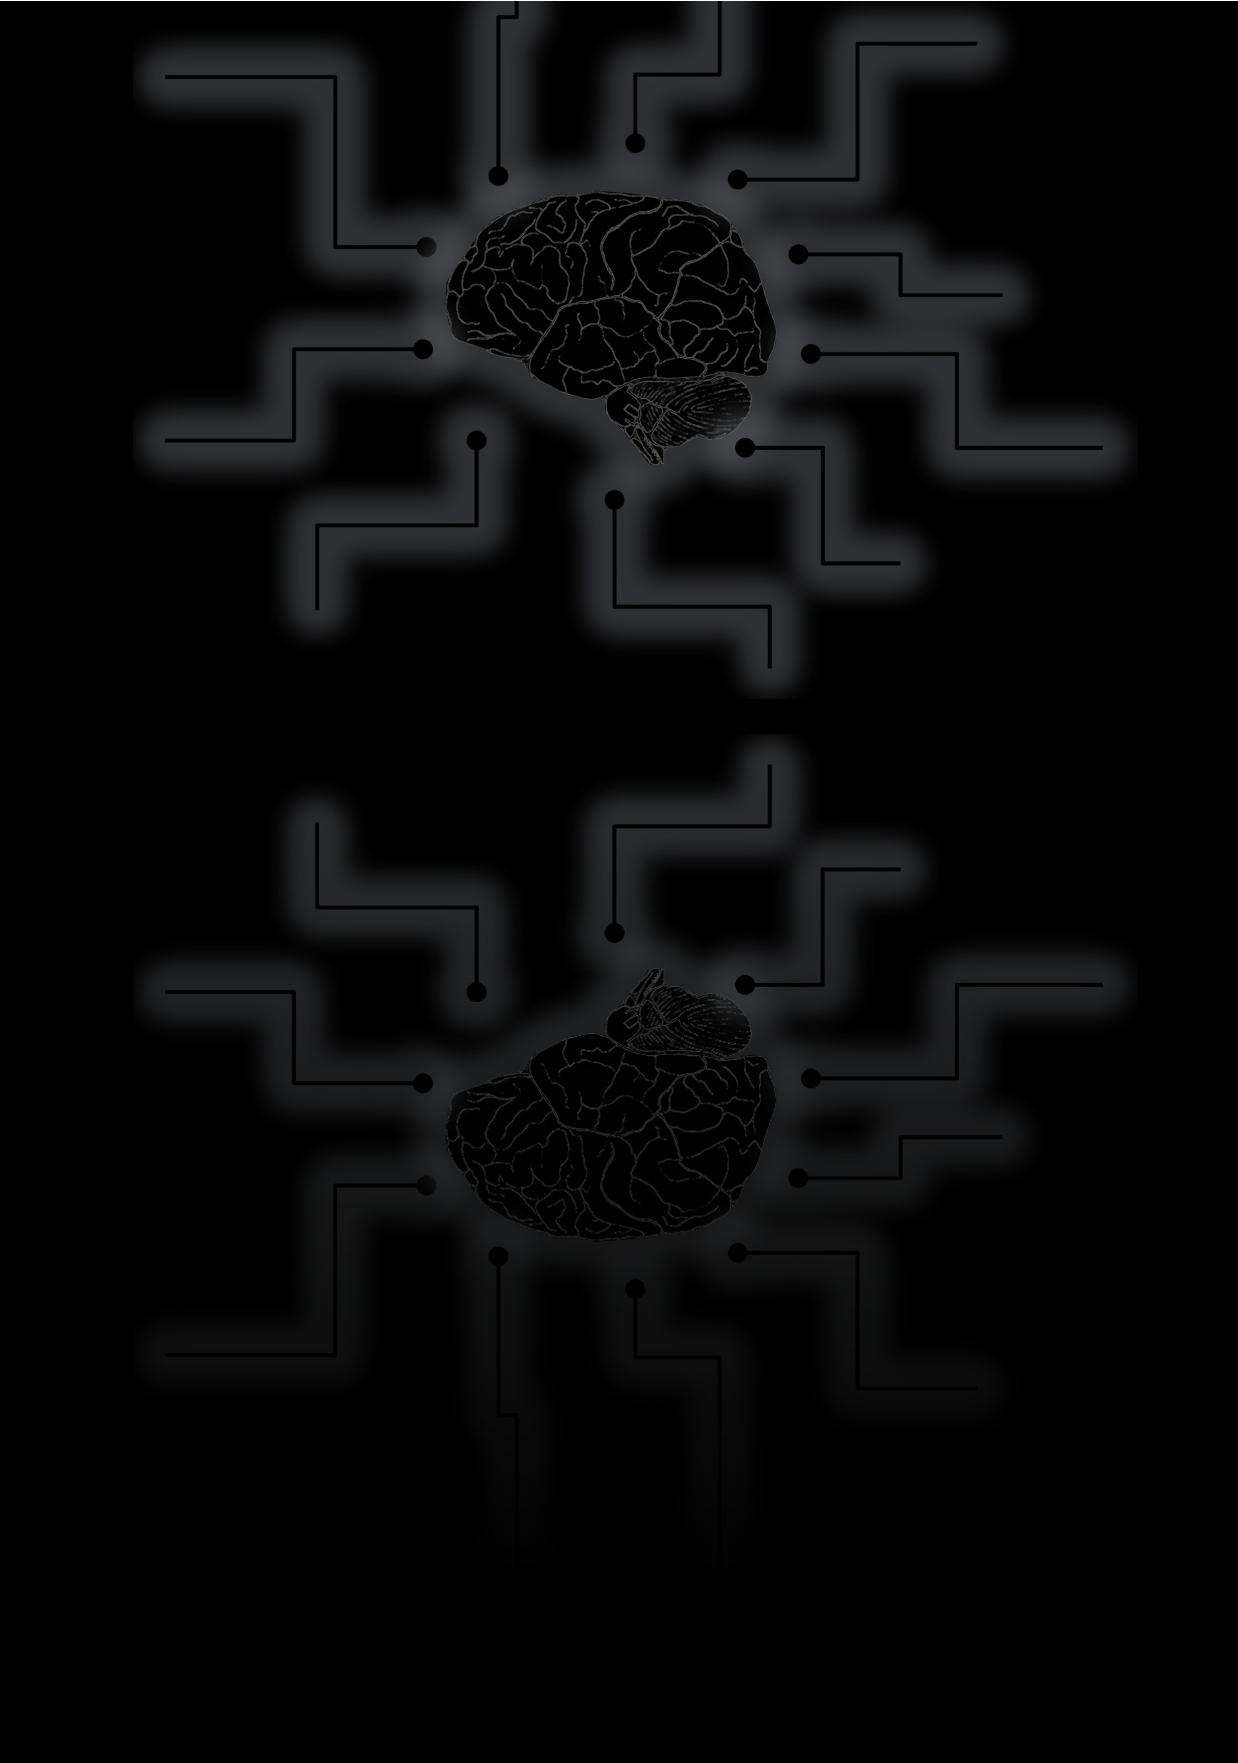
\includegraphics[width=\paperwidth]{Cover.pdf}};
\draw (current page.center) node [fill=black,fill opacity=0.0,text opacity=1,inner sep=1cm,yshift=2cm]{\Huge\centering\bfseries\sffamily\parbox[c][][t]{\paperwidth}{\centering\color{white} Research in Practice:\\ {\Large A Methods Handbook for Research\\ in the Psychological Sciences\\}% Book title
% Subtitle
\vspace{.5cm}
{\small Paul D. Kieffaber, Ph.D. \\ {\color{gray!40} College of} {\color[rgb]{.06,.339,.25} William} {\color{gray!40} \&} {\color[rgb]{.722,.589,.355} Mary}}}}; % Author name
\end{tikzpicture}
\vfill
\endgroup

%----------------------------------------------------------------------------------------
%	COPYRIGHT PAGE
%----------------------------------------------------------------------------------------

\newpage
~\vfill
\thispagestyle{empty}

\noindent Copyright \copyright  2021 Paul D. Kieffaber\\ % Copyright notice

\noindent \textsc{Published by Publisher} \\ % Publisher

\noindent \textsc{https://wmpeople.wm.edu/site/page/pdkieffaber/home}\\ % URL

\noindent Licensed under the Creative Commons Attribution-NonCommercial 3.0 Unported License (the ``License''). You may not use this file except in compliance with the License. You may obtain a copy of the License at \url{http://creativecommons.org/licenses/by-nc/3.0}. Unless required by applicable law or agreed to in writing, software distributed under the License is distributed on an \textsc{``as is'' basis, without warranties or conditions of any kind}, either express or implied. See the License for the specific language governing permissions and limitations under the License.\\ % License information, replace this with your own license (if any)

\noindent \textit{First printing, March 2019} % Printing/edition date

%----------------------------------------------------------------------------------------
%	Author Credits
%----------------------------------------------------------------------------------------
\newpage
\thispagestyle{empty}
\begin{center}Author Credits\end{center}
\begin{itemize}
    \item Sensation \& Perception - Parts of the chapter were adapted by material originally developed with support from the William \& Flora Hewlett Foundation, Bill \& Melinda Gates Foundation, Michelson 20MM Foundation, Maxfield Foundation, Open Society Foundations, and Rice University. Powered by OpenStax CNX.
    \item Hello
\end{itemize}



%----------------------------------------------------------------------------------------
%	TABLE OF CONTENTS
%----------------------------------------------------------------------------------------

%\usechapterimagefalse % If you don't want to include a chapter image, use this to toggle images off - it can be enabled later with \usechapterimagetrue

\chapterimage{ChapterCover.pdf} % Table of contents heading image

\pagestyle{empty} % Disable headers and footers for the following pages
\dominitoc% Initialization of minitoc
\tableofcontents % Print the table of contents itself

\cleardoublepage % Forces the first chapter to start on an odd page so it's on the right side of the book

\pagestyle{fancy} % Enable headers and footers again

%----------------------------------------------------------------------------------------
%	SECTIONS/CHAPTERS
%----------------------------------------------------------------------------------------
%\part{Essential Computing Competencies}

%----------------------------------------------------------------------------------------
%	Introduction to PsyToolkit CHAPTER 
%----------------------------------------------------------------------------------------
\chapterimage{ChapterCover.pdf} % Chapter heading image
\chapter{Methods for Data Collection}

\epigraph{\textit{I do not fear computers. I fear lack of them.}}{\rightline{{\rm --- \href{https://en.wikipedia.org/wiki/Isaac_Asimov}{Isaac Asimov}}}}

\minitoc
\newpage
\section{Software for Generating Experiments}
The advent of desktop-computers forever changed the landscape of research in nearly all scientific fields.  For psychological science, desktop computers have made possible new ways of probing the cognitive, emotional, and social functions of the brain. In addition to software that facilitates data management and analysis, computers can be used for flexible and precise control over many aspects (e.g.., stimuli and responses) of experimental procedures. It is their central role in the scientific process, from experimental design, to data collection, to data analysis, to typesetting a formal report of the results that makes a broad range of computing skills so critical to success in the psychological sciences. Of course, each aspect of research requires its own set of computing competencies. Here, emphasis will be placed on the design of experiments and collection of data. 

\subsection{Choosing the Right Software}
\subsubsection{Commercial Vs. Open Source}
As with any task you wish to complete on a computer, there are several commercial and \gls{open source software} options available. In the case of generating psychological experiments, all of the available options provide methods for displaying text, images, sound, and/or video as well as methods for recording responses using the keyboard, mouse, or other peripheral device like a specialized button box.  The authors/distributors of these software packages also claim to provide accurate control of experiment timing, usually to within a millisecond. 

Both the open source and the commercial options have their strong advocates. One argument is that the open-source method of developing software is far superior to commercial methods. Users of open source software have access to the source code, meaning they can enhance the program’s performance, add features, and fix errors. In fast-paced scientific fields, this can mean that open source software will likely be the first to implement the latest and greatest methods. In the event of the establishment of novel methods, those who develop commercial software (a.k.a. ``closed source software") must employ their programming team to implement the method within their software and run exhaustive testing in order to be able to provide assurance of accuracy/reliability to their customers before releasing a software update. 

The most staunch proponents of commercial software often argue that this assurance of accuracy and reliability is precisely what makes it preferable to open source software.  Another advantage of commercial software is the product support that is offered along with purchase of the software.  If you download software like PsychoPy and receive an error when you attempt to install it, or are unable get it working properly after installation, your only option is to post your question to one of the online discussion boards dedicated to PsychoPy, and hope for a response.  On the other hand, if you purchase a license to use E-prime\copyright and have trouble installing the software and/or running an experiment, you can call the company and speak to an employee who's job it is to help you solve your specific problem. Ultimately, there are costs and benefits of both commercial and open source software and selection of a specific program should, most importantly, be based on how well that software will facilitate your research agenda.

\subsubsection{Flexibility Vs. Ease of Use}
Experiment control software also varies considerably on dimensions of flexibility and ease of use. Unfortunately, these two important dimensions tend to be inversely related to one another (see Figure \ref{fig:ExpCtrlApps} in almost any programming context. The reason for this inverse relationship is computers only do \emph{exactly} what you tell them to do.  When it comes to designing an experiment, instructing the computer about the many related details such as what image should appear on the monitor, where it should appear, how long it should remain on the monitor, whether or not to record a response from participants in your experiment all can be quite complicated. 

\begin{wrapfigure}{R}{0.5\textwidth}
\begin{tcolorbox}[every float=\centering, drop shadow, title=Trade off between Flexibility and Ease of Use ,colback=WMgold,colframe=WMgreen,
  colbacktitle=WMgreen,]
  \begin{tikzpicture}[%
    filled/.style={circle,fill=WMgreen,text=white,font=\large},
    label distance=4pt]
\coordinate (O) at (0,0);
\draw (-3,-3) -- (3,-3);
\draw (-3,-3) -- (-3,3);
\node [above right, align=center,filled] at (-2,0) {More\\Programming};
\node [above right, align=center,filled] at (.5,-2.2) {More\\Point \& Click};
\node [below, align=center] at (0,-3) {Ease of Use};
\node [left, align=center, rotate=90] at (-3.3,1) {Flexibility};
  \end{tikzpicture}
  \captionof{figure}{Illustration of the trade-off between flexibility and ease of use in experiment control software}
  \label{fig:ExpCtrlApps}
 \end{tcolorbox}
 \end{wrapfigure}
 
Software that is easy to use tends be more ``point \& click", meaning that the software's author(s) have, in order to simplify the process of creating an experiment, reduced the number of instructions you are required to give to the computer by implementing a number of assumptions about how the experiment should run.  Although these assumptions effectively relieve everyday users of the burden of having to understand much of the underlying programming language, this ease of use often comes at the cost of flexibility. Finding a good balance of flexibility and ease of use is important so that novel and/or dynamic research needs can quickly be addressed but implementation of those needs does not require complete mastery of a programming language. While a complete review of the available software is beyond the scope of this chapter, software reviews do occasionally appear in the literature \citep[e.g.,~][]{stahl2006software}.

Most commercial software is available through stand-alone packages, meaning that once the software has been purchased, there are no other dependencies or packages required other than those that are already installed on your computer. Some examples of commercial software are \weblinkT{https://pstnet.com/}{E-prime\copyright}, \weblinkT{https://cedrus.com/superlab/index.htm}{SuperLab}, \weblinkT{https://www.neurobs.com/}{Presentation}, and \weblinkT{https://www.empirisoft.com/DirectRT.aspx}{DirectRT}, just to name a few. It can be quite difficult to draw direct comparisons between these different options because each one has a unique set of strengths and weaknesses and are typically designed to meet the needs of users in specific research contexts. For example, two historically popular choices are E-Prime and SuperLab, each of which offers an easy to use point \& click style interface with which simple experiments can be generated in just a few minutes. Another popular commercial option is Presentation.  Although Presentation does not have the same kind of graphic user interface (GUI) as E-prime\copyright or Presentation, the language includes a powerful set of commands for designating experimental components (e.g., images, sounds, responses etc.) and their timing (e.g., onset, offset, duration, etc.).

 A popular open-source option for the generation of experiments is \weblinkT{http://psychtoolbox.org/HomePage}{Psychtoolbox}. With years of development and a broad base of users, Psychtoolbox boasts a wide variety of powerful, well-developed routines for experimental control. However, Psychtoolbox is written in the Matlab programming language, meaning that using it requires that you have a licensed installation of Matlab. Thus, while Psychtoolbox is freely available, there is an indirect, prerequisite cost of obtaining Matlab\footnote{Note that the latest version of the Psychtoolobx is also compatible with GNU Octave, a free alternative to Matlab}. Like Presentation, Psychtoolbox lacks a GUI so even simple experiments require at least some experience with the Matlab programming language, making it difficult for new users without much programming experience.
 
Another open source option is \weblinkT{https://www.psychopy.org/}{PsychoPy}. Written in the Python programming language, itself a free alternative to programs like Matlab, PsychoPy offers an attractive balance of flexibility and ease-of-use.  PsychoPy has the full flexibility of any general purpose programming language, but also includes a user-friendly GUI with point \& click features that allow simple experiments to be generated with little to no knowledge of the Python programming language.

\subsubsection{Online Data Collection}
The ability to collect data online using experiment control software is a feature that has recently become especially popular.  In fact, most commercial \emph{and} open source software offers some kind of online option for data collection, but it is important to understand at least two of the central issues related to collecting data online, including  (1) the type of data being collected and (2) how will the data be stored.

The type of data being collected in an online experiment is an important consideration because some measures of behavior and/or parameters of a stimulus display require a degree of temporal precision that may be difficult to achieve in practice.  For example, an accurate measure of reaction time requires (1) precise measurement of the time at which a stimulus is presented to the participant (i.e., the stimulus to which participant is reacting) and (2) an accurate measure of the time at which a key or button was pressed.  These may seem trivial, but while computers only do exactly what they are told, they don't always do it exactly when they are told. 

Remember that modern computers are serial processors, managing many different tasks such as checking your email inbox, running virus protection software, monitoring internet traffic, etc., all while also running your experiment. Each of these tasks uses some of a limited set of resources on the computer. When the program you are using instructs the computer to display an image or play a sound, the expectation is that it will happen immediately, but this is almost never the case. Instead, the time between the instruction to present a stimulus and the appearance of that stimulus to the participant depends on a variety of factors like the amount of available resources at that moment, the priority assigned to your experimental task by the computer's CPU relative to other ongoing computer functions, characteristics of the computer's video and/or audio cards, and other computer hardware and software settings.  There is also uncertainty in the measurement of key/button press responses.  Computers only "check" the status (i.e., up/down) of keys and buttons at designated intervals; typically 125 times per second or every 8 milliseconds.  This \gls{polling rate} can vary from computer to computer, from device to device, and can also be influenced by the resources currently available to the computer's CPU.  In short, most of this uncertainty about the precision of stimulus and response timing contributes to random \gls{measurement error} in the assessment of reaction times, however, systematic measurement errors can also occur when hardware or software introduces consistent differences between the measured and true reaction times.
\myfigure{Error in online RT Measurement}{PsyToolkit/Figures/MeasurementError.png}{Illustration of Measurement Error in RT that can occur with online data collection.}{fig:measurmenterror}{\linewidth}{.87\linewidth}{.1\linewidth}

\begin{wrapfigure}{R}{0.45\textwidth}
\begin{tcolorbox}[width=.95\textwidth,colback=yellow!5!white,colframe=yellow!50!black,
  colbacktitle=yellow!75!black,title=Food For Thought,grow to right by=1cm]
  \emph{How might online data collection involving the collection of reaction times potentially introduce a confounding variable to your research?}
  \tcblower
  When each participant uses their own computers, each with different components and specifications that contribute to error in the accuracy of RT measures, there is an increase in both random and systematic measurement error between subjects. This can be particularly problematic for studies involving between-groups designs because there is the possibility that systematic differences in reaction time may exist because of systematic differences between the quality of the computers used by the two groups. 
\end{tcolorbox}
\end{wrapfigure}
 All of the concerns just mentioned are compounded with the recording of reaction times over the internet. This is because both random and systematic measurement error can be expected to be relatively consistent from person to person when all of the participants complete your experimental task on a computer in your laboratory.  When the participants each use their own computer, the degree to which random and/or systematic measurement errors influence the recorded reaction times will, in addition to being unknown, fluctuate from person to person. This potential increase in error variability between subjects can mean that more participants will be required for online research involving reaction times and/or precise control over stimulus timing.

It is also important to consider how the data will be stored in an online experiment.  Here data storage refers to the how and where data will be stored as the participant is responding to the items on your questionnaire or stimuli in your experiment rather than how/where the compiled data will be stored after the experiment has ended and data analysis begins.  In order to understand this distinction, it is important to have a basic understanding about what happens when you send a participant the link to your questionnaire or experiment.

There are many facets of hosting a web page that collects data from participants that we don't really need to get into here, but the important thing is that when your participants visit a website, a series of things are happening:
\begin{enumerate}
    \item You set up your web page using your favorite program and send the link to your participants.
    \item Participants use their web browser to enter the link, which sends a request to the website's server for a page, a document, or a file for running an application. The \gls{URL} or address you put into the bar at the top of the browser window is the main portion of that request.
    \item The web server receives the request and pulls together whatever it needs to deliver back to the participant what they requested. This might just be an existing file, or it might be a piece of a web application, or it might be an assembled document from a content management system.
    \item The participant's browser application shows them the content and communicates back to the server about the participant's responses.
\end{enumerate}
So, in order to host a website for data collection, you need a computer running server software capable of managing requests from many simultaneous participants and that is \emph{always} connected to the internet so it can respond to requests and store data at any time.  Of course, this isn't the kind of thing that your standard desktop computer is capable of doing, so you will need a website server, which can be expensive and difficult to maintain.  Thus, the most common approach to online data collection is to subscribe to a \gls{web hosting service}, which provides all of the services above for a fee.

Although online surveys for data collection have been readily available and used for decades (e.g., Qualtrics\copyright), options for developing online experiments that involve presenting participants with controlled stimuli and recording responses like reaction time and accuracy have only recently become available. Some commercial software applications (e.g., E-prime\copyright) are beginning to offer web hosting services as part of their software license. Developers of the open source software PsychoPy have also developed an online platform called \weblinkT{https://www.psychopy.org/online/usingPavlovia.html}{Pavlovia} that is capable of hosting online experiments created using PsychoPy. Using Pavlovia, only requires the purchase of ``credits" that are redeemed as participants connect to and complete your experiment(s).  Yet another, completely free alternative is \weblinkT{https://www.psytoolkit.org/}{PsyToolkit} \citep{stoet2010psytoolkit,stoet2017psytoolkit}. PsyToolkit is a free-to-use toolkit for demonstrating, programming, and running cognitive-psychological experiments and surveys, including personality tests. PsyToolkit is frequently used for academic studies, for student projects, and for teaching cognitive and personality psychology. An advantage of PsyToolkit is that it works in most web browsers and so is completely \gls{platform independent}.  Another advantage is that surveys and experiments can be created \emph{and} hosted on their website for free.  However, remember the trade off between flexibility and ease of use described earlier.  A flexible platform for data collection, PsyToolkit requires learning its scripting language, which can be challenging for those with little or no prior programming experience.

Whichever software or platform you choose for your specific research needs, time and effort will be required to learn how to use it when designing your data collection protocol.  Tutorials for several open source software packages are provided in the following sections, however, before tackling the task of learning to program an experiment, let's consider the research context for these tutorials.

\section{Research in Practice}
Today, even most children in the 1st grade would likely answer correctly when asked whether the brain is the source of human thought (the answer is yes!). However, it is important to remember that it was only as recent as the latter part of the nineteenth century that this became consensus in the scientific community. Medical observations like that of Phineas Gage (1823-1860), an American railroad construction worker who survived an explosion that drove a large iron rod completely through his head, fueled that understanding and helped to shape modern thinking about brain-behavior relationships. Although the accident destroyed much of his left frontal lobe, the most profound changes following Mr. Gage's accident were with regard to his personality and behavior. In other words, the damage Mr. Gage suffered to his brain seemed to have a direct effect on complex thought. This was important because there was considerable debate at the time as to whether this kind of “thought” was something material or non-material (e.g., ``mental", or ``spiritual") and observations of Mr. Gage’s experience with brain damage supported the notion that complex thought, like other aspects of behavior, had a material basis in the central nervous system.

Interestingly, at about this same time in the middle part of the 1860’s, Franciscus Cornelis Donders, a Dutch physiologist, conceived of a way to measure “thinking” in the laboratory. His novel idea was that if thought is material, then it may be measurable in terms of the time taken to generate thoughts. But how does one measure the time taken to think (especially in the 1860’s!)? To show that thinking takes time, Donders used an elegantly simple subtractive logic. He began by measuring the time required to execute an action (e.g., press a button) following perception of a stimulus (e.g., a light; sometimes called the ``simple" reaction time), reasoning that this response time reflected the sum of the times taken to detect the stimulus and execute the response. Donders then used this simple reaction time as a baseline for comparison with tasks that involved more ``thinking". Provided that the stimuli and responses are the same as those used to measure simple reaction time, any additional time taken to complete a task involving more ``thinking" must be attributable to the time it takes to produce that ``thinking". 

Fundamental to Donder's logic was the idea that mental processes can be described as stage-like ``thought" units. Until Donder's work, many assumed that mental operations likely occurred in parallel and instantaneously. One of Donder's primary goals was to elucidate the timing of mental operations using his simple subtraction technique. In his now famous 1868 research, Donders used three different tasks: (1) The first task was a simple reaction time task wherein participants responded as quickly as possible upon detecting a stimulus. (2) The second task was a so-called Go/No-Go discrimination reaction time task in which participants were instructed to press a button only when a target (i.e., Go) shape appeared, but to withhold their response if a different, non-target (i.e., No-Go) shape appeared. (3) Finally, the third task was a choice reaction time task in which there was more than one target and participants were instructed to make different responses to each target (see Figure \ref{fig:donders}).
\begin{center}
\myfigure{Donders Reaction Time Tasks}{PsyToolkit/Figures/Donders.png}{Illustration of the three Donders reaction time tasks and the subtractive logic used to infer the timing of mental events.}{fig:donders}{.8\linewidth}{.82\linewidth}{.15\linewidth}
\end{center}

Donder’s hypothesized that four kinds of cognitive processes were involved in these tasks: (1) The simple reaction time task would require just two of these processes, perception (detecting the light) and action (pressing the button). (2) The Go/No-Go discrimination task would require the same perception and action processes as in the simple reaction time task, plus a discrimination process in which the participant must determine whether the stimulus was a target (i.e., Go) or non-target (i.e., No-Go). (3) Finally, the choice reaction time task was reasoned to require all of the same processes required for the simple and discrimination reaction time tasks, plus a response selection process in which the participant must decide which response to execute. 

As you might expect, the simple reaction time task is typically associated with the fastest reaction times, followed by the discrimination (e.g., Go/NoGo) task, followed by the choice reaction time task. Donders then proposed that the time required for each mental operation (i.e., thought) could be calculated by simple subtraction. For example, the time it takes to identify a stimulus could be calculated by subtracting the simple reaction time (i.e., perception + action) from the RT in the Go/No-Go task (i.e., perception + identify stimulus + action). While this technique has not been used without criticism, this basic procedure for isolating component cognitive processes remains the basis of the logic behind much of the research in the Psychological Sciences today.

Although Donders did not have access to computers (In fact, he had to develop new technology to make precise measurements of reaction times), this kind of experimental procedure can be easily replicated today using software like PsyToolkit, PsychoPy, and/or PsychToolbox.

\section{PsyToolkit}\index{PsyToolkit}
Developed in the mid 2000s, PsyToolkit is a free platform for programming and running psychological experiments that runs within web browsers using Javascript and HTML5 technology to achieve performance that is comparable to commercial software like ePrime \citep{kim2019testing}.  Although used primarily as an online platform for data collection, it can also be used offline as an in-laboratory software.

Unlike other popular programs, PsyToolkit is entirely script-based programming and there is no point-and-click graphical user interface for setting up an experiment. As was mentioned earlier in this chapter, this has advantages and disadvantages. The disadvantage is that it can take more time to learn. The advantage is that it can be much more flexible and, once mastered, faster to program simple experiments than in other similar software.  This tutorial will introduce you to the basics of creating surveys and experiments using PsyToolkit. Further details and answers to FAQs can be found on their website at \weblinkT{https://www.psytoolkit.org/}{https://www.psytoolkit.org/}.

\subsection{Getting Started with PsyToolkit}
\begin{enumerate}
    \item Go to: \weblinkT{https://www.psytoolkit.org/}{https://www.psytoolkit.org/}
    \item Click \textbf{Web based / login} and then click the link to register for a free web-based account.
    \item A password will be sent to you via email
    \item Use your email and password to sign in to begin creating your first experiment! (see Figure \ref{fig:psytoolkitlogon}
\end{enumerate}

\begin{center}
\myfigure{PsyToolkit Login Page}{PsyToolkit/Figures/psytoolkitlogon.png}{The PsyToolkit login page. Use your email address and the password sent to you when you created your free account.}{fig:psytoolkitlogon}{.8\linewidth}{.8\linewidth}{.17\linewidth}
\end{center}

\subsection{Create Your First Survey}
Once you have logged into your PsyToolkit account, you will be taken to your home page where you can see announcements from the developers, tips about using PsyToolkit, and links (in the frame on the left) to general settings and tools for creating and editing experiments and surveys (see Figure \ref{fig:psytoolkithome}).  In PsyToolkit, experiments are deployed from within surveys, so we will start this tutorial by creating a survey and later show how to add an experiment.

\myfigure{PsyToolkit Home Page}{PsyToolkit/Figures/psytoolkithome.png}{The PsyToolkit user's home page with access to personal and public libraries of surveys and experiments.}{fig:psytoolkithome}{\linewidth}{.8\linewidth}{.17\linewidth}
You can start creating your first survey right away by following these two simple steps:
\begin{enumerate}
    \item Click ``Create new survey"
    \item Enter a name for your survey and click ``Create completely new online survey"
\end{enumerate}
Following these two steps will open the Survey Editor where you can create your survey.  By default, new surveys include several sample items (see Figure \ref{fig:psytoolkitsurvey}).

\myfigure{PsyToolkit Home Page}{PsyToolkit/Figures/PsytoolkitSurveyEditor.png}{Creating an Online Survey.}{fig:psytoolkitsurvey}{\linewidth}{.8\linewidth}{.17\linewidth}

Each item of a survey can be created with just a few lines of text, however, there are strict rules governing the syntax of that text.  Each item is defined by a set of ``label", ``type", and ``question" parameters and, in some cases, a list of options defining the response(s) available to the participant. Each of the parameters that define the survey item is designated by an \texttt{l} (label), a \texttt{t} (type), or \texttt{q} (question), followed bye a colon and then the parameter definition (see \ref{code:psytoolkitquestion}).  Some item types also include an ``options" parameter.  Several examples of survey items are illustrated below. For complete details about the structure of surveys and items, refer to the \weblinkT{https://www.psytoolkit.org/doc2.4.0/online-survey-syntax.html}{Online Surveys} tutorial page.  

\begin{tcolorbox}[every float=\centering, drop shadow, title=PsyToolkit - Checkbox Example]
    \begin{minipage}[t]{0.9\linewidth}
    \vspace*{0pt}
    \begin{verbatim}
l: examplequestion2
t: check
q: Select all of the following drinks did you had today?
- Water
- Orange juice
- Tea
- Coffee
\end{verbatim}
    \end{minipage}\hfill%
    \tcblower
    \begin{center}
    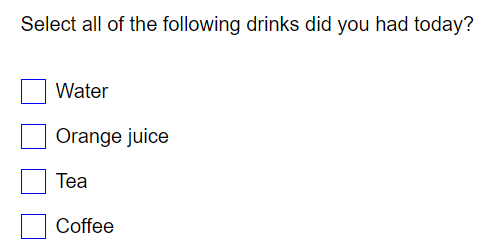
\includegraphics[width=.5\linewidth]{PsyToolkit/Figures/SurveyCheckbox.PNG}
        \label{fig:checkboxexample}
    \end{center}
    \begin{codeblock}{PsyToolkit code (top) and preview (bottom) for creating a simple question with checkbox options.}\label{code:psytoolkitquestion}\end{codeblock}
\end{tcolorbox}

Of course, when you are just starting out with PsyToolkit, the process of creating an entire survey with many different question types can seem a bit daunting.  Fortunately, PsyToolkit also offers an ``Easy" mode that can be especially helpful for beginners.  To enter easy mode, simply click the button labeled ``easy mode" just above the survey editor (see Figure \ref{fig:psytoolkiteasymode}). 

\mywrapfigure{PsyToolkit Easy Mode}{.5\linewidth}{PsyToolkit/Figures/PsytoolkitEasyMode.PNG}{Adding survey items is as simple as a few clicks using ``Easy Mode".}{fig:psytoolkiteasymode}
When in easy mode, the items in your survey are listed in a convenient table that includes links to enable direct editing of each item.  New items can be added by clicking the \button{+} button.  When you add a new item, you will first be presented with a list of available item types.  The decisions you make about the types of items you include will be based on the kind of data you wish to collect and the parameters you want to impose on the participant's responses.  For example, most surveys will include an item requesting the participant to indicate their gender.  One possibility would be to use a text line where the participant can enter whatever response they like using the keyboard. In this case, it will be up to you as the researcher to comb through the responses and group similar responses like ``male", ``Male", ``M", ``boy", or maybe even ``mail".  This could be a tedious and error-prone process, so a more appropriate choice when requesting the participant's gender might be to use the radio button type item with options for ``Male" and "Female", which would simplify data entry for the participant \emph{and} data analysis for the researcher.  In short, you should carefully consider how you select items for your survey.  You can add as many items to your survey as you like.

Of course, items are the most important part of your survey as they determine the kinds of information/data that are collected.  However, whenever collecting data from human participants, it is important to provide them with enough information about the study that they can make an informed decision about whether or not they would like to participate \emph{before} you start collecting data.  This kind of information that is required for \gls{informed consent} is also designated in the survey design page using the text fields available in the ``Survey intro screen and special options" section of the PsyToolkit survey generation page.  

If you are still in easy mode, you will first need to return to the regular mode by clicking the \button{regular overview} button (see Figure \ref{fig:psytoolkiteasymode}). Next, scroll down to the ``Survey intro screen and special options" section.  There you will find options governing the look and feel of your survey, an ``About this survey" section where you can enter information to be provided to the participant \emph{before} they begin the survey, an expandable ``Read more" section for additional information, and a ``Contact information" section where you can provide the participant with contact information for the \gls{principal investigator} (PI). Once you have entered all of this information (\emph{don't forget to click the \button{Click to save} button at the bottom!}), you are ready to compile and test your survey.

\subsubsection{Test Your Survey}
Before you deploy your survey you will, of course, want to test it out.  This requires that you first \gls{Compile} your survey for execution. If you are still in easy mode, you will first need to return to the regular mode by clicking the ``regular overview" button (see Figure \ref{fig:psytoolkiteasymode}) and take the following steps:

\begin{enumerate}
    \item Scroll down to the ``Compile/test survey" section and click the \button{compile} button (see Figure \ref{fig:psytoolkitcompilesurvey}).
\myfigure{Compile/test your survey}{PsyToolkit/Figures/PsytoolkitCompileSurvey.PNG}{Use the ``Compile" button to compile and test your survey.  You will get a message letting you know if there were errors or if it compiled correctly.}{fig:psytoolkitcompilesurvey}{\linewidth}{.76\linewidth}{.23\linewidth}
Note that if your survey does not compile correctly PsyToolkit is designed to give detailed feedback of how to fix errors. PsyToolkit will tell you which line of your script file the problem occurs in.  If you are having trouble getting your survey (or experiment) to compile, you may want to check the Problem solving \& Tips page at \weblink{https://www.psytoolkit.org/software/problemsolving.html}.

\item Once your survey has compiled successfully, scroll down to the ``Online/Offline survey status" section and select the option, ``Survey is online. For when you are still designing it." and then click the \button{Change survey status} button.
\myfigure{Compile/test your survey}{PsyToolkit/Figures/PsyToolkitTestStatus.PNG}{Use the ``Compile" button to compile and test your survey.  You will get a message letting you know if there were errors or if it compiled correctly.}{fig:psytoolkitteststatus}{\linewidth}{.76\linewidth}{.23\linewidth}

\item When the status has been changed, you will be provided with a \gls{URL} that can be copied into the address bar of your browser which will take you to the online survey (see Figure \ref{fig:psytoolkitteststatus}).
\end{enumerate}

When you follow the link to your survey, you will first see all of the information provided in the ``About this survey" section.  Once the button is clicked to start the survey, each of the items is presented one-by-one until all of the items have been answered (see Figure 

\subsubsection{Check the Survey Data}
All responses are automatically saved any time the survey is completed.  In order to view and/or download the data, simply scroll to the bottom of the page used to edit your survey in PsyToolkit and find the ``Prepare and download participant data" section.  Click the \button{Prepare datafiles for download} button.  Soon thereafter (after a couple of refreshes), a \button{download data in zip file} button will appear.  Click that button to download your data (see Figure \ref{fig:psytoolkitdownload}).

\mywrapfigure{PsyToolkit Data Download}{.5\linewidth}{PsyToolkit/Figures/PsyToolkitsurveydownload.PNG}{PsyToolkit Data Download}{fig:psytoolkitdownload}

The data files will be compressed into a single .zip file.  When you find the downloaded file, uncompress (i.e., unzip) it to your favorite location on your computer.  The unzipped folder will be called ``data" by default.  Inside, you will find a number of files, including a copy of the original survey script file in ``survey.txt", individual text files containing raw data from each of the participants separately, the participant's \gls{aggregate data} in ``data.csv" and ``data.xlsx" (two formats are provided for convenience), and aggregate data about the times/dates when the surveys were completed in ``data\_times.csv" and ``data\_times.xlsx". 

It may take some time to understand how your data are organized.  Although each row of the tabular output is dedicated to one of the participants, each of the item types has a slightly different data storage format.  For example, the ``radio" items only allow for one response to be selected, so the result is stored in a single column (see Figure \ref{fig:psytoolkitdataformat}).  The ``check" item types allow users to select multiple items, so each of the available responses is listed as a column and a \texttt{0} or a \texttt{1} is used to indicate the absence/presence of a check-mark for that item (see Figure \ref{fig:psytoolkitdataformat}).

\myfigure{Aggregate Survey Data}{PsyToolkit/Figures/PsyToolkitDataFormat.PNG}{Aggregate Survey Data.}{fig:psytoolkitdataformat}{\linewidth}{.82\linewidth}{.17\linewidth}

\subsubsection{Deploy Your Survey}
It is important that you inspect and understand the aggregated output from PsyToolkit \emph{before} you deploy your survey to participants. Imagine that, only after putting all the time and effort into designing a survey, coding it in PsyToolkit, and collecting data from participants, you find out that a critical piece of information is missing from your survey or that the data you collected aren't appropriate for the analysis you had in mind.  Although it can take some time, thorough testing can mean the difference between a successful and a failed research project. That said, once you have thoroughly tested your survey, it is a simple matter to deploy it for real data collection using the following steps.

\begin{enumerate}
    \item First, it is usually a good idea to clear the data recorded while testing. Scroll to the bottom of your survey's page in PsyToolkit and click the \button{delete participant data files} button.
    \item Next, scroll up to the ``Online/Offline survey status" section and select the ``Survey is online. For when real data collection is going on" option and then click the \button{change survey status} button.
\end{enumerate} 

%\begin{wrapfigure}{R}{0.35\textwidth}
\begin{wrapfigure}[16]{R}[0pt]{.35\textwidth}
\begin{tcolorbox}[width=\textwidth,colback=yellow!5!white,colframe=yellow!50!black,
  colbacktitle=yellow!75!black,title=Food For Thought,grow to right by=1cm]
  \emph{Even creating a simple survey requires creativity and critical thinking!}
  \tcblower
  When a researcher creates an instrument for their research like a survey or experiment, there are many different decisions that must be made along the way.  For example, if you decide to ask your participants to indicate their gender, do you use male/female radio buttons, a text box that will permit a free response, or a drop-down menu.  These decisions will impact the experience of participants as well as the format of the recorded data, which may later impact the researcher's approach to data analysis.  In short, survey and experiment design are important skills for any psychological scientist.
\end{tcolorbox}
\end{wrapfigure}
You will again be provided with a link to your active survey.  This link can be shared with anyone you would like to complete your survey (or even shared publicly).  The only difference now is that your survey cannot be modified until you again change its status in PsyToolkit.

\subsection{Create Your First Experiment}
In the previous section, we covered how to create and deploy a simple survey using PsyToolkit. In the following sections we will see how to create and deploy experiments. While both survey and experiment methods are important in data collection and both can be used to test hypotheses, experimental research involves the manipulation of an independent variable and measuring its effect on a dependent variable.  In the context of research in the psychological sciences, the dependent variables are commonly measures like reaction time, accuracy, and number of items remembered while the independent variables are typically physical properties of the experimental stimuli like color, shape, emotional valence, and duration of exposure. In the following tutorial we will cover the steps necessary to create a simple reaction time task using PsyToolkit.  More advanced examples and detailed information can be found in the online documentation at \weblinkT{https://www.psytoolkit.org/doc3.2.0/}{https://www.psytoolkit.org/doc3.2.0/}.

Before you get started programming your task, it is always a good idea to lay out a specific plan. In this example, the aim is to re-create the simple reaction time task from the Donders experiments described earlier.  Thus, the experiment will minimally consist of the following: \begin{itemize} \item Presentation of  a fixation point (used to direct the attention of the participant) \item Presentation of a target stimulus \item Detecting and recording response times \end{itemize}  Identifying all of the major components of a task can be made easier by developing a \gls{task schematic} (see Figure \ref{fig:schematic}).  The task schematic will often illustrate the experimental stimuli, highlight the major parameters of an experimental task such as the time between stimuli, called the \gls{inter-stimulus interval} (ISI), and show how responses were collected from participants.

Working from the task schematic in Figure \ref{fig:schematic}, we can see that programming this experiment will require  at least two visual stimuli that will be presented to the participant, the fixation cross and the target stimulus (a diamond shape in this case) and the collection of a response from the keyboard.  We will also need to define an ISI and and an \gls{inter-trial interval} (ITI; not shown in the schematic) which will determine how much time should elapse between the response to one stimulus and the appearance of the fixation cross indicating the impending appearance of the next stimulus.

\myfigure{Example of a Task Schematic}{PsyToolkit/Figures/schematic.PNG}{The task schematic makes explicit the parameters of an experiment and can serve as a planning tool during programming \emph{and} as a visual aid for readers at the time of publication.}{fig:schematic}{\linewidth}{.5\linewidth}{.45\linewidth}
Creating a task schematic before you begin programming an experiment can be a useful in that is provides a convenient visual reference when determining how to program your experiment and it can also serve as a visual aid for readers when the experiment is completed and you are presenting the results of your experiment. For now, the task schematic can be used to determine the stimuli that need to be created. 

\subsubsection{Creating the Stimuli}
After having planned out your experiment but before beginning the work of programming that experiment in PsyToolkit, it is prudent to create the experimental stimuli (i.e., images and sounds) that will be presented to participants.  For present purposes, we will focus on the two images that will be presented to participants in the simple reaction time task, namely the fixation cross and the diamond shape.

PsyToolkit works best with a particular type if image file called a bitmap that includes the file extension ``\texttt{.bmp/.gif/.png/.jpeg, etc.}".  Simple bitmap files can be created using many different applications, including some of those installed by default on most Windows and OSx operating systems.  For more complex images and/or for better control over the parameters of those images, you will need to use a commercial image editor like Adobe Photoshop\copyright or one of its free alternatives like the Gnu Image Manipulation Program (GIMP) or Inkscape. PsyToolkit's authors recommend the free image editing software called Inkscape.  You can download your own copy of Inkscape for Windows or OSx at \weblink{https://inkscape.org/}.

\mywrapfigure{Inkscape}{.5\linewidth}{PsyToolkit/Figures/inkscape.PNG}{Inkscape is a free image editor that can be used to generate the bitmap files for use with PsyToolkit.}{fig:inkscape}

Figure \ref{fig:inkscape} illustrates how the two images were created in Inkscape for this tutorial.  Note that while a blue background was used in the example task schematic, a black background was selected for the actual stimuli so that they could more easily match the default background screen color in a PsyToolkit experiment.  Also note that although the two images are illustrated in a single window, they were saved as two separate files, ``fixation.png" and ``target.png".  Once you have created the bitmaps for an experiment, these files must be uploaded to your experiment folder in PsyToolkit. Follow these steps to upload files to your experiment's page in PsyToolkit:
\begin{itemize}
    \item Click the \button{Choose files} button
    \item Find and select the file(s) on your computer and click \button{Open}.
    \item Click the blue \button{Save} button in PsyToolkit to complete the upload.
\end{itemize}
Files uploaded to an experiment can be viewed, deleted, and renamed by clicking the \button{view files} button.

\subsubsection{The Experiment Script}
Now that you have both a clear plan in place for developing your experimental protocol and you have created the stimuli you will be using, you are ready to begin writing the program that will be compiled and run using PsyToolkit. This program must be written using an experiment script, which is a set of instructions that will determine all aspects of your program including which stimulus files to use, when to present them, what data to collect, etc.  A minimal working example of a PsyToolkit experiment script is illustrated in the code block below. \emph{Note that any text following the ``\#" is an explanatory comment and will NOT be executed when the program is compiled!}

\begin{tcolorbox}[every float=\centering, drop shadow,     title=The Simple RT Experiment Script]
\begin{verbatim}
options
fullscreen                #run in full-screen mode

bitmaps
  fixation                #load fixation.png
  target                  #load target.png

task SimpleRTTask
  keys space              #listen to the "space" key
  delay 1500              #don't do anything for 1,500ms (ITI)
  show bitmap fixation    #show fixation.png 
  delay 1000              #don't do anything for 1000ms (ISI)
  clear -1                #clear the last image shown
  show bitmap target      #show bitmap.png 
  readkey 1 2000          #wait for spacebar press for no more than 2000ms
  set $rt RT              #set variable "rt" to value of RT
  save $rt                #save rt for this trial
  clear -1                #clear the last image shown
  
block SimpleRTBlock
  tasklist
  SimpleRTTask 50         #run the SimpleRTTask 50 times
  end
    \end{verbatim}
\tcblower
\begin{codeblock}{Minimal working example of a simple RT experiment script in PsyToolkit.}\label{code:experimentscript}\end{codeblock}
\end{tcolorbox}
Notice that the experiment script is divided into four sections, including (1) \texttt{options}, (2) \texttt{bitmaps}, (3) \texttt{task}, and (4) \texttt{block}.  Not all of these sections are strictly required for the experiment to run and there are other named sections that are not necessary for example.  Importantly, each of these sections helps to define a specific set of parameters that will govern the behavior of the experiment.  For example, the ``\texttt{fullscreen}" command in the \texttt{options} section tells PsyToolkit to run the experiment in full-screen mode on the participant's computer and the \texttt{bitmaps} section contains a list of names of the bitmap files that will be used. 

The \texttt{task} section can be thought of as the list of events that will occur on each trial of the experiment.  Recall that in the simple reaction time task, each trial consists of the presentation of a fixation cross, then the presentation of a diamond to which the participant is expected to respond by pressing a button. Of course, when writing a program to accomplish this, every last detail must be provided to PsyToolkit as a specific instruction.  As with any programming language, and as you can see from code block \thechapter.\ref{code:experimentscript}, there is a specific syntax required to give these instructions.  

Generally speaking, most instructions to PsyToolkit start with a keyword and are followed by one or more parameters.  For example, the keyword ``\texttt{keys}" instructs PsyToolkit to prepare to ``listen" for input from the keyboard and the subsequent parameter ``space" indicates that PsyToolkit need \emph{only} listen to input from the spacebar.  Similarly, the keyword ``\texttt{delay}" instructs PsyToolkit to pause the experiment and the parameter that follows provides PsyToolkit with a time-limit for the pause in milliseconds (ms).  In the present example, both the ITI and ISI are accomplished using the \texttt{delay} command.  We will cover some of the other commands later in this tutorial later.  

The final section of the experiment script is the \texttt{block} section.  Most experiments are complex and require the designation of more than one \texttt{task} section in the experiment script. The block section is where you would instruct PsyToolkit about how and in which order it should present participants with each task.  In the present example, we are using a very simple experiment with just a single \texttt{task} and so the \texttt{block} section simply sets up a task list with just one task (i.e., ``SimpleRTTask") and instructs PsyToolkit to repeat the simple reaction time task 50 times.

\subsubsection{Testing and Deploying Your Experiment}
Writing your own experiment script will almost always require several rounds of testing/troubleshooting before it is ready to be deployed.  Before you can test your experiment, you will need to both save and compile your experiment script in PsyToolkit.

To start testing your experiment, first press the \button{Save} button just below the experiment script.  Then, click the \button{compile} button in the next section, titled ``Compile and run".  If your experiment successfully compiles, you will see a message saying that it was successful and you will also see a \button{Run experiment} button that you can click to conduct a test-run of your experiment.  If the script does not compile successfully, you will see an error message informing you about the nature of the error.  Once that error has been addressed in the experiment script editor, you will need to re-save and re-compile the experiment script.
\myfigure{Compile and Run Section}{PsyToolkit/Figures/compile.png}{Illustration of the Compile and run section of PsyToolkit following a successful compiling of an experiment script.}{fig:compile}{\linewidth}{.8\linewidth}{.18\linewidth}

During testing, the results of your experiment are immediately available to you using the \button{View data} button that appears when the experiment has completed.  You also will have options to save the data for later analysis.  Once the experiment has been deployed for data collection, participants will NOT have the option to view their own data.

Deploying an experiment requires that it be embedded into a PsyToolkit survey. This is incredibly simple to do.  Recall that earlier in this tutorial, we created our first survey, titled ``My\_First\_Survey" with just two example questions (see Figure \ref{fig:psytoolkitsurvey}).  When a survey is open for editing, you can add just a few lines of code to embed your experiment. The code below illustrates how the ``SimpleRT\_Experiment" script can be embedded into ``My\_First\_Survey" just like any other survey element:
\begin{Verbatim}[xleftmargin=.5in]
l: SimpleRTExperiment   #just a label for the survey item
t: experiment           #the type of items is "experiment"
- SimpleRT_Experiment   #gives the name of the experiment to include
\end{Verbatim}

Once this item has been added to a PsyToolkit survey, all that is needed is to (1) save the survey, (2) re-compile the survey, and (3) make sure the survey status is set to one of the two ``online" options. After following these steps, you are ready to send out the link to your active survey and begin collecting data for your experiment.  

\subsection{Intermediate Experiment Generation}
\subsubsection{The Go\_No-Go Task}
In the previous section, we covered the basics of creating and deploying surveys and experiments with PsyToolkit.  The experiment used was a simple RT experiment just one target stimulus.  Of course the vast majority of experimental procedures in the psychological sciences involve much more complex procedures for manipulating and measuring an individual's behavioral performance.  For example, the second Donders procedure described above, called the ``GoNo-Go Task", involves the presentation of two different experimental stimuli, with the participant asked to first identify each stimulus and respond to only one of the two.  Unfortunately, generating such a task is more complex than simply adding a second stimulus (e.g., a square) image file and adding a new ``\texttt{show bitmap}" line to the experiment script.

To understand this, think for a minute about what you learned in the prior section.  The \texttt{task} section of experiment script is simply a list of instructions.  If you were to simply add a second stimulus presentation after the original diamond stimulus, then the experiment script would simply generate a perfectly predictable series of alternating stimuli (e.g., diamond $\rightarrow$ square $\rightarrow$ diamond, etc.).  The predictability of the sequence would preclude the need to do any identification since one could just learn to press the space bar on every other stimulus.  Thus, what is needed is a way to randomly select on each trial which of the two image files will be presented to participants.

There are several ways one could solve this problem.  One idea might be to have PsyToolkit choose a random number between 1 and 2 at the beginning of each trial and present the diamond image if the number is equal to 1 and the square image if the number is equal to 2. Another possibility is to create separate Go and NoGo ``\texttt{task}" sections in the experiment script and then list both of the tasks in the ``\texttt{block}" section of the experiment script.  As it turns out the latter option will be the simplest to implement in PsyToolkit.

\subsubsection{Random Selection of Tasks}
Before you start to incorporate random task selection into a Go/No-Go experiment, you should:
\begin{enumerate}\item Create the No-Go stimulus using your favorite image editor (I used the example of a square earlier).
\item Click the orange \button{copy} button in the set of ``Actions" options on the left side of the page.
\item Upload your No-Go stimulus image file.
\item Modify the experiment script to include a new ``NoGo" task and add that new task to the ``tasklist" in the ``block" section of the experiment script (see
Code block \ref{code:gonogo}). 
\end{enumerate}
\begin{tcolorbox}[every float=\centering, drop shadow,     title=The Go/No-Go Experiment Script]
\begin{center}<---SimpleRT experiment script snipped here--->\end{center}
\begin{verbatim}
[1]     task NoGo_Task
[2]       set $TrialType "NoGo"
[3]       keys space
[4]       delay 1500
[5]       show bitmap fixation
[6]       delay 1000
[7]       clear -1
[8]       show bitmap square
[9]       readkey 1 2000
[10]      set $rt RT
[11]      save $rt $TrialType
[12]      clear -1
[13]
[14]    block GoNoGo_Block
[15]      tasklist
[16]        SimpleRTTask 50
[17]        NoGo_Task 50
[18]      end
    \end{verbatim}
\tcblower
\begin{codeblock}{Illustration of the NoGo task and changes needed to "block" section of the Simple RT experiment script to incorporate the NoGo task into the Go/No-Go experiment script in PsyToolkit.}\label{code:gonogo}\end{codeblock}
\end{tcolorbox}

The first thing you should notice about the NoGo task in code block \thechapter.\ref{code:gonogo} is that it is almost exactly like the original ``SimpleRTTask" except that (1) the bitmap shown is ``square" instead of ``target" and (2) a variable called ``TrialType" has been set at the beginning of the NoGo task and is also saved along with the ``RT" variable.  The first difference is, of course, needed to change the shape of the stimulus.  The second difference will be clear later when we look at the stored data.  Note that there were several design options here.  For example, since participants are being asked to withhold their response when the square appears, it really isn't necessary to record the reaction time or even set up the ``keypress" listener at all.  However, recording erroneous responses to the presentation of the square could potentially be informative.  For example, if a participant presses the space bar whenever any of the two stimuli appear, it could be that they either did not understand or were not following the instructions.

The second change to notice in this experiment script is the simple addition of the ``NoGo\_Task" to the list of tasks in the ``\texttt{block}" section of the script, with 50 repeats (i.e., trials) designated for each task.  Although it may not be intuitive how this produces a random series of trials, it turns out that the default behavior of PsyToolkit is to pool all of the 100 ($50x2$) trials inside the \texttt{tasklist} and then randomly draw from those 100 trials without replacement.  Once you have completed the Go/No-Go experiment script, be sure to save and compile it as well as add a corresponding ``experiment" type item to your survey just like you did for the Simple RT experiment script.

\subsection{Retrieving Experiment Data from PsyToolkit}
Although we briefly covered the way data is stored by PsyToolkit in the context of survey responses.  It is important to also understand how data collected via an experiment are stored for analysis.  Just as you did earlier, click the \button{Prepare datafiles for download} button, then click the \button{Download data in zip file} button to get a copy of the data on your computer.

\myfigure{PsyToolkit Data Files}{PsyToolkit/Figures/datafiles.png}{Illustration of the way files are stored and named by PsyToolkit during data collection.}{fig:datafiles}{\linewidth}{.8\linewidth}{.17\linewidth}
The downloaded files will look very similar to those reviewed earlier.  There will be survey data files in \texttt{.csv}, \texttt{.xlsx}, and \texttt{.txt} formats.  You should also see, however, one or more separate text (\texttt{.txt}) files containing the data saved for the Go/No-Go experiment for each participant.  These files will always start with the name of the experiment and the date, and end with a string of seemingly random characters.  This random string of characters will be constant across participants.  In other words you will see matching  random strings in the survey and experiment data files as well as the aggregate data.

\mywrapfigure{PsyToolkit Experiment Data Files}{.35\linewidth}{PsyToolkit/Figures/expdata.png}{Inkscape is a free image editor that can be used to generate the bitmap files for use with PsyToolkit.}{fig:expdata}
For present purposes, the most important data files are the text (\texttt{.txt}) connected to the experiment.  These files can easily be opened in most spreadsheet software like Microsoft Excel and Google Sheets. When you open  files for PsyToolkit experiments, each row of the data represents a single trial of the experiment and any variables stored on each trial are represented by columns.  An example of the data file saved during the Go/No-Go task described above is presented in Figure \ref{fig:expdata}. Notice that the first entry in each row is a measure of the RT on that trial and that the No-Go trials are each denoted by the text ``NoGo" as the second entry in each row.

Of course, this was a minimal working example and you, as the experimenter (and programmer), have complete control over how the experiment is designed and even how the output is stored in some cases.  For example, recall from the code presented in Code block \thechapter.\ref{code:gonogo} that we added the \$TrialType variable to the No-Go task so as to be able to discriminate those trials in the output file.  It would be trivial to do the same for the task governing the Go trials so as to include a ``Go" label in the second column on those trials. You may also notice that when the participant correctly withheld their response on No-Go trials, a value of 2000 was recorded for the RT on that trial.  Hopefully you can reason that this value was entered because that was the time limit established in the experiment script for making a response. Although extremely unlikely, \clearpage \noindent it is possible for a participant to press the space bar at exactly 2000 milliseconds and such trials would be impossible to distinguish in the data as it is presently formatted.  This and many other aspects of the program are under the control of the experimenter in PsyToolkit, but do require more advanced knowledge of the scripting language.  

\subsection{Advanced Experiment Generation}
One could easily devote an entire course to learning the scripting language used by PsyToolkit.  Thus far, we have just scratched the surface of its capabilities.  Even the most intuitive GUIs for developing experiments require some knowledge of coding in their native languages in order to implement more complex experimental designs and the same is true for PsyToolkit.  Some common examples of the ways in which experiments become a little more difficult to implement are when the researcher would like to introduce randomness, when there are many experimental conditions (e.g., factorial designs), and when the researcher would like to implement conditional execution (e.g., display ``correct" \emph(ONLY) if the participant makes a correct response).

\subsubsection{Introducing Randomness}
When the hallmark of a good experiment is strict \emph{control} of the variables, it may seem odd to be discussing how to add randomness to an experiment.  However, there are a number of conditions under which randomness is actually used as a form of control over potential \gls{extraneous variables}.  In fact we already touched on this issue in the previous section.  Recall that in the sample Go/No-Go it was suggested that it would be a bad idea to include presentation of the two stimuli in the same ``task" section.  The reason for this was that if the sequence of stimuli was perfectly predictable, participants would not need to identify the stimuli at all since they could simply anticipate pressing the button every other time the computer screen illuminated. In this case, the participants ability to anticipate target stimuli is an extraneous variable that could have a significant impact on the dependent variable of RT.  In order to control this extraneous variable, our solution was to create two separate ``tasks" in the experiment script (one for each stimulus) and randomize the order of presentation in the ``block" section.

\mywrapfigure{Constant vs. Random ISI}{.7\linewidth}{PsyToolkit/Figures/AnticipationRT.png}{Inkscape is a free image editor that can be used to generate the bitmap files for use with PsyToolkit.}{fig:anticipationRT}
Another example of when randomness can help to control extraneous variables like participant anticipation is in the definition of experiment parameters like the ISI and ITI. For example, you may have noticed when testing the simple reaction time experiment above, that with the target stimulus appearing after the fixation cross at a consistent, 1 second, ISI it quickly becomes easy to anticipate the appearance of the target stimulus.  In fact, if you were to plot your reaction times over trials, you would see these  anticipatory benefits in the form of decreased RTs.  Figure \ref{fig:anticipationRT} illustrates this effect using RTs recorded using the simple RT task described above.  When participants complete the task with a constant, 1000ms ISI between the fixation cross and the target stimulus, there is a clear benefit of about 100ms that is reached by around the 20th trial.  Figure \ref{fig:anticipationRT} also illustrates how the introduction of randomness can control for the effects of anticipation.  When the simple RT task is completed with a random ISI between 800ms and 1200ms, the decrease in RT seen at the beginning of the experiment is entirely absent from the data. 

Adding randomness to an experiment is quite simple in PsyToolkit using the keyword ``\texttt{random}".  As with most other keywords, \texttt{random} must be followed by parameters that govern its behavior. Several examples of the use of the \texttt{random} keyword are provided below:
\begin{center}
\begin{tabular}{ l l l}
    Return a random value between 1 and 10 &= & \texttt{random 1 10}\\
    Return a random value between 2 and 100 in steps &= & \texttt{random 2 100 2}\\
    Return a random value from specific set of values &= & \texttt{random from 12 98 105 34}\\
    Return a random word from a list &= & \texttt{random from ``A" ``An" ``Are"}\\
\end{tabular}
\end{center}

Each of the expressions above returns a value that is typically assigned to a variable using the ``\texttt{set}" keyword.  A \gls{variable} in programming is like a container for information that can later be referenced or manipulated.  In PsyToolkit variable names are preceded by the dollar sign (\$) or the amperstand (\&). For example, a variable named ``ISI" with a stored value of 1000 could be created in PsyToolkit with either of the following lines:
\begin{Verbatim}[xleftmargin=2.5in]
    set $ISI 1000
         or
    set &ISI 1000
\end{Verbatim}

In either case, \$ISI or \&ISI is a container for the value 1000.  The difference between the two instances is that \&ISI is a \gls{global variable} and \$ISI is a \gls{local variable}.  Global variables are ``set" in the \texttt{options} section of an experiment script and can be used anywhere within the experiment script.  Local variables are ``set" within a \texttt{task} section of the experiment script and can \emph{only} be used within the task in which they are defined. For now, we will focus on the local variable \$ISI. The advantage of creating a constant variable like this might not be immediately obvious, but imagine that you've programmed a complex task using hundreds of lines of commands in which you have explicitly set the value of a delay interval to 1000ms in 250 separate places in the program.  Now imagine that you decide that you need to use a value of 1200 instead of 1000.  Without using a variable, this change would require you to manually find and change all 250 instances of the delay value.  Alternatively, by setting an \$ISI variable equal to 1000 at the beginning of the \texttt{task} script and then referring to that variable at each of the 250 instances, changing all of the delay times to 1200 would require \emph{only} a single change to the definition of the \$ISI variable at the top of the script.

Creating a variable that is assigned a random value is as simple as combining the \texttt{set} and \texttt{random} keywords.  For example, the following line would create an \$ISI variable with a randomly selected value between 800ms and 1200ms:
\begin{Verbatim}[xleftmargin=2in]
    set $ISI random 800 1200
\end{Verbatim}
Finally, implementation of the random delay interval for the ISI in a PsyToolkit experiment script is as simple as referencing the \$ISI variable when specifying the duration parameter of the \texttt{delay} keyword. (see lines 3 and 6 of code block \thechapter.\ref{code:randomisi}).

\begin{tcolorbox}[every float=\centering, drop shadow,     title=The Go/No-Go Experiment Script]
\begin{center}<---SimpleRT experiment script snipped here--->\end{center}
\begin{Verbatim}
[1]    task NoGo_Task
[2]      set $TrialType "NoGo"
[3]      set $ISI random 800 1200
[4]      keys space
[5]      show bitmap fixation
[6]      delay $ISI
[7]      clear -1
[8]      show bitmap square
[9]      readkey 1 2000
[10]     set $rt RT
[11]     save $rt $TrialType
[12]     clear -1
[13]
[14]    block GoNoGo_Block
[15]      tasklist
[16]       SimpleRTTask 50
[17]       NoGo_Task 50
[18]      end
    \end{Verbatim}
\tcblower
\begin{codeblock}{Example of using a random number to define the duration of the ISI in the NoGo task }\label{code:randomisi}\end{codeblock}
\end{tcolorbox}

\subsubsection{PsyToolkit Tables}
In the Go/No-Go experiment script covered earlier in this chapter, we used two separate \texttt{task} sections to create the two conditions of the experiment; one presenting participants with a diamond and expecting a press of the space bar, and the other presenting a square to which participants were expected to withhold their response.  This was a functional solution meant to simplify this introduction to PsyToolkit, but it is \emph{not} the best solution and would not likely work for most experimental designs.

The recommended method for defining the separate conditions of a task in PsyToolkit is by creating a ``\texttt{table}".  The \texttt{table} section of an experiment script defines a table with rows and columns. Each row of the table contains the parameters of the task that will define your trial types. Each time a table is being used in a task, one of its rows is chosen at random. Columns can be referenced using the @ sign. For example, ``@2" in an experiment script refers to the contents of the second column in whichever row was chosen for a given task trial. Users can specify how table lines are selected in the ``\texttt{block}" section of the experiment script (default=random).

In order to demonstrate the use of tables, let's consider how they might be used to re-create the third of Donders' reaction time tasks, the Choice Reaction Time task (see Figure \ref{fig:donders}).  Recall that the Choice RT Task involves presenting participants with two different stimuli (one at a time) and asking them to make one of two potential responses that depends on the identity of that stimulus.  By comparison with the Go/No-Go task created earlier, the only major change is that there will need to be two different response options.  Thus, the parameters of the Choice RT task that will change on each trial include the image file presented, and the response expected from the participant, defining the two experimental conditions. These parameters can easily be defined in a \texttt{table} like the one below.

\begin{Verbatim}[xleftmargin=2in]
table My_First_Table
   diamond  1  "Diamond"
   square   2  "Square"
\end{Verbatim}

In the example above, the first line simply denotes that what follows will define a ``\texttt{table}" section and gives this \texttt{table} the name ``\texttt{My\_First\_Table}".  The 2 subsequent lines define the parameters of each of the two conditions in the experiment, starting with the name of the bitmap file that will be presented (\texttt{diamond} or \texttt{square}), followed by the correct response for that trial (1 or 2), followed by a text label that will be used to identify the trial type in the output file ("Diamond" or "Square").

Once the table has been defined, it can be used inside the \texttt{task} section of the experiment script.  This is illustrated in the full working example illustrated in code block \thechapter.\ref{code:choiceRT}, which illustrates all of the concepts covered thus far, including the use of tables to define experimental conditions and setting up a random ISI.  One aspect of using tables to indicate correct responses that can be confusing for some new to PsyToolkit is that when more than one key is listed after the ``\texttt{keys}" command (see line 16 of code block \thechapter.\ref{code:choiceRT}), the parameter passed to ``\texttt{readkey}" (see line 21 of code block \thechapter.\ref{code:choiceRT}) is the number that corresponds with the serial position of the correct key in the ``\texttt{keys}" list.  For example, looking at the script in code block \thechapter.\ref{code:choiceRT}, if the second row of ``\texttt{My\_First\_Table}" is selected on any given trial, then line 21, ``\texttt{readkey @2 2000}", will cause PsyToolkit to read from keys \texttt{f} and \texttt{j} for 2000ms and consider the \texttt{j} key to be the correct response. This is because \texttt{@2} will refer to the second column of the table and the value in the second column of the second row is 2.  Line 16, ``\texttt{keys f j}", designates the set of appropriate keys and the key in position \#2 is \texttt{j}.    

\begin{tcolorbox}[every float=\centering, drop shadow,     title=The Choice RT Experiment Script]
\begin{Verbatim}
[1]    options
[2]      fullscreen                   #run in full-screen mode
[3]
[4]    bitmaps
[5]      fixation                     #load bitmap files
[6]      diamond
[7]      square
[8]
[9]    table My_First_Table           #create a table
[10]     diamond  1  "Diamond"        #define condition 1
[11]     square   2  "Square"         #define condition 2
[12]   
[13]   task ChoiceRT_Task             #create the choice RT task
[14]     table My_First_Table         #use My_First_Table in this task
[15]     set $ISI random 800 1200     #set a random ISI
[16]     keys f j                     #designate response keys
[17]     show bitmap fixation         #show bitmap named "fixation"
[18]     delay $ISI                   #delay for ISI duration
[19]     clear -1                     #clear the last shown bitmap
[20]     show bitmap @1               #show bitmap named in column 1 of table
[21]     readkey @2 2000              #correct key is in column 2 of table
[22]     set $rt RT                   #record RT in variable $rt
[23]     set $status STATUS           #record STATUS in variable $status
[24]     save @3 $rt $status          #save column 3 label, $rt and $status
[25]     clear -1                     #clear the last shown image
[26]     delay 1500                   #delay 1500ms at end of trial
[27]
[28]    block ChoiceRT_Block          #set up a block of trials
[29]      tasklist                    #set up list of tasks            
[30]       ChoiceRT_Task              #draw trials from ChoiceRT_Task
[31]      end
    \end{Verbatim}
\tcblower
\begin{codeblock}{Annotated example of a Choice RT task using randomness and a table to define conditions.}\label{code:choiceRT}\end{codeblock}
\end{tcolorbox}

One other notable addition to this latest example of an experiment script is that in addition to recording the RT from \texttt{readkey} in the variable \$rt, line \#23 records the STATUS from \texttt{readkey}.  When the \texttt{readkey} function records that one of the listed keys has been pressed, the STATUS will be set to CORRECT (numerical value 1) if the key designated in the second parameter of the \texttt{readkey} function was pressed. Otherwise, if the participant presses the wrong key, it will be set to WRONG (numerical value 2), and if there is no response at all within the designated time limit, the STATUS code will be TIMEOUT (numerical value 3).  Adding the \$status variable will facilitate the identification of these different categories of responses in the analysis of the data saved by this experiment script, which will look similar to the example in Table \ref{tab:choicedata}.
\begin{center}
\begin{table}[h]
\begin{tabular}{ l l l}
    Square & 744 & 1\\
    Square & 1422 & 2\\
    Diamond & 748 & 2\\
    Square & 2000 & 3\\
    Diamond & 843 & 1\\
    %\vdots & \vdots & \vdots\\
\end{tabular}
\caption{\label{tab:choicedata}Sample output data from the Choice RT experiment. The columnar data include: (1) name of the image file presented, (2) RT, and (3) the \texttt{readkey} STATUS (i.e., \$status).}
\end{table}
\end{center}

\subsubsection{Conditional Execution}
At this point, you should have all of the knowledge needed to develop a wide range of experiments using PsyToolkit.  However, you may have noticed that all of the experiment scripts developed so far are completely determinate (aside from the order in which stimuli are presented).  That is, once started, the experiment just runs through from beginning to end, even if the participant were to fall asleep at the computer!  While this may be sufficient in some limited circumstances, it is very often the case the behavior of the experiment will need to change depending on the circumstances of each trial including, but not limited to, the behavior of the participant.

In programming, this kind of dynamic behavior of a program is called \gls{conditional execution}, when some instructions in the experiment script are executed \emph{only} if a test condition is determined to be true.  Such behavior is most commonly accomplished in PsyToolkit using what is called an ``\emph{if}" statement, which takes the general form below where the condition is a logical statement that is either true or false.

\begin{Verbatim}[xleftmargin=1.5in]
    if CONDITION
      CODE EXECUTED IF CONDITION IS TRUE
    fi
\end{Verbatim}

At the heart of the if statement is the logical condition that will be evaluated when the experiment script is run.  These logical statements are created using logical operators as seen in the examples in Table \ref{tab:logic}.
\begin{center}
\begin{table}[h]
\begin{tabular}{ c c c c}
    \textbf{Operator} &  \textbf{Definition} & \textbf{Example} & \textbf{Result}\\
    \hline
    \hline
    \texttt{==} & is equal to & 100 == 102 & \texttt{FALSE}\\
    \texttt{!=} & is not equal to & 100 != 102 & \texttt{TRUE}\\
    \texttt{>} & greater than & 100 > 102 & \texttt{FALSE}\\
    \texttt{<} & less than & 100 < 102 & \texttt{TRUE}\\
    %\vdots & \vdots & \vdots\\
\end{tabular}
\caption{\label{tab:logic}Several examples of logical statements, their interpretation, and their result.}
\end{table}
\end{center}

Although each of the examples in Table \ref{tab:logic} uses explicit numerical values in the logical expression, logical expressions can also involve variable names in your experiment script.  Combining what we've learned about the format of an if statement in PsyToolkit, the construction of logical statements using logical operators, and the use of variables in PsyToolkit, let's look at some examples (below) of several useful if statements that could be used in an actual experiment script.

One of the most common uses of conditional execution is to control the feedback that is given to participants after they respond to a stimulus.  For example, the researcher may wish to show the participant a bitmap with the word ``correct" only if the response just executed was the correct response.  Using what you have learned so far, that behavior could be implemented in the Choice RT experiment script (see Code block \ref{code:choiceRT}) by inserting the code below into the experiment script after the response has been made and the target stimulus cleared from the screen (line \#25).
\begin{Verbatim}[xleftmargin=2.1in]
    if $status == 1
      show bitmap correct
    fi
\end{Verbatim}

One could use a similar if statement to display a bitmap with the word, ``incorrect" when the participant makes an error by simply changing the logical statement to \texttt{if \$status == 2} and changing the name of the bitmap file shown. It also turns out that there is an alternative approach that is even easier since all that is required here is to display some text to the participant.  Rather than creating separate bitmaps for ``correct" and/or ``incorrect", the \texttt{show text} command, which simply displays text to the participant, may come in useful here.  For example, the command:\\
\begin{center}\texttt{show text "Hello World"}\end{center}
would display the text, ``Hello World" to the center of the monitor.

Conditional expressions can also be combined using the logical operators \texttt{\&\&} (``and") and \texttt{||} (``or").  For example, what if you wanted your experiment script to show a special message like ``Slow Down", but only if the participant made an incorrect response \emph{AND} the response time was impossibly fast (e.g., less than 100ms).  The simplest way to accomplish this goal would be to use a single if statement with a compound conditional expression and the \texttt{show text} command as illustrated below:
\begin{Verbatim}[xleftmargin=2in]
    if $status == 2 && $rt < 100
      show text "Slow Down!"
    fi
\end{Verbatim}

\subsubsection{Tying Up the Loose Ends}
In this chapter, you have learned how to create surveys and experiments using PsyToolkit.  By now you should be able to create and deploy an experiment that involves the collection of RT and accuracy data, random selection of stimuli, randomization of parameters like ISI and ITI, and even conditional execution to display custom feedback messages.  However, even if you were to follow all of the instructions in this chapter to the letter, would the example scripts be ready for deployment?  Probably not!  You, as the programmer, did not need to be instructed about how to respond to the stimuli presented, but a naive participant would have no idea what to do when that first stimulus appeared on the screen.

Incorporating task instructions into an experiment is important both because it provides participants with instructions and because it ensures standardization of instructions across all participants.  Instructions screens can be created and presented just like any other bitmap you would use in your program.  In other words, you already know everything you need to know in order to set up one or more instructions screens at the beginning of an experiment.  Fortunately, however, there are some dedicated commands in PsyToolkit that make the process of presenting ``messages" to participants exceedingly simple.

The ``\texttt{message}" and ``\texttt{pager}" commands can be used for instructions and/or end screens.  These commands can be conveniently inserted into the the ``\texttt{block}" section of the experiment script (see example below).  
\begin{Verbatim}[xleftmargin=2in]
block Myblock
  message MyInstructionBitmap
  tasklist
    ChoiceRT_Task 100
  end
  message ThankYouBitmap
\end{Verbatim}
By default, the \texttt{message} command will present the named bitmap image and leave it on-screen until the participant presses the space bar key.  This kind of self-pacing of the instructions is often desired to ensure that all participants have adequate time to read and understand the instructions.

In the event that several instructions screens are required, one could simply use more than one \texttt{message} command, however a drawback is that participants can't go backward after they have moved from one screen to the next.  This limitation is solved with the \texttt{pager} command, which accepts a list of bitmaps and allows participants to scroll through that list using the arrow keys (see example below).
\begin{Verbatim}[xleftmargin=2in]
block Myblock
  pager MyInstruction1 MyInstruction2 MyInstruction3
  tasklist
    ChoiceRT_Task 100
  end
  message ThankYouBitmap
\end{Verbatim}

Note that, by default, the \texttt{pager} function requires the participant to press the ``q" to proceed beyond the final bitmap to begin the experiment.  Thus, the text of your final bitmap should instruct participants as such.  That said, having finalized your experiment with a clear set of instructions, it is now ready to be added to a survey and deployed for data collection.
\clearpage

\begin{tcolorbox}[width=\textwidth,colback=blue!5!white,colframe=blue!50!black,
  colbacktitle=blue!75!black,title=\Huge{PsyToolkit Assignment}]
  In a single file, re-create Donders' Simple RT, Go/No-Go, and Choice RT tasks using PsyToolkit.  Your experiment must meet the following criteria:
  \begin{enumerate}
      \item First slide shows your full name
      \item Includes one or more instructions pages at the start of each of the three RT tasks
      \item Includes 50 trials per RT task
      \item Includes Correct/Incorrect feedback after response on each trial (No response = incorrect)
      \item Thank you screen at end of the experiment
      \item Output data file contains four columns in the following order: [1] RT task name (``Sim'', ``GNG'', or ``CH''), [2] trial type (``Target'' or ``NonTarget''), [3] Accuracy (``0'' or ``1''), and [4] Reaction time. 
  \end{enumerate}
  \tcblower
  Illustration of correct output format (\emph{note that yours will not include column names}):
  \begin{center}
  \begin{tabular}{c c c c}
  \emph{Task Name} & \emph{Trial Type} & \emph{Accuracy} & \emph{RT}\\
  \hline
  \hline
  Sim & Target & 1 & 458\\
  Sim & Target & 0 & 173\\
  Sim & Target & 1 & 634\\
  . & . & . & .\\
  . & . & . & .\\
  . & . & . & .\\
  GNG & Target & 1 & 682\\
  GNG & NonTarget & 1 & 591\\
  GNG & NonTarget & 0 & 614\\
  . & . & . & .\\
  . & . & . & .\\
  . & . & . & .\\
  CH & Target & 1 & 782\\
  CH & Target & 1 & 791\\
  CH & Target & 0 & 714\\
  \end{tabular}
  \end{center}
\end{tcolorbox}
\printglossary[type=datacollection,style=twocolumn]
%\printglossary
%\glsresetall
\newpage
\bibliographystyle{apalike}
\renewcommand{\bibname}{References}
\bibliography{bibliography}


%%----------------------------------------------------------------------------------------
%	Introduction to Spreadsheets CHAPTER 
%----------------------------------------------------------------------------------------

\chapterimage{ChapterCover.pdf} % Chapter heading image
\chapter{Introduction to Spreadsheets}
\epigraph{\textit{In God we trust. All others must bring data}}{\rightline{{\rm --- \href{https://en.wikipedia.org/wiki/W._Edwards_Deming}{W. Edwards Deming}}}}
\minitoc
\newpage

The spreadsheet was originally a tool used by accountants to organize and display data in tabular form. Today, spreadsheet applications are computer programs that turn your computer screen into a highly intelligent piece of paper. The first spreadsheet programs were VisiCalc (``visible calculator''), Lotus 1-2-3, and Microsoft Excel. The power of computer spreadsheets is that they can automate repetitive calculations and permit the definition of dynamic formulae that are automatically updated when new data are added or revisions to the spreadsheet are made. Many scientists also use spreadsheets to store raw data, perform data analyses and generate graphs. The following chapter provides a general introduction to spreadsheets using the ``Sheets'' spreadsheet application of the Google software suite, a free alternative to programs like Microsoft Excel. 

\section{The Basics}\index{thebasics}



%\part{Methods in Context}

%\chapterimage{chapter_head_2.pdf} % Chapter heading image
\chapter{Sensation \& Perception}
\minitoc
\newpage


\section{Sensation}\index{Sensation}

What does it mean to sense something? Sensory receptors are specialized neurons that respond to specific types of stimuli. When sensory information is detected by a sensory receptor, sensation has occurred. For example, light that enters the eye causes chemical changes in photoreceptor cells that line the back of the eye. When these cells are stimulated, messages, in the form of action potentials, are relayed to the central nervous system. The conversion from sensory stimulus energy to action potential is known as \gls{transduction}.

You have probably known since elementary school that we have five senses: vision, hearing (audition), smell (olfaction), taste (gustation), and touch (somatosensation). It turns out that this notion of five senses is oversimplified. We also have sensory systems that provide information about balance (the vestibular sense), body position and movement (proprioception and kinesthesia), pain (nociception), and temperature (thermoception).

Each of these sensory systems uses its own sensory receptors for transduction and, based on the description just provided, you might be inclined to think that questions about sensation are thus purely physical and binary in nature.  For example, how intense (i.e., loud) must a sound be in order for it to be sensed? That this is a psychological question may not be immediately obvious, In fact, this is a common misconception about the study of sensation.   .

The sensitivity of a given sensory system to the relevant stimuli can be expressed as an absolute threshold. Absolute threshold refers to the minimum amount of stimulus energy that must be present for the stimulus to be detected 50\% of the time. Another way to think about this is by asking how dim can a light be or how soft can a sound be and still be detected half of the time. The sensitivity of our sensory receptors can be quite amazing. It has been estimated that on a clear night, the most sensitive sensory cells in the back of the eye can detect a candle flame 30 miles away (Okawa \& Sampath, 2007). Under quiet conditions, the hair cells (the receptor cells of the inner ear) can detect the tick of a clock 20 feet away (Galanter, 1962).

It is also possible for us to get messages that are presented below the threshold for conscious awareness—these are called subliminal messages. A stimulus reaches a physiological threshold when it is strong enough to excite sensory receptors and send nerve impulses to the brain: This is an absolute threshold. A message below that threshold is said to be subliminal: We receive it, but we are not consciously aware of it. Over the years there has been a great deal of speculation about the use of subliminal messages in advertising, rock music, and self-help audio programs. Research evidence shows that in laboratory settings, people can process and respond to information outside of awareness. But this does not mean that we obey these messages like zombies; in fact, hidden messages have little effect on behavior outside the laboratory (Kunst-Wilson \& Zajonc, 1980; Rensink, 2004; Nelson, 2008; Radel, Sarrazin, Legrain, \& Gobancé, 2009; Loersch, Durso, \& Petty, 2013).

Absolute thresholds are generally measured under incredibly controlled conditions in situations that are optimal for sensitivity. Sometimes, we are more interested in how much difference in stimuli is required to detect a difference between them. This is known as the just noticeable difference (jnd) or difference threshold. Unlike the absolute threshold, the difference threshold changes depending on the stimulus intensity. As an example, imagine yourself in a very dark movie theater. If an audience member were to receive a text message on her cell phone which caused her screen to light up, chances are that many people would notice the change in illumination in the theater. However, if the same thing happened in a brightly lit arena during a basketball game, very few people would notice. The cell phone brightness does not change, but its ability to be detected as a change in illumination varies dramatically between the two contexts. Ernst Weber proposed this theory of change in difference threshold in the 1830s, and it has become known as Weber’s law: The difference threshold is a constant fraction of the original stimulus, as the example illustrates.


%------------------------------------------------

\section{Perception}\index{Perception}
%\section{Citation}\index{Citation}
This statement requires citation \cite{article_key}; this one is more specific \cite[162]{book_key}.
While our sensory receptors are constantly collecting information from the environment, it is ultimately how we interpret that information that affects how we interact with the world. Perception refers to the way sensory information is organized, interpreted, and consciously experienced. Perception involves both bottom-up and top-down processing. Bottom-up processing refers to the fact that perceptions are built from sensory input. On the other hand, how we interpret those sensations is influenced by our available knowledge, our experiences, and our thoughts. This is called top-down processing.

One way to think of this concept is that sensation is a physical process, whereas perception is psychological. For example, upon walking into a kitchen and smelling the scent of baking cinnamon rolls, the sensation is the scent receptors detecting the odor of cinnamon, but the perception may be ``Mmm, this smells like the bread Grandma used to bake when the family gathered for holidays."

Although our perceptions are built from sensations, not all sensations result in perception. In fact, we often don’t perceive stimuli that remain relatively constant over prolonged periods of time. This is known as sensory adaptation. Imagine entering a classroom with an old analog clock. Upon first entering the room, you can hear the ticking of the clock; as you begin to engage in conversation with classmates or listen to your professor greet the class, you are no longer aware of the ticking. The clock is still ticking, and that information is still affecting sensory receptors of the auditory system. The fact that you no longer perceive the sound demonstrates sensory adaptation and shows that while closely associated, sensation and perception are different.

There is another factor that affects sensation and perception: attention. Attention plays a significant role in determining what is sensed versus what is perceived. Imagine you are at a party full of music, chatter, and laughter. You get involved in an interesting conversation with a friend, and you tune out all the background noise. If someone interrupted you to ask what song had just finished playing, you would probably be unable to answer that question.

\begin{corollary}[Selective Attention]
Click \href{https://www.youtube.com/watch?v=vJG698U2Mvo}{HERE} to see for yourself how inattentional blindness works in a demonstration of selective attention from Simons and Chabris (1999). 
\end{corollary}

One of the most interesting demonstrations of how important attention is in determining our perception of the environment occurred in a famous study conducted by Daniel Simons and Christopher Chabris (1999). In this study, participants watched a video of people dressed in black and white passing basketballs. Participants were asked to count the number of times the team in white passed the ball. During the video, a person dressed in a black gorilla costume walks among the two teams. You would think that someone would notice the gorilla, right? Nearly half of the people who watched the video didn’t notice the gorilla at all, despite the fact that he was clearly visible for nine seconds. Because participants were so focused on the number of times the white team was passing the ball, they completely tuned out other visual information. Failure to notice something that is completely visible because of a lack of attention is called inattentional blindness.

In a similar experiment, researchers tested inattentional blindness by asking participants to observe images moving across a computer screen. They were instructed to focus on either white or black objects, disregarding the other color. When a red cross passed across the screen, about one third of subjects did not notice it (Figure \ref{fig:perception1} (Most, Simons, Scholl, \& Chabris, 2000).

\begin{figure}[ht]
\centering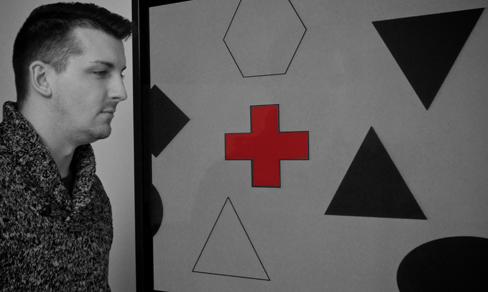
\includegraphics[scale=1.5]{perception1.jpg}
\caption{Nearly one third of participants in a study did not notice that a red cross passed on the screen because their attention was focused on the black or white figures. (credit: Cory Zanker)}
\label{fig:perception1} % Unique label used for referencing the figure in-text
%\addcontentsline{toc}{figure}{Figure \ref{fig:placeholder}} % Uncomment to add the figure to the table of contents
\end{figure}

Motivation can also affect perception. Have you ever been expecting a really important phone call and, while taking a shower, you think you hear the phone ringing, only to discover that it is not? If so, then you have experienced how motivation to detect a meaningful stimulus can shift our ability to discriminate between a true sensory stimulus and background noise. The ability to identify a stimulus when it is embedded in a distracting background is called signal detection theory. This might also explain why a mother is awakened by a quiet murmur from her baby but not by other sounds that occur while she is asleep. Signal detection theory has practical applications, such as increasing air traffic controller accuracy. Controllers need to be able to detect planes among many signals (blips) that appear on the radar screen and follow those planes as they move through the sky. In fact, the original work of the researcher who developed signal detection theory was focused on improving the sensitivity of air traffic controllers to plane blips (Swets, 1964).

Our perceptions can also be affected by our beliefs, values, prejudices, expectations, and life experiences. As you will see later in this chapter, individuals who are deprived of the experience of binocular vision during critical periods of development have trouble perceiving depth (Fawcett, Wang, \& Birch, 2005). The shared experiences of people within a given cultural context can have pronounced effects on perception. For example, Marshall Segall, Donald Campbell, and Melville Herskovits (1963) published the results of a multinational study in which they demonstrated that individuals from Western cultures were more prone to experience certain types of visual illusions than individuals from non-Western cultures, and vice versa. One such illusion that Westerners were more likely to experience was the M\"{u}ller-Lyer illusion (Figure \ref{fig:mullerlyer}): The lines appear to be different lengths, but they are actually the same length.

\begin{figure}[ht]
\centering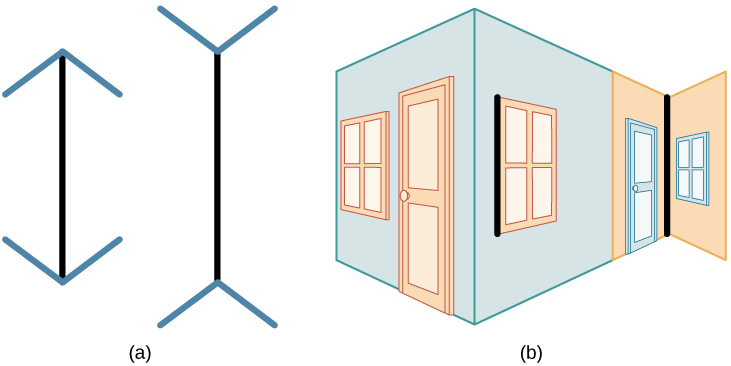
\includegraphics[scale=1]{mullerlyer.jpg}
\caption{ In the M\"{u}ller-Lyer illusion, lines appear to be different lengths although they are identical. (a) Arrows at the ends of lines may make the line on the right appear longer, although the lines are the same length. (b) When applied to a three-dimensional image, the line on the right again may appear longer although both black lines are the same length.}
\label{fig:mullerlyer} % Unique label used for referencing the figure in-text
%\addcontentsline{toc}{figure}{Figure \ref{fig:placeholder}} % Uncomment to add the figure to the table of contents
\end{figure}

These perceptual differences were consistent with differences in the types of environmental features experienced on a regular basis by people in a given cultural context. People in Western cultures, for example, have a perceptual context of buildings with straight lines, what Segall’s study called a carpentered world (Segall et al., 1966). In contrast, people from certain non-Western cultures with an uncarpentered view, such as the Zulu of South Africa, whose villages are made up of round huts arranged in circles, are less susceptible to this illusion (Segall et al., 1999). It is not just vision that is affected by cultural factors. Indeed, research has demonstrated that the ability to identify an odor, and rate its pleasantness and its intensity, varies cross-culturally (Ayabe-Kanamura, Saito, Distel, Martínez-G\'{o}mez, \& Hudson, 1998).

Children described as thrill seekers are more likely to show taste preferences for intense sour flavors (Liem, Westerbeek, Wolterink, Kok, \& de Graaf, 2004), which suggests that basic aspects of personality might affect perception. Furthermore, individuals who hold positive attitudes toward reduced-fat foods are more likely to rate foods labeled as reduced fat as tasting better than people who have less positive attitudes about these products (Aaron, Mela, \& Evans, 1994).
%------------------------------------------------
\newpage
%%----------------------------------------------------------------------------------------
%	The Perceptron CHAPTER 
%----------------------------------------------------------------------------------------
\chapterimage{ChapterCover.pdf} % Chapter heading image
\chapter{Feature Processing in Visual Cortex}

\epigraph{\textit{The only thing worse than being blind is having sight but no vision.}}{\rightline{{\rm --- \href{https://www.womenshistory.org/education-resources/biographies/helen-keller}{Helen Keller}}}}

\minitoc
\newpage
\section{Introduction to Visual Feature Processing}
Feature detection in the visual system begins with specialized neural mechanisms that extract basic visual elements from incoming sensory information. These mechanisms operate through parallel processing channels that simultaneously analyze different aspects of the visual scene, including orientation, spatial frequency, motion, and contrast.

Visual processing begins at the retina, where specialized photoreceptors convert light into neural signals. This initial stage implements fundamental processing principles through center-surround receptive fields, which enhance local contrast detection. The retinal ganglion cells perform the first stage of feature extraction, responding selectively to differences in light intensity across their receptive fields.

From the retina, visual information travels through the lateral geniculate nucleus (LGN) to the primary visual cortex (V1), where more sophisticated feature detection begins. In V1, simple cells respond to oriented edges and lines at specific positions in their receptive fields, acting as basic feature detectors. These cells implement a form of spatial filtering, effectively decomposing the visual scene into its fundamental components of orientation and spatial frequency.
\begin{wrapfigure}{R}{0.6\textwidth}
\begin{tcolorbox}[every float=\centering, drop shadow, title=Organization of the Retina ,colback=white,colframe=WMgreen,
  colbacktitle=WMgreen,]
 \begin{tikzpicture}
  % Nodes for layers
  \node[draw, circle, fill=red!50] (P1) at (0, 4) {};
  \node[draw, circle, fill=red!50] (P2) at (1, 4) {};
  \node[draw, circle, fill=red!50] (P3) at (2, 4) {};
  \node[draw, circle, fill=red!50] (P4) at (3, 4) {};

  %\node[draw, circle, fill=green!50] (H1) at (0.5, 3) {};
  \node[draw, ellipse, minimum width=2cm, minimum height=.2cm, fill=green!50] (H1) at (.7,3) {};
  \node[draw, ellipse, minimum width=2cm, minimum height=.2cm, fill=green!50] (H2) at (2.3,3) {};
  %\node[draw, circle, fill=green!50] (H2) at (2.5, 3) {};

  \node[draw, circle, fill=blue!50] (B1) at (0.5, 2) {};
  \node[draw, circle, fill=blue!50] (B2) at (2.5, 2) {};

 \node[draw, ellipse, minimum width=2cm, minimum height=.2cm, fill=orange!50] (A1) at (.7,1) {};
  \node[draw, ellipse, minimum width=2cm, minimum height=.2cm, fill=orange!50] (A2) at (2.3,1) {};
 % \node[draw, circle, fill=orange!50] (A1) at (0, 1) {};
  %\node[draw, circle, fill=orange!50] (A2) at (1, 1) {};
  %\node[draw, circle, fill=orange!50] (A3) at (2, 1) {};
  %\node[draw, circle, fill=orange!50] (A4) at (3, 1) {};

  \node[draw, circle, fill=purple!50] (G1) at (1.5, 0) {};

  % Connections
  \foreach \i in {P1,P2,P3,P4} {
    \foreach \j in {H1,H2} {
      \draw[thin] (\i) -- (\j);
    }
  }

  \foreach \i in {H1,H2} {
    \foreach \j in {B1,B2} {
      \draw[thin] (\i) -- (\j);
    }
  }

  \foreach \i in {B1,B2} {
    \foreach \j in {A1,A2} {
      \draw[thin] (\i) -- (\j);
    }
  }

  \foreach \i in {A1,A2} {
    \draw[thin] (\i) -- (G1);
  }

  % Labels
  \node[align=left] at (5, 4) {\textbf{Photoreceptors}};
  \node[align=left] at (5, 3) {\textbf{Horizontal Cells}};
  \node[align=left] at (5, 2) {\textbf{Bipolar Cells}};
  \node[align=left] at (5, 1) {\textbf{Amacrine Cells}};
  \node[align=left] at (5, 0) {\textbf{Ganglion Cells}};
  \node[align=left] at (5, -1) {\textbf{Optic Nerve}};
  \node[align=left] at (5,-2) {\textbf{Receptive Field}};

  % Light rays
  \draw[blue, very thick, ->] (-1.5, 4) -- (-1.5, -2);
   \node[rotate=270, anchor=south] at (-1.5,1) {Signaling};
    %signaling
   \draw[yellow, very thick, ->] (-2, -2) -- (-2, 4);
   \node[rotate=90, anchor=north] at (-2.6,1) {Light};
  %\draw[yellow, very thick, ->] (-0.5, 5) -- (0, 4.5);
  %\draw[yellow, very thick, ->] (0, 5) -- (0.5, 4.5);

  %optic nerve
  \draw[black, very thick, ->] (1.5,0) -- (1.5, -1.5);
  
  %RF
  \node[draw, ellipse, minimum width=2.5cm, minimum height=.6cm, fill=blue!30] (rfsurround) at (1.5,-2) {};
    \node[draw, ellipse, minimum width=1.5cm, minimum height=.2cm, fill=blue] (rfcenter) at (1.5,-2) {};
\end{tikzpicture}
 \captionof{figure}{Organization of the cells of the retina.  Signaling initiated by the photoreceptors is filtered by a network of horizontal, bipolar, and amacrine cells as it is passed to the retinal ganglion cells, resulting in their center-surround receptive fields}
  \label{fig:retina}
 \end{tcolorbox}
 \end{wrapfigure}

As information flows through higher visual areas (V2, V3, V4, etc.), the processing becomes progressively more sophisticated. Simple cells in V1 converge onto complex cells that respond to oriented edges regardless of exact position, demonstrating how the system builds invariant representations. This hierarchical convergence continues through the ventral visual stream, where neurons become selective for increasingly complex features - from simple edges in V1, to contours and shapes in V2 and V3, to object parts in V4, and finally to whole objects in inferior temporal cortex. This organization reflects a fundamental principle of neural computation where simpler features are progressively combined to represent more complex visual attributes, allowing the brain to efficiently process and understand visual scenes.

\section{Retinal Filtering}
The retina plays a crucial role in the early stages of visual processing, performing complex computations on incoming visual information before it reaches the brain. This preprocessing in the retina allows for efficient and rapid analysis of visual scenes by extracting key features and distributing information across parallel channels.
\clearpage
\begin{wrapfigure}{R!}{0.4\textwidth}
\begin{tcolorbox}[every float=\centering, drop shadow, title=Mach Band Effect ,colback=white,colframe=WMgreen,
  colbacktitle=WMgreen,]
 \begin{tikzpicture}[scale=1.2]
    % Create gradient bars with decreasing darkness (4 bars only)
    \foreach \x in {0,1,2,3} {
        \fill[gray!\the\numexpr 100-\x*25\relax] (\x,0) rectangle (\x+1,2);
    }
    
    % Draw actual intensity step function (directly over bars)
    \draw[thick, blue] (0,0) -- (1,0)
                 (1,0) -- (1,0.5) -- (2,0.5)
                 (2,0.5) -- (2,1.0) -- (3,1.0)
                 (3,1.0) -- (3,1.5) -- (4,1.5);
    
    % Draw perceived intensity with brief transitions (over bars)
    \draw[very thick, red] (0,0) -- (0.8,0)
                 (0.8,0) .. controls (0.94,0.4) and (1.1,-.65) .. (1.1,0.5)
                 (1.2,0.5) -- (1.8,0.5)
                 (1.8,0.5) .. controls (1.94,0.9) and (2.1,-0.15) .. (2.1,1.0)
                 (2.2,1.0) -- (2.8,1.0)
                 (2.8,1.0) .. controls (2.94,1.4) and (3.1,0.35) .. (3.1,1.5)
                 (3.2,1.5) -- (4,1.5);
    
    % Add labels
% Add legend below the bars
\draw[very thick, blue] (0,-0.5) -- (0.5,-0.5) node[right] {Actual Intensity};
\draw[very thick, red] (0,-1) -- (0.5,-1) node[right] {Perceived Intensity};
\end{tikzpicture}
 \captionof{figure}{Illustration of the Mach band effect.}
  \label{fig:MachBand}
 \end{tcolorbox}
 \end{wrapfigure}
 
The retina is composed of several layers of specialized neurons that work together to process visual input. When light enters the eye, it activates photoreceptors (rods and cones) in the outermost layer of the retina. These photoreceptors convert light into electrical signals, which are then passed through a network of bipolar cells, horizontal cells, amacrine cells, and ultimately to retinal ganglion cells (RGCs). Each of these cell types contributes to specific aspects of visual processing: Photoreceptors: Rods are responsible for scotopic (low-light) vision, while cones mediate photopic (bright-light) vision and color perception. Horizontal cells: These cells create lateral connections between photoreceptors and bipolar cells, enhancing contrast and sharpening edges in the visual scene. Bipolar cells: They relay signals from photoreceptors to RGCs, with some types responding to increases in light (ON bipolar cells) and others to decreases (OFF bipolar cells). Amacrine cells: These interneurons modulate the activity of bipolar cells and RGCs, contributing to motion detection and other complex visual features.
Retinal ganglion cells: RGCs are the output neurons of the retina, sending visual information to the brain via their axons, which form the optic nerve.
\begin{wrapfigure}{L!}{0.6\textwidth}
\begin{tcolorbox}[every float=\centering, drop shadow, title=Lateral Inhibition ,colback=white,colframe=WMgreen,
  colbacktitle=WMgreen,]
\begin{tikzpicture}[scale=.7]
    % Parameters
    \def\barwidth{1.0}
    \def\barheight{3.0}
    \def\spacing{0.1}

    % Luminance values
    \def\Lzero{0.2}
    \def\Lone{0.2}
    \def\Ltwo{0.2}
    \def\Lthree{.8}
    \def\Lfour{0.2}
    \def\Lfive{0.2}
    \def\Lsix{0.2}

    % Calculated perceived luminance
    \pgfmathsetmacro{\Pzero}{round((\Lzero - 0.2*(\Lone))*100)/100}
   \pgfmathsetmacro{\Pone}{round(max(\Lone - 0.2*(\Ltwo + \Lzero), 0)*100)/100}
    \pgfmathsetmacro{\Ptwo}{round(max(\Ltwo- 0.2*(\Lone + \Lthree), 0)*100)/100}
    \pgfmathsetmacro{\Pthree}{round((\Lthree - 0.2*(\Ltwo + \Lfour))*100)/100}
    \pgfmathsetmacro{\Pfour}{round(max(\Lfour - 0.2*(\Lthree + \Lfive), 0)*100)/100}
    \pgfmathsetmacro{\Pfive}{round(max(\Lfive - 0.2*(\Lfour + \Lsix), 0)*100)/100}
    \pgfmathsetmacro{\Psix}{round(max(\Lsix - 0.2*(\Lfive), 0)*100)/100}

    % Draw original luminance bars
    \foreach \i/\Lum in {0/\Lzero, 1/\Lone, 2/\Ltwo, 3/\Lthree, 4/\Lfour, 5/\Lfive, 6/\Lsix} {
        \pgfmathsetmacro{\grayvalue}{100-\Lum*100}
        \fill[gray!\grayvalue] (\i*\barwidth+\i*\spacing, 0) rectangle ++(\barwidth, \barheight);
        \node[above] at (\i*\barwidth+\i*\spacing+0.5*\barwidth, \barheight){\footnotesize{\pgfmathprintnumber[fixed, precision=1]{\Lum}}}; % {$\Lum$};
    }

    % Draw lateral inhibition curves
    \foreach \i in {0,...,5} {
        \pgfmathsetmacro{\startx}{\i*\barwidth+\i*\spacing+0.5*\barwidth}
        \pgfmathsetmacro{\endx}{(\i+1)*\barwidth+(\i+1)*\spacing+0.5*\barwidth}
        \draw[red, ->] (\startx, 0) .. controls (\startx, -1) and (\endx, -1) .. (\endx, 0);
        \draw[red, ->] (\endx, 0) .. controls (\endx, -1) and (\startx, -1) .. (\startx, 0);
    }

    % Draw perceived luminance bars
    \foreach \i/\Perc in {0/\Pzero, 1/\Pone, 2/\Ptwo, 3/\Pthree, 4/\Pfour, 5/\Pfive, 6/\Psix} {
        \pgfmathsetmacro{\grayvalue}{100-\Perc*100}
        \fill[gray!\grayvalue] (\i*\barwidth+\i*\spacing, -4) rectangle ++(\barwidth, \barheight);
        \node[below] at (\i*\barwidth+\i*\spacing+0.5*\barwidth, -4) {\footnotesize{\pgfmathprintnumber[fixed, precision=2]{\Perc}}}; %{$\Perc$};
    }

    % Labels
    \node[left] at (-.2, 1.5) {\small{Actual Luminance}};
    \node[left] at (-.2, -2.5) {\small{Perceived Luminance}};
    

    % Title
   % \node[above] at (3*\barwidth+3*\spacing, 4) {\textbf{Effect of Lateral Inhibition on Contrast}};
    
    % Mathematical model
    %\node[right] at (7.5, -1) {
     %   \begin{tabular}{l}
      %      \textbf{Mathematical Model:} \\
      %      $P_i = \max(L_i - k(L_{i-1} + L_{i+1}), 0)$ \\
        %    where: \\
          %  $P_i$: Perceived luminance \\
         %   $L_i$: Original luminance \\
           % $k$: Inhibition strength (0.1) \\
        %\end{tabular}
   % };
\end{tikzpicture}
 \captionof{figure}{\small{Illustration of how uniform lateral inhibition works to increase contrast at boundaries. This model assumes that the perceived luminance value in the receptive field for RGC $i$, $P_i$, is simply the actual luminance, $L_i$, minus the inhibition by its immediate neighbors, which is a proportion, $k$, of the their actual luminance. In other words, we use the actual luminance values to compute the perceived luminance for each of the RGCs pictured so that $P_i=L_i-k(L_i-1 + L_i+1)$.  The example illustrates the model with $k=2$.}}
  \label{fig:LatInhibition}
 \end{tcolorbox}
\end{wrapfigure}

One of the key functions of retinal processing is to perform early filtering of visual information. This filtering begins with the center-surround organization of RGC receptive fields. Each RGC responds most strongly to light hitting a small region in the center of its receptive field, with the surrounding area having an opposing effect. This organization allows for the detection of local contrast and edges through lateral inhibition, which enhances contrast sensitivity by suppressing uniform regions while amplifying differences at edges. This is evident in phenomena like the Mach band effect, where lateral inhibition creates exaggerated brightness transitions at edges.

Lateral inhibition in the retina creates the fundamental building blocks for visual processing through the establishment of center-surround receptive fields for the RGC. The center-surround organization of RGC receptive fields emerges through a complex interplay of neural circuits operating at multiple levels. Light information from photoreceptors first synapses onto ON and OFF bipolar cells, which respond oppositely to glutamate released by photoreceptors. ON bipolar cells are activated by light (inhibited by glutamate), while OFF bipolar cells are inhibited by light (excited by glutamate). These bipolar cells then connect to retinal ganglion cells in a parallel pathway, maintaining the ON/OFF organization. When light hits the center of a ganglion cell's receptive field, it can either excite the cell through ON bipolar cells or inhibit it through OFF bipolar cells, creating ON-center or OFF-center ganglion cells respectively. 
\begin{figure}[h!]
\begin{tcolorbox}[every float=\centering, drop shadow, title=Center-Surround Receptive Fields ,colback=white,colframe=WMgreen,
  colbacktitle=WMgreen,]
 \begin{tikzpicture}
%Receptive Fields
  %whole RF
  \fill[yellow!30] (15,3) circle (.9);
  
\foreach \x in {6,9,12,15} {
        \fill[blue!30] (\x,3) circle (0.7);
        \fill[blue] (\x,3) circle (0.4);
    }
    \node [align=center] at (6,4.4) {Baseline \\ (No stimulus)};
     \node [align=center] at (9,4.4) {On-center \\ stimulated};
     \node [align=center] at (12,4.4) {Off-surround \\ stimulated};
     \node [align=center] at (15,4.4) {Full RF \\ stimulated};
  %Baseline activation
  \draw[thick] (4.6,1.2) -- (7.4,1.2);
  \draw[thick] (4.6,1.2) -- (4.6,1.4);
  \draw[thick] (7.4,1.2) -- (7.4,1.4);
  \draw[thin](4.8,1.2)--(4.8,1.7);
 % \draw[thin](5.3,1.2)--(5.3,1.7);
  \draw[thin](5.9,1.2)--(5.9,1.7);
  \draw[thin](6.5,1.2)--(6.5,1.7);
  \draw[thin](7,1.2)--(7,1.7);
  %On center
  \draw[thick] (7.6,1.2) -- (10.4,1.2);
  \draw[thick] (7.6,1.2) -- (7.6,1.4);
  \draw[thick] (10.4,1.2) -- (10.4,1.4);
  \draw[thin](9.4,1.2)--(9.4,1.7);
  \draw[thin](9.6,1.2)--(9.6,1.7);
  \draw[thin](7.9,1.2)--(7.9,1.7);
  \draw[thin](8.1,1.2)--(8.1,1.7);
  \draw[thin](8.2,1.2)--(8.2,1.7);
  \draw[thin](8.3,1.2)--(8.3,1.7);
  \draw[thin](8.5,1.2)--(8.5,1.7);
  \draw[thin](8.7,1.2)--(8.7,1.7);
  \draw[thin](8.8,1.2)--(8.8,1.7);
  \draw[thin](9.1,1.2)--(9.1,1.7);
  \draw[thin](9.2,1.2)--(9.2,1.7);
  \draw[thin](9.3,1.2)--(9.3,1.7);
  \draw[thin](9.8,1.2)--(9.8,1.7);
  \draw[thin](9.9,1.2)--(9.9,1.7);
  \draw[thin](10.1,1.2)--(10.1,1.7);
  %Off surround
  \draw[thick] (10.6,1.2) -- (13.4,1.2);
  \draw[thick] (10.6,1.2) -- (10.6,1.4);
  \draw[thick] (13.4,1.2) -- (13.4,1.4);
  \draw[thin](12.3,1.2)--(12.3,1.7);
  %full RF
  %Baseline activation
  \draw[thick] (13.6,1.2) -- (16.4,1.2);
  \draw[thick] (13.6,1.2) -- (13.6,1.4);
  \draw[thick] (16.4,1.2) -- (16.4,1.4);
  \draw[thin](13.8,1.2)--(13.8,1.7);
  \draw[thin](14.3,1.2)--(14.3,1.7);
  \draw[thin](14.9,1.2)--(14.9,1.7);
  \draw[thin](15.2,1.2)--(15.2,1.7);
  \draw[thin](15.5,1.2)--(15.5,1.7);
  \draw[thin](15.7,1.2)--(15.7,1.7);
  \draw[thin](16,1.2)--(16,1.7);
  %center fill
  \fill[yellow!30] (9,3) circle (0.4);
  %surround fill
  \fill[yellow!30] (12,3) circle (0.7);
  \fill[blue] (12,3) circle (0.4);
 %whole RF
 \fill[yellow!30, fill opacity=.3] (15,3) circle (.7);
  %Row labels
  \node[left] at (4,3) {Receptive Fields};
  \node[left] at (4,1.5) {RGC Activity};
 %legend
 \fill[yellow!30] (4,3.8) rectangle (4.4,4.3);
 \node[left] at (4,4) {Light Stimulus};
 \end{tikzpicture}
  \captionof{figure}{Responses by on-center retinal ganglion cells (RCGs) following various light stimuli.  The baseline represents the baseline firing rate of the RCG when no light stimulus is present.  the RCG is maximally activated when the light stimulus fall only on the on-center region of the RF.  Similarly, the RCG is maximally suppressed when only the off-surround is stimulated by light.  Finally, if the light stimulus covered both the on-center and off-surround, only a slight increase in activity from baseline may be observed.}
  \label{fig:OnCenterRFs}
 \end{tcolorbox}
\end{figure}
 
 In the outer retina, photoreceptors make excitatory connections to bipolar cells, creating the "center" response. These same photoreceptors also connect to horizontal cells, which spread the signal laterally and provide inhibitory feedback to neighboring photoreceptors. This horizontal cell feedback creates an initial antagonistic surround effect, where stimulation of the surrounding area produces the opposite response to stimulation of the center. The inner retina adds another layer of lateral inhibition through amacrine cells, which further refine the center-surround organization. The system effectively compares the light falling on one area of the retina with the light falling on adjacent areas, making cells particularly responsive to differences in illumination between the center and surround regions.

These ON and OFF pathways remain segregated as the information travels through the lateral geniculate nucleus (LGN) to V1, where multiple center-surround units are combined to create more complex receptive fields like edge detectors. The parallel processing of ON and OFF information allows the visual system to efficiently encode both light increments and decrements. The retina also performs parallel processing of different visual properties. Different types of RGCs extract specific features from the visual scene, such as luminance, local contrast, spatial and temporal frequency, motion, motion direction, and color. This parallel processing enables the brain to analyze visual information rapidly and efficiently based on these pre-extracted features.

By performing these complex computations and filtering operations, the retina significantly reduces the amount of raw visual data that needs to be transmitted to and processed by the brain. This preprocessing allows higher-level visual areas to focus on more complex tasks such as object recognition, motion analysis, and scene interpretation.

\section{Simple Cells \& Orientation Selectivity}
Simple cells in the primary visual cortex (V1) play a crucial role in early visual processing, particularly in orientation selectivity and edge detection. These neurons, first described by David Hubel and Torsten Wiesel, have elongated receptive fields with distinct excitatory and inhibitory regions arranged in parallel12. This unique structure allows simple cells to respond selectively to oriented stimuli, such as bars or edges with specific orientations in their receptive fields.

The orientation selectivity of simple cells arises from the convergence of inputs from lateral geniculate nucleus (LGN) cells. According to Hubel and Wiesel's model, several LGN cells with center-surround receptive fields are arranged in a line, forming the elongated structure of a simple cell's receptive field2. This arrangement results in a narrow receptive field for the simple cell, with its preferred orientation aligned with the arrangement of LGN inputs1.
\begin{wrapfigure}{L!}{0.4\textwidth}
\begin{tcolorbox}[every float=\centering, drop shadow, title=Simple Cells in V1 ,colback=white,colframe=WMgreen,
  colbacktitle=WMgreen,]

\begin{tikzpicture}[scale=1.2]
    
    % Part B: V1 Integration
    % Title for Part B
    % Center-surround receptive fields
    \foreach \x in {-.8,-.5,-.2,.1,.4,.7} {
        \fill[blue!30] (\x,3) circle (0.4);
    }
    \foreach \x in {-.8,-.5,-.2,.1,.4,.7}{
       \fill[blue] (\x,3) circle (0.2);
    }
   % \node at (7,3.5) {Center-Surround Fields}; 
    % V1 neuron
    \fill[purple] (-.5,.5) rectangle (.5,1.5);
    \node at (0,0) {V1 Neuron};
    
    % Connections to V1
    \foreach \x in {-.8,-.5,-.2,.1,.4,.7} {
        \draw[dashed] (\x,3) -- (0,1.5);
    }
    
    %start of angle v1
     \foreach \x/\y in {1.8/2.4,2.1/2.6,2.4/2.8,2.7/3,3/3.2,3.3/3.4} {
        \fill[blue!30] (\x,\y) circle (0.4);
    }
     \foreach \x/\y in  {1.8/2.4,2.1/2.6,2.4/2.8,2.7/3,3/3.2,3.3/3.4} {
       \fill[blue] (\x,\y) circle (0.2);
    }
   % \node at (7,3.5) {Center-Surround Fields}; 
    % V1 neuron
    \fill[purple] (2.4,.5) rectangle (3.4,1.5);
    \node at (2.8,0) {V1 Neuron};
    
    % Connections to V1
    \foreach \x/\y in  {1.8/2.4,2.1/2.6,2.4/2.8,2.7/3,3/3.2,3.3/3.4} {
        \draw[dashed] (\x,\y) -- (2.9,1.5);
    }
\end{tikzpicture}
  \captionof{figure}{Illustration of how the convergence of RGC receptive fields on V1 neurons can produce edge detectors.}
  \label{fig:SimpleCells}
 \end{tcolorbox}
\end{wrapfigure}

Simple cells play a crucial role in spatial frequency analysis of visual information. These neurons, first described by Hubel and Wiesel, have elongated receptive fields with distinct excitatory and inhibitory regions arranged in parallel. This unique structure allows simple cells to act as spatial frequency filters, responding selectively to specific spatial frequencies in their receptive fields. 

Spatial frequency is a fundamental concept in visual perception and image processing that describes how rapidly brightness or color changes across space in an image or visual scene. It is typically measured in cycles per degree of visual angle or cycles per unit distance (e.g., cycles per millimeter).

The spatial frequency selectivity of simple cells arises from the organization of their receptive fields. The width of the excitatory and inhibitory subregions in a simple cell's receptive field corresponds closely to the spatial frequency to which the cell responds most strongly1. This relationship between receptive field structure and spatial frequency tuning suggests that simple cells perform a local Fourier analysis of the visual scene.

Simple cells exhibit a range of preferred spatial frequencies, typically spanning from 0.2 to 2.0 cycles per degree in cats8. This diversity allows the visual system to analyze different scales of spatial information in parallel. Importantly, the spatial frequency selectivity of simple cells is often sharper than that of their inputs from the lateral geniculate nucleus (LGN), indicating that cortical mechanisms enhance and refine spatial frequency tuning4.

The responses of simple cells to sinusoidal gratings can be predicted remarkably well from their spatial receptive fields2. This quasi-linear behavior extends to more complex stimuli, including natural scenes. However, there is evidence of nonlinear mechanisms that further shape spatial frequency selectivity, particularly in the suppression of responses to non-preferred spatial frequencies.

\begin{wrapfigure}{R!}{0.5\textwidth}
\begin{tcolorbox}[every float=\centering, drop shadow, title=Concept of Spatial Frequency ,colback=white,colframe=WMgreen,
  colbacktitle=WMgreen,]
\begin{tikzpicture}[scale=.7]

% Low spatial frequency sinusoidal pattern
\foreach \x in {0, 0.5, ..., 10} {
    \draw[thick] (\x, 4) -- ++(0, 0.5);
    \draw[thick] (\x+0.25, 4) -- ++(0, -0.5);
}
\node[above] at (5, 4.5) {Low Spatial Frequency};

% Medium spatial frequency sinusoidal pattern
\foreach \x in {0, 0.25, ..., 10} {
    \draw[thick] (\x, 2) -- ++(0, 0.5);
    \draw[thick] (\x+0.125, 2) -- ++(0, -0.5);
}
\node[above] at (5, 2.5) {Medium Spatial Frequency};

% High spatial frequency sinusoidal pattern
\foreach \x in {0, 0.125, ..., 10} {
    \draw[thick] (\x, 0) -- ++(0, 0.5);
    \draw[thick] (\x+0.0625, 0) -- ++(0, -0.5);
}
\node[above] at (5, 0.5) {High Spatial Frequency};

\end{tikzpicture}
 \captionof{figure}{Illustration of stimuli with low, medium, and high spatial frequency.}
  \label{fig:spatialfrequency}
 \end{tcolorbox}
\end{wrapfigure}
\FloatBarrier

Interestingly, adjacent simple cells in V1 often have similar spatial frequency and orientation preferences but differ in their spatial phase. This arrangement suggests that groups of simple cells may function as quadrature pairs, effectively implementing sine and cosine filters for a given spatial frequency and orientation7. Such an organization would allow the visual system to encode both the magnitude and phase of spatial frequency components in the visual scene.

The spatial frequency analysis performed by simple cells contributes to various aspects of visual processing, including edge detection, texture analysis, and the initial stages of object recognition. By decomposing the visual scene into its constituent spatial frequencies, simple cells provide a foundation for more complex visual computations in higher cortical areas.

\section{Gabor Filters}
Gabor filters are powerful tools in image processing and computer vision, serving as spatial filters that can extract important features from images. Named after Dennis Gabor, these filters are particularly effective at analyzing textures, detecting edges, and extracting features that are, not unlike simple cells in V1, sensitive to both frequency and orientation information in images.

The Gabor filter is essentially a Gaussian kernel function modulated by a sinusoidal plane wave. In the spatial domain, it can be represented mathematically as: $G(x,y)=\exp{-\frac{x^2+y^2}{2}}\cdot cos(2\pi x)$.

Gabor filters are particularly useful because they can capture local spatial and frequency information simultaneously. This property makes them well-suited for texture analysis, edge detection, and feature extraction in various computer vision applications.

\begin{wrapfigure}{L}{0.4\textwidth}
\begin{tcolorbox}[every float=\centering, drop shadow, title=The Gabor Kernel Function ,colback=white,colframe=WMgreen,
  colbacktitle=WMgreen,]
\begin{tikzpicture}[scale=.6]
    \begin{axis}[
        axis lines=none, % Simplifies the plot by removing axis lines
        width=10cm, % Sets the width of the plot
        domain=-4:4, % Range for x
        y domain=-4:4, % Range for y
        samples=50, % Number of samples for x
        samples y=50, % Number of samples for y
        colormap/bluered, % Color scheme: blue (small) to red (large)
        view={0}{90}, % Top-down 2D view
        colorbar, % Adds a colorbar for intensity scale
        point meta min=-1, % Minimum value for color scaling
        point meta max=1 % Maximum value for color scaling
    ]
        % Gabor kernel equation
        \addplot3[
            surf,
            shader=interp % Smooth interpolation for surface
        ]
        {exp(-0.5*(x^2 + y^2)) * cos(deg(2*3.14159*x))};
    \end{axis}
\end{tikzpicture}
 \captionof{figure}{2-dimensional Illustration of a Gabor kernel.}
  \label{fig:gabor}
 \end{tcolorbox}
\end{wrapfigure}
\FloatBarrier

One of the key advantages of Gabor filters is their similarity to the human visual system's processing of visual information. The filters' frequency and orientation representations are similar to those of the human visual cortex, making them biologically inspired and effective for mimicking human perception in computer vision tasks35. By varying parameters such as frequency, orientation, and bandwidth, we can create a bank of Gabor filters that can extract a rich set of features from an image.

When applied to an image through convolution, Gabor filters can highlight different texture characteristics and orientations. For example, by using Gabor filters with different orientations, we can detect edges and lines in various directions within an image. Similarly, by adjusting the frequency parameter, we can extract features at different scales, allowing for the analysis of both fine and coarse textures. The features extracted using Gabor filters can be used in various machine learning tasks, such as texture classification, object recognition, and image segmentation. 

Convolution is a fundamental operation in image processing and computer vision that involves sliding a small matrix, called a kernel or filter, over an input image to produce a new output image. The process works by multiplying each pixel in the input image by the corresponding value in the kernel, summing the results, and placing this sum in the corresponding position of the output image. This operation allows for various image transformations, including blurring, sharpening, and edge detection, depending on the values in the kernel.

\begin{figure}[h!]
\centering
\begin{tcolorbox}[every float=\centering, drop shadow, title=Image Filtering by Convolution ,colback=white,colframe=WMgreen,
  colbacktitle=WMgreen,]
  \centering
\begin{tikzpicture}[
    2d-arr/.style={matrix of nodes, row sep=-\pgflinewidth, column sep=-\pgflinewidth, nodes={draw, minimum size=0.6cm}},
    pixel/.style={fill=black!#1, text=blue}
]

% Input image (letter T)
\matrix (input) [2d-arr] {
    |[pixel=0]| 0 & |[pixel=0]| 0 & |[pixel=0]| 0 & |[pixel=60]| 1 & |[pixel=0]| 0 & |[pixel=0]| 0 & |[pixel=0]| 0\\
    |[pixel=0]| 0 & |[pixel=0]| 0 & |[pixel=0]| 0 & |[pixel=60]| 1 & |[pixel=0]| 0 & |[pixel=0]| 0 & |[pixel=0]| 0\\
    |[pixel=60]| 1 & |[pixel=60]| 1 & |[pixel=60]| 1 & |[pixel=60]| 1 & |[pixel=60]| 1 & |[pixel=60]| 1 & |[pixel=60]| 1\\
    |[pixel=0]| 0 & |[pixel=0]| 0 & |[pixel=0]| 0 & |[pixel=60]| 1 & |[pixel=0]| 0 & |[pixel=0]| 0 & |[pixel=0]| 0\\
    |[pixel=0]| 0 & |[pixel=0]| 0 & |[pixel=0]| 0 & |[pixel=60]| 1 & |[pixel=0]| 0 & |[pixel=0]| 0 & |[pixel=0]| 0\\
    |[pixel=0]| 0 & |[pixel=0]| 0 & |[pixel=0]| 0 & |[pixel=60]| 1 & |[pixel=0]| 0 & |[pixel=0]| 0 & |[pixel=0]| 0\\
    |[pixel=0]| 0 & |[pixel=0]| 0 & |[pixel=0]| 0 & |[pixel=60]| 1 & |[pixel=0]| 0 & |[pixel=0]| 0 & |[pixel=0]| 0\\
};
\node[below=of input-6-4] {Input Image};

% Convolution operator
\node[right=0.5cm of input] (conv) {$*$};

% Kernel (edge detection)
\matrix (kernel) [2d-arr, right=0.5cm of conv, nodes={draw, minimum size=0.5cm}] {
    |[pixel=0]| 0 & |[pixel=50]| .5 & |[pixel=0]| 0 \\
    |[pixel=0]| 0 & |[pixel=750]| 1 & |[pixel=0]| 0 \\
    |[pixel=0]| 0 & |[pixel=50]| .5 & |[pixel=0]| 0 \\
};
\node[below=0.5cm of kernel-3-2] {Kernel};

% Equals sign
\node[right=0.5cm of kernel] (eq) {$=$};

% Output (edge-detected T)
\matrix (output) [2d-arr, right=0.5cm of eq] {
    |[pixel=25]| .5 & |[pixel=25]| .5 & |[pixel=100]| 2 & |[pixel=25]| .5 & |[pixel=25]| .5\\
    |[pixel=60]| 1 & |[pixel=60]| 1 & |[pixel=100]| 2 & |[pixel=60]| 1 & |[pixel=60]| 1 \\
    |[pixel=25]| .5 & |[pixel=25]| .5 & |[pixel=100]| 2 & |[pixel=25]| .5 & |[pixel=25]| .5\\
    |[pixel=0]| 0 & |[pixel=0]| 0 & |[pixel=100]| 2 & |[pixel=0]| 0 & |[pixel=0]| 0 \\
    |[pixel=0]| 0 & |[pixel=0]| 0 & |[pixel=100]| 2 & |[pixel=0]| 0 & |[pixel=0]| 0\\
};
\node[below=of output-4-3] {Output};

% Highlight convolution area
\draw[dashed, red, very thick] (input-2-3.north west) rectangle (input-4-5.south east);
\draw[dashed, blue, very thick] (output-2-3.north west) rectangle (output-2-3.south east);
\draw[<-, red, thick] (kernel-2-1) to[bend left] (input-4-5);
\draw[->, blue, thick] (kernel-2-3) to[bend right] (output-2-3);

\end{tikzpicture}
 \captionof{figure}{Illustration of the convolution operation.  Here an input image with various luminance values is filtered using a simple gabor-like kernel.  Notice how convolution with a vertically oriented gabor kernel nicely exaggerates the vertical edges, but not the horizontal edges.}
  \label{fig:convolution}
 \end{tcolorbox}
\end{figure}
\FloatBarrier

The convolution operation is particularly powerful because it can extract meaningful features from images. By using different kernels, we can emphasize various aspects of an image, such as edges, textures, or specific patterns. One type of filter that leverages convolution for feature analysis is the Gabor filter.

Research has shown that Gabor filters provide a reasonably accurate description of most spatial aspects of simple receptive fields in V1. Simple cells in the visual cortex exhibit responses that can be well-modeled by Gabor-like functions, with specific orientations, spatial frequencies, and phases1. This correspondence suggests that the visual system has evolved to efficiently extract relevant features from visual stimuli, much like Gabor filters do in image processing applications. The Gabor function's ability to simultaneously represent information in both spatial and frequency domains aligns with the visual system's need to analyze both local and global image properties2.

\begin{figure}[h!]
\centering
\begin{tcolorbox}[every float=\centering, drop shadow, title=Varying Orientation and Wavelength of the Gabor Filters ,colback=white,colframe=WMgreen,
  colbacktitle=WMgreen,]
  \centering
\begin{tikzpicture}[scale=2]
    \foreach \freq/\angle in {0.5/0, 1.0/45, 1.5/90}{
        \begin{scope}[shift={(\freq*4cm,0)}]
            \begin{axis}[
                axis lines=none,
                width=3cm,
                domain=-3:3,
                y domain=-3:3,
                samples=40,
                samples y=40,
                colormap/bluered,
                view={0}{90}
            ]
                \addplot3[surf, shader=interp]
                {exp(-0.5*(x^2 + y^2)) * 
                 cos(deg(2*pi*(\freq*(x*cos(\angle) + y*sin(\angle)))))};
            \end{axis}
        \end{scope}
    }
\end{tikzpicture}
 \captionof{figure}{Illustration of various gabor filters with decreasing wavelength ($\lambda$) and increasing angle of rotation from left to right.}
  \label{fig:gaborangles}
 \end{tcolorbox}
\end{figure}
\FloatBarrier

However, it's important to note that while Gabor filters provide a good approximation of simple cell responses, they do not capture the full complexity of neural processing in V1. Recent studies using convolutional neural networks (CNNs) have suggested that V1 neurons may involve more nonlinear computations than previously thought. Nonetheless, even in these more complex models, Gabor-like filters often emerge in the early layers, indicating their fundamental importance in visual processing. The relationship between Gabor filters and neural responses underscores the biological inspiration behind many computer vision algorithms and highlights the efficiency of the visual system in extracting meaningful information from the environment.

The output from convolving an image with a Gabor filter provides valuable information about the texture and edge characteristics of the image at specific orientations and frequencies. Here's how to interpret this output:

\begin{itemize}
    \item Magnitude Response
The magnitude of the Gabor filter output indicates the strength of the texture or edge features in the image that match the filter's parameters:
High magnitude values correspond to areas in the image where there is a strong presence of features (such as edges or textures) that align with the filter's orientation and frequency. Low magnitude values indicate regions where such features are absent or weak.
    \item Interpretation Based on Filter Parameters
The interpretation of the output depends on the specific parameters of the Gabor filter used:

Orientation ($\theta$): The output will highlight features oriented in the direction specified by $\theta$. For example, a filter with $\theta = 0\deg$ will respond strongly to horizontal features.

Wavelength ($\lambda$): This parameter determines the scale of features detected. Smaller wavelengths detect finer textures, while larger wavelengths capture coarser structures2.

Bandwidth ($\sigma$): This affects the range of frequencies the filter responds to. A larger $\sigma$ results in a broader response to a range of frequencies.

    \item Multiple Filter Responses
Often, a bank of Gabor filters with different orientations and scales is used:
By analyzing the responses across multiple filters, you can build a comprehensive representation of the image's texture and edge characteristics.
\end{itemize}

\printglossary[type=datacollection,style=twocolumn]
%\printglossary
%\glsresetall
\newpage
\bibliographystyle{apalike}
\renewcommand{\bibname}{References}
\bibliography{bibliography}


%%----------------------------------------------------------------------------------------
%	The Perceptron CHAPTER 
%----------------------------------------------------------------------------------------
\chapterimage{ChapterCover.pdf} % Chapter heading image
\chapter{The Perceptron}

\epigraph{\textit{Artificial intelligence is the science of making machines do things that would require intelligence if done by men.}}{\rightline{{\rm --- \href{https://en.wikipedia.org/wiki/Marvin_Minsky}{Marvin Minsky}}}}

\minitoc
\newpage
\section{Introduction to the Perceptron}
\subsection{Historical Significance}
The perceptron is a fundamental building block in artificial neural networks, serving as a simplified model of a biological neuron. Introduced by American psychologist Frank Rosenblatt (1928 – 1971) in 1958, the perceptron is designed to perform binary classification by making a decision based on weighted inputs. It consists of input connections, each associated with a weight, a summation function, and an activation function. The perceptron receives multiple input signals, multiplies each by its corresponding weight, sums these products, and then passes the result through an activation function to produce an output. This output is typically binary, mimicking the all-or-nothing firing of a biological neuron. The perceptron's ability to learn comes from adjusting its weights based on the error between its output and the desired output, allowing it to improve its classification performance over time. While limited in its capacity to solve complex problems on its own, the perceptron laid the groundwork for more sophisticated neural network architectures and played a crucial role in the development of machine learning and artificial intelligence.

\subsection{Biological Relevance}
Neurons share several key mechanisms that make them function similarly to a perceptron, the basic computational unit in artificial neural networks. Both aggregate multiple inputs, summing them to determine if they exceed a threshold. Neurons receive inputs from other neurons via dendrites. These inputs are chemical signals called neurotransmitters, which cause changes in the electrical potential of the neuron's membrane (excitatory or inhibitory post-synaptic potentials). The perceptron takes numerical inputs, which are weighted sums of features or previous layer outputs. 
The perceptron’s weights are numerical values assigned to inputs, determining their importance in the perceptron’s computation and these can be adjusted (during “learning”) to optimize performance. Similarly, synapses on neurons vary in strength based on factors like neurotransmitter release and receptor sensitivity, influencing the impact of each input. Synaptic plasticity (e.g., long-term potentiation) adjusts these weights over time based on experience.

Both the neuron and the perceptron perform an integration process to evaluate the overall ``input signal strength." The neuron integrates all incoming signals (excitatory and inhibitory) at the axon hillock, calculating the net membrane potential, which determines whether or not an action potential will be generated. The perceptron applies a step or non-linear activation function (e.g., sigmoid, ReLU) to the weighted sum to determine the output.
	
The neuron and the perceptron can also both pass a processed signal forward to influence subsequent units in the network. The perceptron sends its output to other perceptrons or layers in a network.  The action potential travels down the axon and triggers the release of neurotransmitters at synapses, which communicate with other neurons or effector cells.
	
Finally, both neurons and perceptrons refine their connections and processing capabilities over time to improve performance or adapt to changing environments. Neurons adapt through mechanisms like Hebbian learning ("cells that fire together, wire together"), strengthening or weakening synaptic connections based on activity patterns. Perceptrons learn by adjusting weights using algorithms like gradient descent, minimizing error signals based on feedback.

While neurons and perceptrons share fundamental similarities, such as input integration, weighted summation, and threshold-based activation, neurons are far more complex in structure and function. A biological neuron operates within a dynamic, adaptive network influenced by time, space, and chemical signaling. Unlike the simple numerical inputs and weights of a perceptron, neurons process inputs through complex interactions of excitatory and inhibitory neurotransmitters, with synaptic strengths modulated by activity patterns over time. These processes allow neurons to exhibit temporal dynamics, such as short-term memory and firing rate adaptation, which add layers of functionality beyond the capabilities of a standard perception.

Additionally, neurons interact through intricate networks with feedback loops, diverse neurotransmitter systems, and modulatory effects that influence signal propagation. While perceptrons rely on static activation functions like step or ReLU, neurons display non-linear behaviors, such as burst firing, oscillations, and long-term plasticity, allowing for richer and more flexible processing. Neural circuits are not just reactive but adaptive, with mechanisms like Hebbian learning and synaptic plasticity enabling them to restructure and optimize their connections in response to experience. These differences highlight the biological sophistication of neurons compared to the simplified, idealized model of the perception.

\subsection{Significance in machine learning and AI development}

\begin{wrapfigure}{R}{0.4\textwidth}
\begin{tcolorbox}[every float=\centering, drop shadow, title=The Perceptron ,colback=WMgold,colframe=WMgreen,
  colbacktitle=WMgreen,]
% Single Neuron
\begin{tikzpicture}[
    neuron/.style={circle, draw, minimum size=1.2cm},
    input/.style={rectangle, draw, minimum size=1.2cm},
    >=Stealth
]
    % Inputs
    \node[input] (x1) at (0,2) {$x_1$};
    \node[input] (x2) at (0,0) {$x_2$};
    \node[input] (xn) at (0,-2) {$x_n$};
    
    % Weights
    \node[right=0.15cm of x1, yshift=-0.5cm] (w1) {$w_1$};
    \node[right=0.15cm of x2, yshift=0.24cm] (w2) {$w_2$};
    \node[right=0.15cm of xn, yshift=0.4cm] (wn) {$w_n$};
    
    % Summation
    \node[neuron, right=1.7cm of $(x1)!0.5!(xn)$] (sum) {$\sum$};
    
    % Activation function
    \node[neuron, right=.5cm of sum] (f) {$f$};
    
    % Output
    \node[right=.5cm of f] (y) {$y$};
    
    % Connections
    \draw[->] (x1) -- (sum);
    \draw[->] (x2) -- (sum);
    \draw[->] (xn) -- (sum);
    \draw[->] (sum) -- (f);
    \draw[->] (f) -- (y);
    
    % Dots for omitted inputs
    \node at (0,-1) {$\vdots$};
\end{tikzpicture}
  \captionof{figure}{Illustration of the structure of the perceptron.}
  \label{fig:singlePerceptron}
 \end{tcolorbox}
 \end{wrapfigure}
 

The significance of understanding the neuron-perceptron analogy lies at the heart of machine learning and AI development, as it bridges the gap between biological intelligence and artificial systems. Perceptrons, inspired by the basic mechanisms of neurons, laid the groundwork for modern neural networks, which power many AI applications today. By mimicking the way neurons integrate inputs, apply weights, and activate based on thresholds, researchers have been able to create models capable of learning from data and making decisions. This foundational understanding has driven advances in deep learning, enabling complex tasks such as image recognition, natural language processing, and autonomous systems. Furthermore, insights into biological neural processes continue to inspire innovations in AI, such as recurrent neural networks for sequential data or spiking neural networks that emulate temporal dynamics. The neuron-perceptron connection underscores the potential for AI to evolve by drawing on the principles of human cognition and adapting them to computational systems.

\section{Structure and Components}
\subsection{Inputs and input weights}
In the perceptron model, inputs and input weights play a crucial role in the processing of information. The perceptron receives multiple input signals, typically represented as a vector $X=(x_1, x_2, \ldots x_n)$, where each $x_i$ represents a distinct input feature. Associated with each input is a corresponding weight $w_i$, collectively forming a weight vector $W=(w_1, w_2,\ldots w_n)$. These weights determine the relative importance or contribution of each input to the perceptron's output. The perceptron computes its output by calculating the weighted sum of its inputs, $\sum_{i=1}^nw_ix_i$, and then passing this sum through an activation function (see Figure \ref{fig:singlePerceptron}). Importantly, the weights are adjustable parameters that the perceptron learns during training, allowing it to adapt to different classification tasks. The summation function plays a crucial role in the perceptron model, serving as the core computational element that integrates input signals. This weighted sum effectively combines all the input information into a single scalar value, which represents the overall strength or activation level of the perceptron before it passes through the activation function. The summation function allows the perceptron to assign different levels of importance to various inputs through the weights, enabling it to learn and adapt to different classification tasks. This operation is analogous to the integration of synaptic inputs in biological neurons, where dendritic potentials are summed to determine whether the neuron will fire.

The activation function is a crucial component of the perceptron model, serving as the decision-making element that determines the neuron's output. In the classic perceptron, this function is typically implemented as a step function, also known as a threshold function or Heaviside function. Mathematically, the step function can be expressed as:
The step function \( u(x) \) can be defined as:
\[
f(x) =
\begin{cases} 
0, & \text{if } x < \theta \\ 
1, & \text{if } x \geq \theta 
\end{cases}
\]
where $\theta$ is the threshold value. This function takes the weighted sum of inputs ($\sum_{i=1}^n w_ix_i$) and produces a binary output: 1 if the sum meets or exceeds the threshold, and 0 otherwise. The step function introduces non-linearity into the perceptron model, allowing it to make binary decisions and perform simple classification tasks. However, modern neural networks often employ more sophisticated activation functions to enable more complex learning capabilities and overcome limitations of the step function.

Examples of these alternative activation functions are the sigmoid function and the Rectified Linear Unit (ReLU) function (see Figure \ref{fig:activationFunctions}). The sigmoid function, $f(x)=\frac{1}{1+e^{-x}}$, provides a smooth, differentiable alternative that outputs values between 0 and 1, allowing for more nuanced classifications and easier training through gradient-based methods. The ReLU function, $f(x)=max(0,x)$, has gained popularity due to its simplicity and effectiveness in deep learning architectures, helping to mitigate the vanishing gradient problem. Other variants like the hyperbolic tangent (tanh) function, $f(x)=\frac{e^x-e^{-x}}{e^x+e^{-x}}$, and the Leaky ReLU, $f(x)=max(0.01x,x)$, offer different properties that can be advantageous in specific scenarios. The choice of activation function can significantly impact a neural network's learning dynamics, convergence speed, and overall performance, making it a critical consideration in model design.

\begin{figure}[h]
\begin{tcolorbox}[every float=\centering, drop shadow, title=Activation Functions ,colback=white,colframe=WMgreen,
  colbacktitle=WMgreen,]
  
\begin{tikzpicture}

\begin{axis}[
    name=plot1,
    axis lines = middle,
    xlabel = $x$,
    ylabel = $f(x)$,
    xmin = -6, xmax = 6,
    ymin = -0.2, ymax = 1.2,
    xtick = {-5,-4,-3,-2,-1,0,1,2,3,4,5},
    ytick = {0,0.5,1},
    legend pos = north west,
    samples = 100,
    smooth,
    domain = -6:6
]
% Step function
%\addplot[blue, thick] {x < 0 ? 0 : 1};
\addplot+[const plot, no marks, thick, blue] coordinates {(-5,0) (0,0) (0,1) (5,1)};
\addlegendentry{Step}

% Sigmoid function
\addplot[red, thick] {1 / (1 + exp(-x))};
\addlegendentry{Sigmoid}

\end{axis}


\begin{axis}[
    axis lines = middle,
    at={(plot1.right of south east)},
    xshift=1cm, 
    xlabel = $x$,
    ylabel = $f(x)$,
    xmin = -4, xmax = 4,
    ymin = -1.2, ymax = 4,
    xtick = {-3,-2,-1,0,1,2,3},
    ytick = {-1,0,1,2,3},
    legend pos = north west,
    samples = 100,
    smooth,
    domain = -4:4
]

% tanh function
\addplot[blue, thick] {tanh(x)};
\addlegendentry{tanh}

% ReLU function
\addplot[red, thick] {max(0,x)};
\addlegendentry{ReLU}

\end{axis}
\end{tikzpicture}

  \captionof{figure}{Several common activation functions used with perceptrons.}
  \label{fig:activationFunctions}
 \end{tcolorbox}
\end{figure}


\subsection{Output}
The output of a perceptron is the final result of its computation, representing the neuron's decision or activation state. In the classic perceptron model, the output is typically binary, taking on values of either 0 or 1 (or sometimes -1 and 1). This binary output is determined by applying the activation function to the weighted sum of inputs. For example, if the weighted sum exceeds a certain threshold, the perceptron outputs 1; otherwise, it outputs 0. This binary nature of the output allows the perceptron to perform simple classification tasks, effectively dividing the input space into two categories. In more modern neural network architectures, the perceptron's output can be continuous, especially when using activation functions like sigmoid or hyperbolic tangent, which produce values between 0 and 1 or -1 and 1, respectively. This continuous output can be interpreted as the probability or degree of certainty of the perceptron's classification, providing more nuanced information than a strict binary decision.

\section{The Perceptron Learning Algorithm}
\subsection{Initializing The Weights}
The initialization of weights is the starting point for the model's learning process. Typically, weights are initialized to small random values, often drawn from a uniform distribution in the range $[-0.5, 0.5]$ or a normal distribution with mean 0 and small standard deviation. This randomization serves several purposes. First, it breaks symmetry, ensuring that different neurons in the network learn different features. If all weights were initialized to the same value, neurons would update identically during training, rendering them redundant. Second, small initial weights prevent the activation function from saturating at the start of training, which could slow down or halt learning. The choice of initialization method can significantly impact the perceptron's convergence speed and final performance. In some cases, more sophisticated initialization techniques, such as Xavier or He initialization, are used to maintain the variance of activations and gradients across layers, though these are more relevant for deep neural networks than for simple perceptions.

\subsection{Foreword Propagation}
Forward propagation is the process by which input signals are passed through the network, undergoing transformations at each layer until reaching the output. Forward propagation begins with the input layer, where each input value is multiplied by its corresponding weight. These weighted inputs are then summed together, often with an additional bias term. The resulting sum is passed through an activation function, which determines the perceptron's output. The output of this process represents the perceptron's decision or prediction based on the given inputs. In multi-layer networks, this process is repeated for each subsequent layer, with the outputs of one layer serving as inputs to the next, until the final output layer is reached.

\subsection{Error Calculation}
Error calculation serves as the basis for weight adjustments and overall model improvement. In the context of a perceptron, the error is typically defined as the difference between the desired output and the actual output produced by the model. For binary classification tasks, this error can be as simple as 1 (for incorrect classification) or 0 (for correct classification). In more complex scenarios, especially with continuous outputs, the error might be calculated using metrics such as mean squared error or cross-entropy. The error calculation provides a quantitative measure of the perceptron's performance, guiding the learning process. It is used to determine the direction and magnitude of weight updates during training, with larger errors generally leading to more significant adjustments. This process of error calculation and subsequent weight updating forms the core of the perceptron's ability to learn from examples and improve its classification accuracy over time.

The perceptron's learning algorithm can be categorized as a form of supervised learning, where the model is trained on labeled data pairs consisting of inputs and their corresponding desired outputs. This contrasts with unsupervised learning methods, where the model learns patterns or structures from unlabeled data without explicit target outputs. In supervised learning, the perceptron adjusts its weights based on the difference between its predicted output and the true label, aiming to minimize this error over many training examples. Unsupervised learning, on the other hand, might involve techniques like clustering or dimensionality reduction, where the goal is to discover inherent structures in the data without guidance from labeled outcomes. While the classic perceptron algorithm is supervised, variations and extensions of neural network models can incorporate both supervised and unsupervised learning principles, allowing for more flexible and powerful learning capabilities in different contexts.
\subsection{Weight Update Rule}
The weight update rule is a fundamental component of the perceptron learning algorithm, governing how the model adapts its parameters to improve performance over time. In its simplest form, the perceptron weight update rule can be expressed mathematically as:
\begin{equation}
w_i^{(t+1)}=w_i^{(t)}+\eta(y-\hat{y})x_i
\end{equation}
where $w_i^{(t)}$ is the weight for input $i$ at time step $t$, $\eta$ is the learning rate, $y$ is the true label, $\hat{y}$ is the perceptron's prediction, and $x_i$ is the input value. This rule adjusts each weight in proportion to the error $(y - \hat{y})$ and the corresponding input value $x_i$. The learning rate $\eta$ controls the size of the weight updates, balancing between quick adaptation and stability.
The intuition behind this update rule is straightforward: if the perceptron's prediction is correct ($y = \hat{y}$), no update occurs. If the prediction is incorrect, the weights are adjusted to push the output closer to the correct value. For inputs that contributed strongly to an incorrect decision (large $|x_i|$), the weight update is larger, while inputs that had little influence (small $|x_i|$) receive smaller updates. This process is repeated for each training example, gradually refining the decision boundary of the perception.

In more complex neural network architectures, this basic idea is extended to the backpropagation algorithm. Backpropagation is an algorithm used to train artificial neural networks, particularly in deep learning. It works by iteratively adjusting the weights and biases of the network to minimize the difference between the predicted output and the desired output. While the mathematical details can be complex, the core idea is simple: the network learns from its mistakes by propagating error information backwards and making small adjustments to improve its predictions over time.

\subsection{The Learning Rate}
The learning rate $\eta$ determines the size of steps taken when adjusting the weights and significantly impacts the convergence of the perceptron algorithm. A large learning rate can lead to faster convergence but risks overshooting the minimum, potentially causing the algorithm to diverge or oscillate around the optimal solution. Conversely, a small learning rate ensures more stable convergence but requires more iterations. Modern implementations often use adaptive learning rates that adjust based on the progress of learning, such as decreasing the learning rate over time or using more sophisticated optimization algorithms.

\subsection{Convergence}
Convergence in the context of perceptron learning refers to the point at which the algorithm successfully finds a set of weights that correctly classifies all training examples. In simple terms, convergence occurs when the perceptron's decision boundary accurately separates the different classes of data, and no further adjustments to the weights are needed. You know you've reached convergence when the perceptron makes no more mistakes on the training set, meaning its predictions match the true labels for all input examples. This is typically observed when the weight updates become zero or negligibly small over successive iterations. However, it's important to note that convergence is only guaranteed for linearly separable data. If the data is not linearly separable, the algorithm may never converge and could continue to oscillate between different weight configurations indefinitely.

\subsection{Linear Separability}
Linear separability refers to the ability to separate two classes of data points using a single linear decision boundary, such as a line in two dimensions or a hyperplane in higher dimensions. A dataset is considered linearly separable if there exists a linear function that can perfectly classify all data points into their respective categories. This concept is crucial for understanding the capabilities and limitations of simple neural network models, particularly the single-layer perception.

Geometrically, linear separability can be visualized as the ability to draw a straight line (in 2D) or a flat plane (in 3D) that completely separates two classes of data points (see Figure \ref{fig:linearsep}). In higher dimensions, this generalizes to a hyperplane. For instance, in a two-dimensional space, if all data points of one class can be placed on one side of a line while all points of the other class fall on the opposite side, the data is linearly separable. This geometric perspective provides an intuitive understanding of why some classification problems are solvable by simple linear models while others require more complex approaches.

\begin{figure}[h!]
\centering
\begin{tcolorbox}[every float=\centering, drop shadow, title=Linear Separability ,colback=white,colframe=WMgreen,
  colbacktitle=WMgreen,]
  \centering
\begin{tikzpicture}
% Title row
\node[text width=5cm, align=center, fill=teal!80, text=white] 
    at (2.5,4) {Linear separable};
\node[text width=5cm, align=center, fill=teal!80, text=white] 
    at (8.5,4) {Linear non-separable};

% 2D row label
\node[text width=2cm, align=center, fill=teal!80, text=white] 
    at (-1,2) {2D};

% 2D separable plot
\begin{scope}[xshift=1.5cm, yshift=1cm]
    \draw[->] (0,0) -- (2,0) node[right] {$x_1$};
    \draw[->] (0,0) -- (0,2) node[above] {$x_2$};
    \draw[green!50!black, thick] (-0.2,-0.2) -- (2,2);
    \foreach \x/\y in {0.3/1.5, 0.5/1.2, 0.7/1.4, 0.4/1.3, 0.6/1.6}
        \fill[red] (\x,\y) circle (2pt);
    \foreach \x/\y in {1.2/0.4, 1.4/0.6, 1.6/0.3, 1.3/0.5, 1.5/0.2}
        \fill[blue] (\x,\y) circle (2pt);
\end{scope}

% 2D non-separable plot
\begin{scope}[xshift=7.5cm, yshift=1cm]
    \draw[->] (0,0) -- (2,0) node[right] {$x_1$};
    \draw[->] (0,0) -- (0,2) node[above] {$x_2$};
    \draw[green!50!black, thick] (-0.2,-0.2) -- (2,2);
    \foreach \x/\y in {0.3/1.5, 0.5/1.2, 0.7/1.4, 0.4/1.3, 0.6/1.6, 1.45/.5}
        \fill[red] (\x,\y) circle (2pt);
    \foreach \x/\y in {1.2/0.4, 1.4/0.6, 1.6/0.3, 1.3/0.5, 1.5/0.2, 0.5/1.4}
        \fill[blue] (\x,\y) circle (2pt);
    %\fill[red] (1.4/0.5) circle (2pt);
    %\draw[->, black] (0.5,1.5) -- (0.5,1.3);
    %\draw[->, black] (1.4,0.6) -- (1.4,0.4);
\end{scope}

% 3D row label
\node[text width=2cm, align=center, fill=teal!80, text=white] 
    at (-1,-1) {3D};

% 3D separable plot
\begin{scope}[xshift=1cm, yshift=-2.5cm]
    \draw[dashed] (0,0) -- (0,2) -- (2,2) -- (2,0) -- cycle;
    \draw[->, black] (0,0) -- (2,0) node[right] {$x_1$};
    \draw[->, black] (0,0) -- (0,2) node[above] {$x_2$};
    \draw[->, black] (2,0) -- (3,1) node[right] {$x_3$};
    \draw (2,0) -- (3,1);
    \draw (0,2) -- (1,3);
    \draw (2,2) -- (3,3);
    \draw[dashed] (1,1) -- (1,3) -- (3,3) -- (3,1) -- cycle;
    \fill[green!20, opacity=0.5] (0,0.5) -- (2,1.5) -- (2.5,2.2) -- (0.5,1.2) -- cycle;
    \foreach \x/\y in {0.5/1.7, 1/2.5, 1.5/2, .7/2.3, .6/1.4}
        \fill[red] (\x,\y) circle (2pt);
    \foreach \x/\y in {2/1, 2.5/1.5, 1.8/1.2, 1.8/.5, 2.3/1}
        \fill[blue] (\x,\y) circle (2pt);
\end{scope}

% 3D non-separable plot
\begin{scope}[xshift=7cm, yshift=-2.5cm]
    \draw[dashed] (0,0) -- (0,2) -- (2,2) -- (2,0) -- cycle;
    \draw[->, black] (0,0) -- (2,0) node[right] {$x_1$};
    \draw[->, black] (0,0) -- (0,2) node[above] {$x_2$};
    \draw[->, black] (2,0) -- (3,1) node[right] {$x_3$};
    \draw (2,2) -- (3,3);
    \draw (2,0) -- (3,1);
    \draw (0,2) -- (1,3);
    \draw[dashed] (1,1) -- (1,3) -- (3,3) -- (3,1) -- cycle;
    \fill[green!20, opacity=0.5] (0,0.5) -- (2,1.5) -- (2.5,2.2) -- (0.5,1.2) -- cycle;
    \foreach \x/\y in {0.5/1.7, 1/2.5, 1.5/2, .7/2.3, .6/1.4, 2.1/.7}
        \fill[red] (\x,\y) circle (2pt);
    \foreach \x/\y in {2/1, 2.5/1.5, 1.8/1.2, 1.8/.5, 2.3/1, 1/2}
        \fill[blue] (\x,\y) circle (2pt);
\end{scope}

\end{tikzpicture}
  \captionof{figure}{Examples of linear separable and linear non-separable classes of data in both two and three dimensions.}
  \label{fig:linearsep}
 \end{tcolorbox}
\end{figure}

\subsection{The Bias Parameter}
In our earlier discussions of the perceptron, we simplified the model by focusing on the weights and inputs alone. However, there is an additional ``bias'' term that is an important component of the perceptron's architecture. Without a bias term, the decision boundary would always be constrained to pass through the origin (0,0), severely limiting the perceptron's classification capabilities. Think of the bias as shifting the decision boundary - much like how the green line in the 2D visualizations in Figure \ref{fig:linearsep} can be moved up or down to better separate the red and blue points.

Mathematically, the bias (b) acts as an additional term in the weighted sum: $\sum_{i=1}^n(w_ix_i)+b$, where it effectively determines the perceptron's threshold for activation. The bias can be thought of as adjusting the "default" response of the perceptron - it determines how easily the neuron "fires" regardless of the input values. During training, the bias is updated along with the weights using the same learning rule: $b_{new}=b_{old}-\eta(y-\hat{y})$, where $\eta$ is the learning rate, $y$ is the true label, and $\hat{y}$ is the predicted output. This allows the perceptron to find the optimal position for its decision boundary in the input space.
 
\subsection{Multi-layer Perceptrons}
Multi-layer perceptrons (MLPs), consisting of multiple layers of "neurons" emerged as a solution to overcome the limitations of single-layer perceptrons, particularly in solving non-linearly separable problems. MLPs contain one or more hidden layers between the input and output layers (see Figure \ref{multilayer}). This architecture enables MLPs to solve non-linearly separable problems that were impossible for single-layer perceptrons to handle. Each layer in an MLP consists of multiple artificial neurons, with each neuron connected to every neuron in the subsequent layer, forming a fully connected feedforward network. 
\begin{figure}[H]
\centering
\begin{tcolorbox}[every float=\centering, drop shadow, title=Multi-layer Perceptrons ,colback=white,colframe=WMgreen,
  colbacktitle=WMgreen,]
  \centering
\begin{tikzpicture}[
    neuron/.style={circle, draw, minimum size=0.8cm},
    >=stealth,
    node distance=2cm
]
% Two-layer perceptron
\begin{scope}
    % Input layer
    \foreach \i in {1,2,3} {
        \node[neuron] (i\i) at (0,-\i) {$x_\i$};
    }
    
    % Output layer
    \node[neuron] (o1) at (3,-2) {$y$};
    
    % Connections
    \foreach \i in {1,2,3} {
        \draw[->] (i\i) -- (o1);
    }
    
    % Labels
    \node[above] at (0,0) {Input Layer};
    \node[above] at (3,0) {Output Layer};
    \node[above] at (2,.5) {\underline{Single-layer Perceptron}};
\end{scope}

% Three-layer perceptron
\begin{scope}[xshift=8cm]
    % Input layer
    \foreach \i in {1,2,3} {
        \node[neuron] (i\i) at (0,-\i) {$x_\i$};
    }
    
    % Hidden layer
    \foreach \i in {1,2,3} {
        \node[neuron] (h\i) at (3,-\i) {$h_\i$};
    }
    
    % Output layer
    \node[neuron] (o1) at (6,-2) {$y$};
    
    % Connections
    \foreach \i in {1,2,3} {
        \foreach \j in {1,2,3} {
            \draw[->] (i\i) -- (h\j);
        }
    }
    \foreach \i in {1,2,3} {
        \draw[->] (h\i) -- (o1);
    }
    
    % Labels
    \node[above] at (0,0) {Input Layer};
    \node[above] at (3,0) {Hidden Layer};
    \node[above] at (6,0) {Output Layer};
    \node[above] at (3,.5) {\underline{Multi-layer Perceptron}};
\end{scope}

\end{tikzpicture}
  \caption{Examples of both a simple, single-layer perception and a multi-layer perception with one hidden layer.}
  \label{fig:multilayer}
 \end{tcolorbox}
\end{figure}

The power of MLPs lies in their ability to learn complex, non-linear mappings between inputs and outputs through the process of backpropagation. The hidden layers transform the input space into increasingly abstract representations, allowing the network to capture intricate patterns in the data. For example, in a classification task, the first hidden layer might learn simple features, while subsequent layers combine these features into more complex representations. This hierarchical feature learning enables MLPs to approximate any continuous function with arbitrary precision, a property known as universal function approximation. The number of hidden layers and neurons in each layer can be adjusted to balance between the network's capacity to learn complex patterns and its ability to generalize to new data. While single-layer perceptrons are now primarily used for teaching neural network concepts and solving simple linear classification problems, their theoretical foundations continue to influence the design and understanding of more complex neural architectures used in contemporary pattern recognition, computer vision, and machine learning applications.

\section{Build Your Own Perceptron}
Now that you have a general understanding about perceptions and their underlying computational principles, you can build our own perception using a simple spreadsheet application like MS Excel, or Google Sheets. In this example, we will build a perceptron that learns to recognize if a face is happy or sad based on two features:
\begin{enumerate}
\item Mouth curve ($x_1$): Positive (+1) for a smile, negative (-1) for a frown.
\item Eye openness ($x_2$): Positive (+1) for wide-open eyes, and negative (-1) for narrow eyes.
\end{enumerate}
\vspace{.2cm}
\noindent The perception (depicted in Figure \ref{fig:firstperceptron}) will classify faces as \textbf{Happy} ($y=1$) or \textbf{Sad}($y=0$). 

\begin{figure}[h!]
\centering
\begin{tcolorbox}[every float=\centering, drop shadow, title=Your First Perceptron ,colback=white,colframe=WMgreen,
  colbacktitle=WMgreen,]
  \centering
\begin{tikzpicture}
  % Input nodes (simplified face representations)
  \node[circle,draw,align=center] (input1) at (0,2) {$x_1$ \\ {\tiny{Mouth}}};
  \node[circle,draw,align=center] (input2) at (0,0) {$x_2$ \\ {\tiny{Eyes}}};
  \node[circle,draw,align=center] (bias)   at (1,-1.5) {$b$};
  
  % Output node
  \node[circle,draw] (output) at (4,1) {$\sum_{i=1}^2w_ix_i+b$};
  % Activation function
  \node[draw, rectangle, minimum size=1.2cm, right=1cm of output] (act) {Step};
  % Output
  \node[draw, circle, minimum size=1cm, right=1cm of act] (yhat) {$\hat{y}$};
  
  % Connections
  \draw[->] (input1) -- node[above] {$w_1$} (output);
  \draw[->] (input2) -- node[below] {$w_2$} (output);
  \draw[->] (output) -- (act);
  \draw[->] (act) -- (yhat);
  \draw[->] (bias) -- (output);
  
  % Labels
  \node[left] at (-1,1) {Inputs};
  \node[right=.5cm of yhat] {Output};
\end{tikzpicture}
  \captionof{figure}{Illustration of a simple perception that can learn to distinguish happy and sad faces based on two features: (1) the curvature of the mouth and (2) the openness of the eyes. Also depicted are the bias parameter and the step activation function that will be used.}
  \label{fig:firstperceptron}
 \end{tcolorbox}
\end{figure}

\subsection{Set Up The Spreadsheet}
Set up the components needed to build and train your perception (see Table \ref{tab:perceptron_setup}).  You will need to designate columns for the two inputs $x_1$(Mouth Curve) and $x_2$(Eye Openness), and add some training stimuli with different values for the two inputs (e.g., facial features).  Next, designate a column for the True Label and then enter the correct label for each of your inputs (happy=1, sad=0). You will also need weights for each of your inputs (e.g., $w_1$ \& $w_2$) and a column for the bias ($b$) and learning rate ($\eta$) parameters.  Finally, you will need columns for the perceptron's output, including the weighted sum (i.e., $\sum_{i=1}^nw_ix_i+b$), the output (the perceptron's prediction), and the calculated error (i.e., $(y-\hat y$).  An example of the column layout is presented in Table \ref{tab:perceptron_setup} with initial values entered for the weights, bias, and learning rate parameters (note that the learning rate remains constant in this example).
\begin{table}[h!]
\centering
\fontsize{9}{12}\selectfont % Reduces the font size of the table
\begin{tabular}{@{}|c|c|c|c|c|c|c|c|c|c|@{}}
\hline
\rowcolor{gray!30}\textbf{A} & \textbf{B} & \textbf{C} & \textbf{D} & \textbf{E} & \textbf{F} & \textbf{G} & \textbf{H} & \textbf{I} & \textbf{J} \\ \hline
\textbf{$x_1$(Mouth Curve)} & \textbf{$x_2$(Eye Openness)} & \textbf{True Label} & \textbf{$w_1$} & \textbf{$w_2$} & \textbf{$b$} & \textbf{$\eta$} & \textbf{Weighted Sum} & \textbf{Prediction} & \textbf{Error} \\ \hline
1.0                          & 1.0                           & 1                      & 0.5                 & 0.5                & 0.2     &0.01        & -                      & -                     & -                 \\ \hline
-1.0                         & 1.0                           & 0                      & -                 & -                & -     &0.01        & -                      & -                     & -                 \\ \hline
1.0                          & -1.0                           & 1                      & -                 & -                & -     &0.01        & -                      & -                     & -                 \\ \hline
-1.0                         & -1.0                           & 0                      & -                 & -                & -     &0.01        & -                      & -                     & -                 \\ \hline
\end{tabular}
\caption{Column Layout for the Perceptron}
\label{tab:perceptron_setup}
\end{table}

Next, use a formula to calculate the weighted sum $\sum_{i=1}^nw_ix_i+b$.  If your columns are set up like Table \ref{tab:perceptron_setup} then the formula below will work in either Excel or Google Sheets. You can copy this formula into all rows.
\[
=A2 * D2 + B2 * E2 + F2
\]

Now, Use the step function to determine if the perceptron thinks the face is happy (1) or sad (0). This can be implemented using the $if()$ function in either Excel or Google Sheets.  If your weighted sums are in column G as they are in Table \ref{tab:perceptron_setup}, then the step function would be implemented using the following formula in cell I2:
\[
= IF(G2 >= 0, 1, 0)
\]

Finally, calculate the error ($y-\hat y$).  This will simply be the difference between the value in the True Label column and the Prediction column. In the present example, that means that the formula in cell J2 will be:
\[
= C2 - H2
\]

\subsection{Training The Perceptron}
Once the architecture of your perception is established, it is time to start updating the weights based on the errors in prediction on the initial training case (i.e., row 1).  To do this, we will apply the perception learning rule to the initial values in the $w1$, $w2$, and bias ($b$) columns.  Recall that the perceptron learning rule to update the weights is $w_i^{(updated)}=w_i^{(old)}+\eta(y-\hat{y})x_i$. Continuing with the example in table \ref{tab:perceptron_setup}, use the formulae:
\begin{alignat*}{3}
&\text{Cell D3} &&= w_1^{(updated)} &&= D2+G2*J2*A2 \text{\hspace{.3cm}} \\
&\text{Cell E3} &&= w_2^{(updated)} &&= E2+G2*J2*B2 \text{\hspace{.3cm}} \\
&\text{Cell F3} &&= b^{(updated)} &&= F2+G2*J2  \text{\hspace{.3cm}}
\end{alignat*}

Now that you have calculated the updated weights and bias after the perceptron has had a chance to "learn" from the initial sampled values for Mouth Curve and Eye Openness in row 2, copy the formula above across the remaining rows, being sure to use dynamic references so that the updated values of .  Be careful NOT to copy/paste the updated cells because that will copy the formula rather than the updated values of $w1$, $w2$, and bias ($b$) in row 4 are based on the values in row 3 etc. If you have entered the formula exactly as they are shown in this example, you can simply copy the formula for $w1$, $w2$, and bias ($b$) to each subsequent row. 

In this illustrated example, the perception has really only had three chances to ``learn'' how to distinguish happy and sad faces.  In practice, it will take more than just a few instances or ``trials'' before the perception has converged on a stable solution.  Convergence in perceptron training refers to the process by which the weights and bias reach stable values that correctly classify all training examples. For linearly separable data, the perceptron convergence theorem guarantees that the learning algorithm will eventually find a solution in a finite number of steps, regardless of the initial weights. However, for data that is not linearly separable, the perceptron will never converge as the weights will continue to update without finding a perfect solution. The convergence process involves iteratively adjusting weights and bias in response to classification errors, with each update moving the decision boundary closer to an optimal position. The rate of convergence is influenced by several factors including the learning rate, the initial weight values, and the geometric arrangement of the training data points. When the data points are well-separated, convergence typically occurs more quickly than when the points are close to the decision boundary. 

The sequence of training during which the perception from one instance of each set of inputs in the training set is sometimes called an epoch.  In the present case, one epoch consists of training the perception on each of the four ``faces'' in the training set. Given the data points and initial weights, bias, and learning rate illustrated in table \ref{tab:perceptron_setup}, this perception should converge after about seven epochs, when it will be able to perfectly classify each of the four faces in the training set. 

\subsection{Understanding the Decision Boundary}
A decision boundary in a perceptron represents the line (in 2D) or hyperplane (in 3D or higher dimensions) that separates different classes of data points based on the learned weights and bias. For a two-input perceptron, this boundary is defined by the equation $w_1x_1 + w_2x_2 + b = 0$, where $w_1$ and $w_2$ are the weights, $x_1$ and $x_2$ are the inputs, and $b$ is the bias term. When a point falls on one side of this boundary (weighted sum $\geq$ 0), the perceptron outputs 1, and when it falls on the other side (weighted sum $<$ 0), it outputs 0. During training, the perceptron adjusts its weights and bias to position this decision boundary optimally between the classes. Remember, the perceptron can only successfully separate classes when they are linearly separable, meaning a single straight line (or hyperplane) can be drawn to separate all positive examples (e.g., happy faces) from all negative examples (e.g., sad faces).  The initial decision boundary for the two-input perception developed in the previous section is illustrated in figure \ref{fig:initdecisionbound}.  Notice that with the initial values of $w_1=0.5$, $w_2=0.5$, and $b=0.2$, the perception will incorrectly output 1 when $x_1$ (Mouth Curve) = -1 and $x_2$ (Eye Openness) = 1.

\begin{figure}[h!]
\centering
\begin{tcolorbox}[every float=\centering, drop shadow, title=Initial Decision Boundary (Before Training),colback=white,colframe=WMgreen,
  colbacktitle=WMgreen,]
  \centering
\begin{tikzpicture}[scale=2]

    \begin{scope}
    \clip (-1.5,-1.5) rectangle (1.5,1.5);
        \fill[blue!10] (-1.5,1.1) -- (1.5,-1.9) -- (1.5,1.5) -- (-1.5,1.5) -- cycle;
    \end{scope}
    
    % Tick marks and labels
    \draw (-1,0.1) -- (-1,-0.1) node[below] {-1};
    \draw (1,0.1) -- (1,-0.1) node[below] {1};
    \draw (0.1,-1) -- (-0.1,-1) node[left] {-1};
    \draw (0.1,1) -- (-0.1,1) node[left] {1};
    
    % Grid
    \draw[gray!30, step=0.5] (-1.5,-1.5) grid (1.5,1.5);

    % Axes with labels
    \draw[->,thick] (-1.5,0) -- (1.5,0) node[right] {Mouth Curve};
    \draw[->,thick] (0,-1.5) -- (0,1.5) node[above] {Eye Openness};
    
    % Point at origin
    \fill[black] (0,0) circle (1pt);

    % Decision boundary line: 0.5x₁ + 0.5x₂ + 0.2 = 0
    % Solving for x₂: x₂ = -x₁ - 0.4   
    \draw[thick, green!50!black] (-1.5,1.1) -- (1.1,-1.5) 
        node[below right] {$0.5x_1 + 0.5x_2 + 0.2 = 0$};
    
    % Label regions
    \node[above right] at (0.2,0.5) {Output = 1};
    \node[below left] at (-0.4,-0.5) {Output = 0};

    % Training data points
    \node[circle, fill=red, inner sep=2pt] at (1,1) {};
    \node[circle, fill=blue, inner sep=2pt] at (-1,1) {};
    \node[circle, fill=red, inner sep=2pt] at (1,-1) {};
    \node[circle, fill=blue, inner sep=2pt] at (-1,-1) {};

    % Legend
    \node[circle, fill=red, inner sep=2pt] at (1.7,1.2) {};
    \node[right] at (1.75,1.2) {Happy};
    \node[circle, fill=blue, inner sep=2pt] at (1.7,1.0) {};
    \node[right] at (1.75,1.0) {Sad};
    
    % Add parameters
    \node[below right] at (-2.7,1.5) {$w_1 = 0.5$};
    \node[below right] at (-2.7,1.3) {$w_2 = 0.5$};
    \node[below right] at (-2.7,1.1) {$b = 0.2$};
\end{tikzpicture}
  \captionof{figure}{Illustration of the initial decision boundary for the two-input perception with initial values of $w_1=0.5$, $w_2=0.5$, and $b=0.2$.}
  \label{fig:initdecisionbound}
 \end{tcolorbox}
\end{figure}

However, once the perception has had the opportunity to learn from a training set and make adjustments to the values of $w_1$, $w_2$, and $b$ using the perception learning rule, it will adjust the decision boundary so that only the two exemplars in the training set that were labeled ``Happy'' will result in an output of 1, indicating that the perception's classification of an input as happy.  For example, training the two-input perceptron from above might result in $w_1=0.57$, $w_2=0.43$, and $b=0.13$, which would result in the decision boundary pictured in figure \ref{fig:traindecisionbound}.

\begin{figure}[h!]
\centering
\begin{tcolorbox}[every float=\centering, drop shadow, title=Decision Boundary After Training,colback=white,colframe=WMgreen,
  colbacktitle=WMgreen,]
  \centering
\begin{tikzpicture}[scale=2]

    \begin{scope}
    \clip (-1.5,-1.5) rectangle (1.5,1.5);
        \fill[blue!10] (-1.5,1.687) -- (1.5,-2.291) -- (1.5,1.5) -- (-1.5,1.5) -- cycle;
    \end{scope}
    
    % Tick marks and labels
    \draw (-1,0.1) -- (-1,-0.1) node[below] {-1};
    \draw (1,0.1) -- (1,-0.1) node[below] {1};
    \draw (0.1,-1) -- (-0.1,-1) node[left] {-1};
    \draw (0.1,1) -- (-0.1,1) node[left] {1};
    
    % Grid
    \draw[gray!30, step=0.5] (-1.5,-1.5) grid (1.5,1.5);

    % Axes with labels
    \draw[->,thick] (-1.5,0) -- (1.5,0) node[right] {Mouth Curve};
    \draw[->,thick] (0,-1.5) -- (0,1.5) node[above] {Eye Openness};
    
    % Point at origin
    \fill[black] (0,0) circle (1pt);

    % Decision boundary line: 0.5x₁ + 0.5x₂ + 0.2 = 0
    % Solving for x₂: x₂ = -x₁ - 0.4   
    \draw[thick, green!50!black] (-1.36,1.5) -- (0.90,-1.5) 
        node[below right] {$0.57x_1 + 0.43x_2 + 0.13 = 0$};
    
    % Label regions
    \node[above right] at (0.2,0.5) {Output = 1};
    \node[below left] at (-0.4,-0.5) {Output = 0};

    % Training data points
    \node[circle, fill=red, inner sep=2pt] at (1,1) {};
    \node[circle, fill=blue, inner sep=2pt] at (-1,1) {};
    \node[circle, fill=red, inner sep=2pt] at (1,-1) {};
    \node[circle, fill=blue, inner sep=2pt] at (-1,-1) {};

    % Legend
    \node[circle, fill=red, inner sep=2pt] at (1.7,1.2) {};
    \node[right] at (1.75,1.2) {Happy};
    \node[circle, fill=blue, inner sep=2pt] at (1.7,1.0) {};
    \node[right] at (1.75,1.0) {Sad};
    
    % Add parameters
    \node[below right] at (-2.7,1.5) {$w_1 = 0.5$};
    \node[below right] at (-2.7,1.3) {$w_2 = 0.5$};
    \node[below right] at (-2.7,1.1) {$b = 0.2$};
\end{tikzpicture}
  \captionof{figure}{Illustration of the decision boundary for the two-input perception after training $w_1=0.57$, $w_2=0.43$, and $b=0.13$.}
  \label{fig:traindecisionbound}
 \end{tcolorbox}
\end{figure}

\begin{table}[h!]
\centering
%\fontsize{12}{12}\selectfont % Reduces the font size of the table
\begin{tabular}{@{}|c|c|c|@{}}
\hline
\rowcolor{gray!30}\textbf{A} & \textbf{B} & \textbf{C}  \\ \hline
\textbf{$x_1$(Mouth Curve)} & \textbf{$x_2$(Eye Openness)} & \textbf{True Label} \\ \hline
1 & 1.5 & 1(Happy) \\ \hline
-1.2 & .8 & 0(Sad) \\ \hline
\end{tabular}
\caption{Test data for the trained perceptron}
\label{tab:perceptron_test}
\end{table}

Notice that the perceptron learning algorithm stops as soon as all training examples are correctly classified, even if some points lie very close to the decision boundary. This early stopping behavior means that while the final weights ($w_1 = 0.57$, $w_2 = 0.43$, $b = 0.13$) achieve perfect classification of the training data, the solution may not be optimal in terms of margin or robustness. For example, a point that is correctly classified but sits very near the decision boundary could easily be misclassified if there's any noise in the input features. The algorithm is satisfied with any solution that achieves linear separation, rather than searching for the solution that maximizes the distance between the decision boundary and the closest training points. This is one of the key limitations of the perceptron learning rule - it guarantees convergence for linearly separable data, but doesn't guarantee finding the most stable or generalizable solution.

\section{A Pyschological Interpretation of the Perceptron}
\subsection{Attention}
The weights learned by a perceptron can be interpreted as a simple form of attention or feature importance in the classification task. When a perceptron converges to a solution, the magnitude of each weight reflects how much the model "pays attention to" or relies on its corresponding input feature to make decisions.
For example, in a face classification task where $x_1$ represents mouth curvature and $x_2$ represents eye openness, if $w_1 = 0.57$ and $w_2 = 0.43$, the perceptron has learned to pay more attention to the mouth feature than the eye feature when determining if a face is happy or sad. The larger magnitude of $w_1$ indicates that mouth curvature is more predictive of the emotional expression, while the smaller $w_2$ suggests that eye openness contributes less to the classification decision.

This attention mechanism, though primitive compared to modern neural networks, demonstrates how machine learning models can automatically discover which features are most relevant for a given task. When a weight approaches zero, it effectively means the perceptron has learned to ignore that input feature, while larger weights (positive or negative) indicate features that strongly influence the output. The bias term then acts as a threshold adjuster, determining how the weighted combination of these attended features translates into the final classification decision.

\subsection{Learning}
The perceptron's learning mechanism mirrors several fundamental principles of human learning and cognitive psychology. The weight update rule, where connections are strengthened or weakened based on experience, closely parallels Hebbian learning theory's principle that "neurons that fire together, wire together." Just as humans strengthen neural pathways through repeated exposure and practice, the perceptron adjusts its weights through iterative training experiences, strengthening connections that lead to correct predictions and weakening those that lead to errors.

The error-driven nature of perceptron learning also reflects psychological theories of learning through feedback and correction. When humans make mistakes, they adjust their behavior based on the error signal, much like how the perceptron updates its weights proportionally to the error term. This process of gradual refinement through trial and error mirrors how humans learn complex tasks, starting with imperfect performance and gradually improving through experience and feedback. The perceptron's bias term serves a similar function to cognitive biases in human decision-making, creating a baseline tendency or threshold that must be overcome before making a particular choice.

The perceptron's ability to learn from examples rather than explicit rules also reflects how humans often learn through pattern recognition and generalization rather than formal instruction. Just as humans can learn to categorize objects or situations based on repeated exposure to examples, the perceptron develops its classification ability by extracting patterns from training data. This parallel between artificial and biological learning mechanisms helps explain why early perceptron research was so influential in both computer science and cognitive psychology, establishing fundamental principles that continue to influence our understanding of both artificial and natural learning systems.

\subsection{Modern Applications}
Modern applications of perceptrons extend far beyond their original role in binary classification, serving as fundamental building blocks in more sophisticated neural architectures and practical applications. In computer vision and image processing, perceptron-based feature detectors help identify edges, patterns, and basic shapes that form the foundation for more complex object recognition tasks. These simple neural units are also used in automated quality control systems, where they can rapidly classify products as acceptable or defective based on visual or sensor inputs.

The perceptron's interpretable nature - with weights directly indicating feature importance - makes it valuable in fields like medical diagnostics and financial risk assessment, where understanding the decision-making process is crucial. For example, perceptrons can help identify which symptoms or financial indicators most strongly predict particular outcomes. In robotics and control systems, arrays of perceptrons work together to process sensor data and make real-time decisions about movement and navigation. The perceptron's efficiency and speed in binary classification also makes it useful in preliminary data filtering for more complex AI systems, helping to reduce computational load by quickly identifying and filtering out clearly irrelevant inputs before more sophisticated processing takes place.

\newpage
\section{Three-Input Perceptron Design Project}

\noindent\textbf{Overview}\\
In this assignment, you will extend your understanding of perceptron learning by implementing a three-input perceptron. \textbf{Choose ONE of the scenarios below.} Each scenario represents a real-world decision process that can be modeled as a binary classification problem, making them ideal for perceptron learning while being relatable to students' daily experiences. Like biological neurons that become tuned to specific input patterns, the perceptron learns to "pay attention" to relevant features by adjusting their weights. For example, in the library decision scenario, if having an exam tomorrow ($x_1$) consistently leads to studying, the weight $w_1$ becomes larger, similar to how sensory neurons become more responsive to important stimuli. The perceptron's binary activation threshold is similar to the way neurons only fire when their inputs exceed a certain threshold. This simple learning model helps explain how networks of biological neurons might learn to make decisions through gradual adjustment of their connections based on experience and feedback.

\vspace{0.4cm}
\noindent\textbf{Option 1: Library Decision}\\
You are trying to understand the factors that contribute to a student's decision to go to the library. Your perceptron will learn to predict whether a student will choose to study at the library based on three key factors: whether they have an exam the next day, if their friends are studying there, and their current energy level. The perceptron should learn which factors are most influential in this decision-making process.\\
Inputs:
\begin{itemize}
\item $x_1$: Exam tomorrow (1 = yes, -1 = no)
\item $x_2$: Friends studying there (1 = yes, -1 = no)
\item $x_3$: Have energy/caffeine (1 = yes, -1 = no)
\end{itemize}
Output: Go to library (1) or stay home (0)

\vspace{0.4cm}
\noindent\textbf{Option 2: Party Decision}\\
You want to model how students decide whether to attend a weekend party. Your perceptron will weigh three competing factors: whether there's homework due the next day (responsibility), if close friends are attending (social pressure), and whether they have enough money for the event (practical constraint). Through training, the perceptron will reveal which factors most strongly influence the go/no-go decision.\\
Inputs:
\begin{itemize}
\item $x_1$: Homework due tomorrow (1 = yes, -1 = no)
\item $x_2$: Close friends attending (1 = yes, -1 = no)
\item $x_3$: Have money for event (1 = yes, -1 = no)
\end{itemize}
Output: Go to party (1) or stay home (0)

\vspace{0.4cm}
\noindent\textbf{Option 3: Morning Workout}\\
You're investigating what determines whether someone will follow through with their morning exercise plan. Your perceptron will analyze three common factors: quality of sleep the night before, weather conditions, and whether their workout partner is committed to showing up. The trained weights will show which factors are most crucial in maintaining exercise consistency.\\
Inputs:
\begin{itemize}
\item $x_1$: Got enough sleep (1 = yes, -1 = no)
\item $x_2$: Weather is good (1 = yes, -1 = no)
\item $x_3$: Workout buddy committed (1 = yes, -1 = no)
\end{itemize}
Output: Go exercise (1) or skip today (0)

\newpage
\begin{center} \large Report Form \end{center}\par
\noindent\textbf{Name}\\
\noindent \framebox[.9\textwidth][l]{\rule{0pt}{1cm}}

\noindent\textbf{Which option did you choose?}\\
\noindent \framebox[.9\textwidth][l]{\rule{0pt}{1cm}}

\vspace{0.4cm}
\begin{minipage}{0.4\textwidth}
\noindent\textbf{Initial Parameters:}\\
\begin{tabular}{|l|c|}
\hline
Initial weight $w_1$ & \framebox[2cm][l]{\rule{0pt}{.5cm}} \\
Initial weight $w_2$ & \framebox[2cm][l]{\rule{0pt}{.5cm}} \\
Initial weight $w_3$ & \framebox[2cm][l]{\rule{0pt}{.5cm}} \\
Initial bias $b$ & \framebox[2cm][l]{\rule{0pt}{.5cm}} \\
Learning rate $\eta$ & \framebox[2cm][l]{\rule{0pt}{.5cm}} \\
\hline
\end{tabular}
\end{minipage}
%\hfill
\begin{minipage}{0.4\textwidth}
\textbf{Training Data:}\\
\begin{tabular}{|c|c|c|c|}
\hline
$x_1$ & $x_2$ & $x_3$ & Target \\
\hline
\framebox[2cm][l]{\rule{0pt}{.5cm}} & \framebox[2cm][l]{\rule{0pt}{.5cm}} & \framebox[2cm][l]{\rule{0pt}{.5cm}} & \framebox[2cm][l]{\rule{0pt}{.5cm}} \\
\framebox[2cm][l]{\rule{0pt}{.5cm}} & \framebox[2cm][l]{\rule{0pt}{.5cm}} & \framebox[2cm][l]{\rule{0pt}{.5cm}} & \framebox[2cm][l]{\rule{0pt}{.5cm}} \\
\framebox[2cm][l]{\rule{0pt}{.5cm}} & \framebox[2cm][l]{\rule{0pt}{.5cm}} & \framebox[2cm][l]{\rule{0pt}{.5cm}} & \framebox[2cm][l]{\rule{0pt}{.5cm}} \\
\framebox[2cm][l]{\rule{0pt}{.5cm}} & \framebox[2cm][l]{\rule{0pt}{.5cm}} & \framebox[2cm][l]{\rule{0pt}{.5cm}} & \framebox[2cm][l]{\rule{0pt}{.5cm}} \\
\framebox[2cm][l]{\rule{0pt}{.5cm}} & \framebox[2cm][l]{\rule{0pt}{.5cm}} & \framebox[2cm][l]{\rule{0pt}{.5cm}} & \framebox[2cm][l]{\rule{0pt}{.5cm}} \\
\framebox[2cm][l]{\rule{0pt}{.5cm}} & \framebox[2cm][l]{\rule{0pt}{.5cm}} & \framebox[2cm][l]{\rule{0pt}{.5cm}} & \framebox[2cm][l]{\rule{0pt}{.5cm}} \\
\hline
\end{tabular}
\end{minipage}

\vspace{0.5cm}
\noindent\textbf{Linear Separability Analysis}\\
Use the 3D graphing calculator at \url{https://www.desmos.com/3d} to plot your training data.  Take a screenshot of your plot and paste it below. Give a brief explanation as to why your chosen points are linearly separable.  You can also use the formula describing your initial decision boundary to plot the corresponding hyperplane.\\
\framebox[\textwidth][l]{\rule{0pt}{9cm}}
\textit{NOTE: enter data points using the syntax, ``(1, 1, 1)'' and enter formula using the syntax, ``$y=.5x+.5y+.5z+.2$'', where $x$, $y$, \& $z$ correspond with the perceptron's inputs, $x_1$, $x_2$, \& $x_3$.}
\newpage

\vspace{0.5cm}
\noindent\textbf{Final Results}
\begin{center}
\begin{tabular}{|r|c|}
\hline
Final $w_1$ & \framebox[2cm][l]{\rule{0pt}{.5cm}} \\
Final $w_2$ & \framebox[2cm][l]{\rule{0pt}{.5cm}} \\
Final $w_3$ & \framebox[2cm][l]{\rule{0pt}{.5cm}} \\
Final bias & \framebox[2cm][l]{\rule{0pt}{.5cm}} \\
Number of iterations to reach convergence & \framebox[2cm][l]{\rule{0pt}{.5cm}} \\
\hline
\end{tabular}
\end{center}

\vspace{0.5cm}
\noindent\textbf{Analysis Questions}

\begin{enumerate}
\item Compare the relative magnitudes of the final weights. What does this tell you about feature importance? What did this artificial neuron ``learn''?

\framebox[.9\textwidth][l]{\rule{0pt}{4cm}}

\vspace{.5cm}
\item Describe any challenges you encountered during implementation:

\framebox[.9\textwidth][l]{\rule{0pt}{4cm}}
\end{enumerate}

\printglossary[type=datacollection,style=twocolumn]
%\printglossary
%\glsresetall
\newpage
\bibliographystyle{apalike}
\renewcommand{\bibname}{References}
\bibliography{bibliography}



\part{PSYC672}

%----------------------------------------------------------------------------------------
%	The Perceptron CHAPTER 
%----------------------------------------------------------------------------------------
\chapterimage{ChapterCover.pdf} % Chapter heading image
\chapter{Reproducible Research with GIT \& Git-HUB}

\epigraph{\textit{An article about computational science in a scientific publication is not the scholarship itself, it is merely advertising of the scholarship. The actual scholarship is the complete software environment and the complete set of instructions which generated the figures.}}{\rightline{{\rm --- \href{https://en.wikipedia.org/wiki/Marvin_Minsky}{David Donoho}}}}

\minitoc
\newpage
\section{What is Reproducible Research?}
The quote by David Donoho (Stanford University, 1988) at the top of this chapter is widely cited in discussions of scientific transparency, often paraphrased to emphasize that published articles are merely ``advertisements'' for the actual scholarship, which lies in the data, the code used to process those data, and the computational methods used to generate the results. In the context of reproducible research, this means that sharing raw data, analysis scripts, and documentation—ideally along with information about software versions and computing environments—is essential for others to be able to verify findings, replicate analyses, or extend the work. Without access to these materials, even well-intentioned scientists cannot fully evaluate the integrity or robustness of the original conclusions. True reproducibility goes beyond publishing results; it requires open and structured sharing of the entire analytic workflow.

\subsection*{Historical Significance}
Reproducibility has long been considered a cornerstone of the scientific method, dating back to the Enlightenment era, when thinkers like Francis Bacon and later Karl Popper emphasized the importance of empirical verification. In its most basic form, reproducibility refers to the ability of independent researchers to arrive at the same results using the same data and methodology. This principle ensures that scientific claims are not the result of chance, bias, or unrecognized error. Over time, particularly with the rise of computational science, the concept of reproducibility has evolved to include not only replication of experiments but also transparency in analytical workflows—sharing raw data, statistical code, and computational environments.

Reproducibility is often confused with generalizability, but the concepts are distinct. Generalizibility concerns whether a finding holds true in new settings, populations, or under different conditions. In contrast, reproducibility is narrower: it tests whether the same result can be obtained when the original procedures are followed exactly. A study can be reproducible but not generalizable (e.g., if it was conducted in a very specific sample), or it can be broadly generalizable but not reproducible if the analytic process was not transparent or cannot be followed precisely. Both qualities are important, but without reproducibility, we can’t be confident in the validity of the original finding to begin with.

A notable case that highlights the importance of reproducibility and transparency is the 2010 study by Reinhart and Rogoff, which claimed a strong negative relationship between national debt and economic growth. The study was widely cited in economic policy debates around austerity measures. However, when a group of graduate students attempted to replicate the findings, they discovered major coding errors and selective data exclusion in the original Excel spreadsheet \cite{cassidy2013reinhart}. Once corrected, the negative relationship between debt and growth was much weaker than originally reported. This episode not only damaged the authors’ reputations but also revealed how the absence of transparent, reproducible methods can lead to widespread misinformation and misguided policy decisions.

Such examples underscore the broader consequences of irreproducible research—not just for scientific integrity, but for public trust, policy, and the allocation of resources. As modern research becomes increasingly complex and data-driven, reproducibility is no longer optional; it is a professional obligation.

\subsection*{Methods to Improve Reproducibility}
fill in later

\section{Introduction to Git}
Git is a popular and powerful open-source, version control software.  Version control software manages changes in files as they are edited over time and by different users.  With Git, users can track changes made to files and back up old versions of files. When multiple variants of a product need to be managed or different people make changes, Git tracks the differences across branches.

\subsection*{Installing Git}
\subsubsection{Installing Git on Windows}
\begin{enumerate}
\item Download Git for Windows
	\begin{itemize}
		\item Visit the official Git website: \weblink{https://git-scm.com/}
		\item Click Download for Windows. This will download an .exe installer.
	\end{itemize}
\item Run the Installer
	\begin{itemize}
		\item Double-click the downloaded .exe file.
		\item When prompted by Windows, allow the installer to make changes.
		\item Proceed through the setup wizard. The default options are fine for most users, but pay attention to these key choices:
		\begin{enumerate}
			\item Choose ``Git from the command line and also from 3rd-party software.''
			\item Select ``Use Git Bash only” unless you prefer integrating with Windows Command Prompt.
			\item Use the default: “Use the OpenSSL library.''
			\item Choose ``Checkout Windows-style, commit Unix-style line endings'' (default).
		\end{enumerate}
		\item Click Install, then Finish to complete the setup.
	\end{itemize}
\item Open Git Bash
	\begin{itemize}
	\item Git Bash is a terminal emulator that gives you a Unix-style shell on Windows. Find it in the Start Menu under ``Git'' $\rightarrow$ ``Git Bash.'' Open it to start using Git
	\end{itemize}
\end{enumerate}

\subsubsection{Git on macOS Option 1: Using Xcode Command Line Tools (Recommended)}
\begin{enumerate}
\item Open the Terminal application (in Applications > Utilities).
\item Type the following command:
\begin{terminal}
\terminalinput{git --version}
\end{terminal}

If Git is not yet installed, macOS will prompt you to install Command Line Developer Tools. Click Install.
This will install Git along with compilers and other tools needed for software development.

Once the install is complete, try the ``git --version'' command again. You should now see a version number (e.g., git version 2.39.1).
\end{enumerate}

\subsubsection{Git on macOS Option 2: Install via Homebrew}
\begin{enumerate}
\item Open Terminal.

Install Git by typing:
\begin{terminal}
\terminalinput{brew install git}
\end{terminal}

After installation, verify with:
\begin{terminal}
\terminalinput{git --version}\\
\terminaloutput{git version 2.39.1}
\end{terminal}
\end{enumerate}

\subsection*{Configuring Git (All Platforms)}
After installing Git, configure your identity so your commits (changes) are properly attributed.

In your terminal (Git Bash or macOS Terminal), run:
\begin{terminal}
\terminalinput{git config --global user.name ``Your Name''}|\\
\terminalinput{git config --global user.email ``your.email@example.com''}
\end{terminal}

You can confirm your settings with:
\begin{terminal}
\terminalinput{git config --list}\\
\terminaloutput{Your Name}\\
\terminaloutput{your.email@example.com}
\end{terminal}
These values will be stored in a global configuration file (usually located at ~/.gitconfig).


\subsection*{Repositories}
A Git repository (or repo) is a structured folder that tracks changes to files using Git. Think of it as a time machine for your project: it stores snapshots of your code, documents, or data at various points in time. You can revisit, compare, or restore earlier versions whenever needed. A Git repository can be ``local'', meaning that is only stored on your computer, or it can be stored on a shared platform like GitHub, GitLab, or Bitbucket where it can be shared with others.

\noindent A Git repository contains:
\begin{itemize}
\item Your project files (code, notebooks, scripts, etc.)
\item A hidden .git folder that stores all the version history
\item Metadata like commit messages, author info, and timestamps
\item Branches for parallel development
\end{itemize}

Git repositories are powerful tools used to manage and track the evolution of a project’s files over time. At their core, they enable users to keep a detailed record of changes, making it easy to see what was modified, when, and by whom. This is especially valuable in collaborative settings, where multiple people are working on the same files—Git helps prevent accidental overwrites by keeping each contributor’s work organized and coordinated. Repositories also support the use of branches, which allow individuals to experiment with new features or ideas without affecting the main project. If a mistake is made or a change is no longer needed, Git makes it easy to revert to an earlier version.

In data science and research, Git repositories are commonly used to organize R or Python scripts, data cleaning routines, analysis code, manuscripts, reports, figures, and supplementary materials like README files. By storing all of these elements in a version-controlled environment, researchers can ensure transparency, reproducibility, and efficient collaboration throughout the lifecycle of a project.

\subsubsection{Navigation Using the Terminal or Command Prompt}

Even when using a shared platform like GitHub, you will want to designate a location for a repository on your computer.  To do this, simply navigate to the desired location on your computer using the terminal.

\begin{enumerate} 
\item On macOS or Linux
	\begin{itemize}
		\item Open the Terminal
		
		Press Cmd + Space to open Spotlight Search.\\
		Type Terminal and press Enter.\\

		\item See where you currently are

		When the terminal opens, you're usually in your home directory.  You can check using the ``pwd'' (print working directory) command:
		\begin{terminal}
		\terminalinput{pwd}
		\end{terminal}
		This prints the current working directory (e.g., /Users/yourname).

		You can list files and folders in the current directory using the ``ls'' (list):
		\begin{terminal}
		\terminalinput{ls}
		\end{terminal}
		
		Navigate to another directory using the ``cd'' (change directory) command:
		\begin{terminal}
		\terminalinput{cd Documents/Projects}
		\end{terminal}

		This moves you to the Projects folder inside Documents.

		To move up one level, type:
		\begin{terminal}
		\terminalinput{cd ..}
		\end{terminal}

		To go directly to your Desktop, type:
		\begin{terminal}
		\terminalinput{cd ~/Desktop}
		\end{terminal}
		
		Again, use pwd to verify where you are.
	\end{itemize}
	
\item{On Windows (Using Command Prompt)}
	\begin{itemize}
	\item Open Git Bash or Command Prompt

	Press Windows + S, type Git Bash or cmd, and press Enter.

	\item See where you currently are
	
	When the terminal opens, you're usually in your home directory.  You can check using the ``cd'' (current directory) command:
	\begin{terminal}
	\terminalinput{cd}
	\end{terminal}
	
	You can list files and folders in the current directory using the ``ls'' (list):
	\begin{terminal}
	\terminalinput{dir}
	\end{terminal}

	Navigate to another directory using the ``cd'' (change directory) command:
	\begin{terminal}
	\terminalinput{cd C:\\Users\\YourUsername\\Documents\\Projects}
	\end{terminal}
	(Replace YourUsername with your Windows username.)

	This moves you to the Projects folder inside Documents.

	To move up one level, type:
	\begin{terminal}
	\terminalinput{cd ..}
	\end{terminal}

	To go to a specific location, like the Desktop:
	\begin{terminal}
	\terminalinput{cd ~/Desktop}
	\end{terminal}
	
	\end{itemize}
\end{enumerate}

\subsubsection{Creating a Repository}
\begin{enumerate}
\item Create a Project Folder
Once you have found a suitable location for your repository, you can create a new folder to hold its contents using the ``mkdir'' (make directory) command, then navigate to the newly created folder/repository:
\begin{terminal}
\terminalinput{mkdir my-first-repo}\\
\terminalinput{cd my-first-repo}
\end{terminal}
Once you are inside the newly created folder, you can initialize it as a Git repository using:
\begin{terminal}
\terminalinput{git init}\\
\terminaloutput{Initialized empty Git repository in /Users/paul/Documents/PSYC672/.git/}
\end{terminal}
This creates a .git folder and marks the directory as a Git repository.

\item Add Files
Create or copy some files into the folder. Then stage the files for your first commit. To ``stage files for commit'' in Git means to mark specific changes (files or parts of files) that you want to include in your next commit. Staging acts like a buffer zone between editing files and permanently recording those changes in the project’s history. Imagine you’re packing a box to mail. You don’t just throw everything in the box and seal it right away. First, you select the items you want to include --- that’s the staging area. Once you’re sure, you seal the box and ship it that’s the commit.
\begin{terminal}
\terminalinput{git add .}
\end{terminal}
This stages all files for commit.

You can stage only some changes from multiple files—useful for separating unrelated changes into clean, logical commits. It helps ensure that only reviewed and intentional edits are committed. Git lets you review what’s staged (git diff --staged) before committing.

\item Make Your First Commit
\begin{terminal}
\terminalinput{git commit -m ``Initial commit''}
\end{terminal}
In Git, to ``commit'' files means to permanently record a snapshot of your staged changes into the repository’s history. Think of it as saving a version of your project that you can always go back to.  The ``-m'' flag allows you to add a comment describing this commit, in this case ``initial commit.''

\item View History
As you commit changes to a project as it evolves, you can always view a record of those changes by viewing the repository's ``log.''
\begin{terminal}
\terminalinput{git log}
\end{terminal}

\end{enumerate}

\subsubsection{Connect to a Remote Repository}
Assuming you’re using GitHub:
\begin{enumerate}
\item Create a free account at \weblink{https://github.com}
	
	As of 2019, the free account will allow you to create and share unlimited repositories (both public and private), however, private repositories will have some limited functionality when using a free GitHub account.
	\newpage
	
\item Create a new GitHub repository
\end{enumerate}
	\myfigurecapbelow{Create a new repository in GitHub}{ReproducibleResearch/images/GitHub1.png}{To create a new repository, first click the ``Repositories'' tab on the top left of the page, then click the ``New'' button.}{fig:github1}{\linewidth}{\linewidth}{.1\linewidth}

	
	\mywrapfigure{Initial Repo Parameters}{.5\linewidth}{ReproducibleResearch/Images/GitHub2.PNG}{Give your new repository a name and designate it as public or private.}{fig:GitHub2}
	
	Click the ``New'' button on the ``Repositories'' tab (See Figure \ref{fig:GitHub1}) to create a new repository. You’ll be prompted to name your repository, optionally add a description, choose whether it will be public or private, and select initialization options (See Figure \ref{fig:GitHub2}.  These include adding a README.md file (useful for describing the project), a .gitignore file (to exclude certain files or folders from version control), and a license (to define how others can use your code). If you initialize with a README, your repository will start with that file already committed to the main branch. This setup provides a clean starting point for managing and sharing your project. 
	
	Note that at this point in the process, you have simply created one repository on your computer and another in GitHub.  The next step is to connect and synchronize your local repository with the one you created on GitHub.  This can sometimes be a bit tricky because the two repositories are, at this point, completely different.  The first thing you will need is to generate a personal access token. A personal access token is a secure, user-specific alternative to a password that allows you to authenticate with Git hosting services like GitHub when using the command line or external tools. Because GitHub removed password authentication for Git operations over HTTPS in 2021, a personal access token is now required to push, pull, or clone repositories via HTTPS. This token functions like a temporary password and can be granted specific scopes or permissions, such as access to public repositories, private repositories, or workflow automation. You generate it from your GitHub account settings, and once created, you can use it in place of a password when prompted during Git operations. For security, tokens should be stored securely and rotated periodically.

	%\myfigure{Create a new repository in GitHub}{ReproducibleResearch/Images/GitHub2.PNG}{To create a new repository, first click the ``Repositories'' tab on the top left of the page, then click the ``New'' button.}{fig:githubnewrepo2}{.5\linewidth}{\linewidth}{\linewidth}

\newpage
\begin{enumerate}[start=3]
	\item Generate a personal access token.
		\begin{enumerate}
			\item Verify your email address if it hasn't been verified yet.
 			\item Click your profile photo in the upper-right corner of any GitHub page, then click Settings.
			\item In the left sidebar, click Developer settings.
			\item Under Personal access tokens, click Tokens (classic).
			\item Click Generate new token, then Generate new token (classic).
			\item Enter a name for the token in the "Note" field.
			\item Select an expiration date under Expiration.
			\item Choose the scopes to grant the token. For example, select repo to access repositories from the command line.
			\item Click Generate token.
		\end{enumerate}
		\emph{Be sure to save the token somewhere discrete.  Remember, it is like your private Git password.}
		
\end{enumerate}
		
				
\begin{enumerate}[start=4]
\item Sync Local and Remote Repositories

You might think of your local copy of the repository as your first ``branch.'' A branch in Git is essentially a parallel version of your project. It is like a timeline of your project, where each branch represents a different line of development. The default branch is usually named ``main'' (or ``master'' in older repositories). Branches are created in order to do things like try out new features, fix bugs, or work on different versions of a project without changing the main version. Importantly, each branch tracks its own history of commits.  Because the main branch in the newly created repository on GitHub is empty, you are going to move/copy your current branch (what is in your local repository) to the ``main'' branch on GitHub, overwriting the existing main branch if necessary.
	\begin{itemize}
	\item Copy the GitHub repo URL (e.g., https://github.com/username/my-first-repo.git)
	\item Set your local branch to be the main branch.
		\begin{terminal}
		\terminalinput{git branch -M main}
		\end{terminal}

	\item ``Push'' your Main Branch to the Remote Repository
		\begin{terminal}
		\terminalinput{git remote add origin https://github.com/username/my-first-repo.git}\\
		\terminalinput{git push -u origin main}
		\end{terminal}
	\end{itemize}
The command above will push your local commits to GitHub. The -u flag sets the upstream (tracking) relationship between your local branch and the remote branch. After running this, your local main branch ``knows'' it corresponds to origin/main remotely. 

When you git clone, git fetch, git pull, or git push to a private remote repository using HTTPS URLs on the command line, Git will ask for your GitHub username and password. When Git prompts you for your password, enter your personal access token. Password-based authentication for Git has been removed in favor of more secure authentication methods.
\end{enumerate}

\subsubsection{Cloning a Repository}
The previous example illustrated the process of moving an existing local repository to a GitHub repository that can be shared with others. To begin working on a project that is already hosted on GitHub (or another Git server), you can just clone the repository to your local machine using the git clone command. This creates a complete copy of the remote repository, including its history and all tracked files. For example:
\begin{terminal}
\terminalinput{git clone https://github.com/yourrepo.git}
\end{terminal}
This command sets up a folder on your computer containing the project files and a .git directory for tracking changes. It also links your local copy to the original remote repository, making it easy to fetch updates or push your own changes. In fact, if you are setting up a new repository from scratch, it would be more straightforward to create a new repository on GitHub, then clone that repository to your local machine.

\subsection*{The Basic Git Workflow}

\begin{figure}[h]
\centering
\scalebox{0.85}{
\begin{tikzpicture}[
  node distance=1cm and 1.5cm,
  every node/.style={font=\sffamily},
  process/.style={rectangle, draw=black, thick, minimum width=3.5cm, minimum height=1cm, text centered, fill=blue!10},
  io/.style={trapezium, trapezium left angle=70, trapezium right angle=110, draw=black, thick, text centered, fill=orange!15},
  terminator/.style={ellipse, draw=black, thick, text centered, fill=green!15},
  arrow/.style={thick, ->, >=Stealth}
]

% Nodes
\node (remote)     [terminator] {GitHub Repo};
\node (pull)       [process, right=of remote] {git pull};
\node (edit)       [io, right=of pull] {Edit Files};
\node (status)     [process, right=of edit] {git status};
\node (add)        [process, below=of status] {git add};
\node (commit)     [process, left=of add] {git commit};
\node (push)       [process, left=of commit] {git push};

% Arrows
\draw [arrow] (remote) -- (pull);
\draw [arrow] (pull) -- (edit);
\draw [arrow] (edit) -- (status);
\draw [arrow] (status) -- (add);
\draw [arrow] (add) -- (commit);
\draw [arrow] (commit) -- (push);
\draw [arrow] (push) -- (remote);
\end{tikzpicture}}
\caption{Recommended Git Workflow: Pull → Edit → Status → Add → Commit → Push}
\end{figure}
\begin{enumerate}
\item Staying Up to Date

When working with collaborators (i.e., multiple people accessing the same repository), or even if it is just you working on multiple computers, it is important that you are working with the most recent version of the repository before you try to make any changes. By running ``git pull'' before making any changes to a repository you update your local branch with any new commits from GitHub and avoid accidentally overwriting someone else’s work. Git will try to automatically merge the remote changes with your local changes and alert you if any conflicts exist, and let you know if you are already up to date!

You can pull the most updated version of a branch using:
\begin{terminal}
\terminalinput{git pull origin main}\\
\terminaloutput{From https://github.com/pdkieffaber/PSYC672}\\
\terminaloutput{ * branch            main       -> FETCH\_HEAD}\\
\terminaloutput{ Already up to date.}
\end{terminal}

\item Making Changes

Once the repository is synchronized/cloned, you can begin making changes. This typically involves editing existing files or creating new ones using your preferred text editor or integrated development environment (IDE). Changes might include writing code, updating documentation, or adding figures and data files. Git will keep track of these modifications automatically, but nothing is saved to version control until you explicitly stage and commit the changes.

\item Checking Status

At any point, you can check which files have been modified, added, or deleted using the git status command. This provides a quick overview of the current state of your working directory. It highlights which changes are untracked (new files), which have been modified but not yet staged, and which are ready to be committed. Regularly running git status is a good habit, as it helps avoid confusion and ensures you’re aware of everything that’s changed.
\begin{terminal}
\terminalinput{git status}
\end{terminal}

\item Staging Files

Before committing changes, you need to stage them with the git add command. Staging tells Git which changes you want to include in your next commit. You can stage individual files (e.g., git add report.md) or all modified files at once using ``git add .''. This step allows you to group related changes together for clarity and cleaner commit history. \emph{Only staged changes will be included in the next commit.}
\begin{terminal}
\terminalinput{git add .}
\end{terminal}

\item Committing Changes

Once your changes are staged, use git commit to save them to your local repository. A commit is like a snapshot of your project at a specific point in time. You’ll include a descriptive message with each commit using the -m flag, such as:
\begin{terminal}
\terminalinput{git commit -m ``Fix typo in introduction and add conclusion section.''}
\end{terminal}
This message helps you (and your collaborators) understand the purpose of the changes later. Each commit is stored in the repository’s history, making it easy to review or revert if needed.

\item Pushing to GitHub

After committing your changes locally, you can upload them to the remote repository (e.g., GitHub) using git push. This command syncs your local branch with the corresponding branch on the server. Most commonly, you’ll use:
\begin{terminal}
\terminalinput{git push origin main}
\end{terminal}
Here, origin refers to the remote repository, and main is the branch you’re pushing to. This step makes your work available to collaborators and serves as a remote backup of your progress.

\end{enumerate}

\subsection*{Branching}
Branching is one of Git’s most powerful features, allowing developers to diverge from the main line of development and continue work without affecting the main branch. A branch is essentially a pointer to a specific commit, allowing you to isolate changes for a particular feature, bug fix, or experiment. By default, a new Git repository starts with a single branch, often called main, which represents the official version of the project.

When you create a new branch (e.g., git branch feature-login), you're creating a parallel version of your repository where you can make changes independently of the main branch. You can then switch to this branch using ``git switch.'' This makes branching especially useful for collaborative work: each contributor can develop features in their own branch without risk of introducing conflicts into the main project.

After finishing work on a branch, changes can be merged back into the main branch. This is typically done using git merge, which combines the histories of both branches. In cases where changes conflict, Git will prompt the user to resolve these conflicts manually. This ensures that only well-tested and intentional changes are added to the main branch.

Importantly, pushing a new branch to GitHub (e.g., git push) does not overwrite the main branch. Each branch exists independently on the remote as well as locally. This setup supports pull requests and code reviews, which are best practices in team-based development. By maintaining a clean and organized branching strategy, such as Git Flow or GitHub Flow, teams can work more efficiently and with fewer integration headaches.

For example, let's assume you are working with a research team on a project containing some data and an analysis script using R. The current code is working fine for now, but you have been tasked with coding a bootstrapping procedure in R that will enhance the analysis. With Git branching, you can begin developing your code without interfering with any the core analysis pipeline that will still be used by your collaborators while you are developing your part of the project. Also, by cloning your branch, other team members can implement, test, and revise the bootstrapping logic independently. Once complete and validated, the branch can be merged back into the main branch, integrating the improvements into the official project codebase while maintaining a clean development history. This workflow helps ensure transparency, reproducibility, and minimal disruption to ongoing analyses.

\subsubsection{Example Workflow}
Assuming you have already cloned the repository to your local machine, the first step in an example workflow would be to execute a pull to make sure you are up to date. Make sure you're on the main branch and up to date:
\begin{terminal}
\terminalinput{git checkout main}\\
\terminaloutput{Already on `main'}\\
\terminaloutput{Your branch is up to date with `origin/main'.}\\
\terminalinput{git pull origin main}\\
\terminaloutput{From https://github.com/pdkieffaber/PSYC672}\\
\terminaloutput{ * branch            main       -> FETCH\_HEAD}\\
\terminaloutput{ Already up to date.}
\end{terminal}
Now you are ready to start a new branch called ``bootstrap-procedure''. Let's say you're currently on the main branch and want to start developing bootstrapping the code:
\begin{terminal}
\terminalinput{git checkout -b bootstrap-procedure}\\
\terminaloutput{Switched to a new branch `bootstrap-procedure'}
\end{terminal}
You're now on your new branch, ready to start making changes—Git will keep these changes isolated from main until you're ready to merge.

Now edit your R scripts (or create new ones) in your local repository to include the new bootstrapping procedure.  When you want to make them available to your collaborators on GitHub you'll just need to stage the necessary file(s):
\begin{terminal}
\terminalinput{git add bootstrap\_code.R}
\end{terminal}
Note that you can use git add . to stage all changed files if appropriate.

Commit the changes you've made in the bootstrap-procedure branch.
\begin{terminal}
\terminalinput{git commit -m ``Add initial version of bootstrapping procedure''}
\terminaloutput{\texttt{[}bootstrap-procedure 03f6df2\texttt{]} Add initial version of bootstrapping procedure}\\
 \terminaloutput{1 file changed, 1 insertion(+)}\\
 \terminaloutput{create mode 100644 bootstrap\_code.R}
\end{terminal}
You can commit multiple times as you iteratively make changes to and test your new code.

\newpage
\noindent Now push your branch to GitHub if you would like others to be able to work on it simultaneously:
\begin{terminal}
\terminalinput{git push -u origin bootstrap-procedure}\\
\terminaloutput{Enumerating objects: 4, done.}\\
\terminaloutput{Counting objects: 100\% (4/4), done.}\\
\terminaloutput{Delta compression using up to 12 threads}\\
\terminaloutput{Compressing objects: 100\% (2/2), done.}\\
\terminaloutput{Writing objects: 100\% (3/3), 315 bytes | 315.00 KiB/s, done.}\\
\terminaloutput{Total 3 (delta 0), reused 0 (delta 0), pack-reused 0}\\
\terminaloutput{remote: Create a pull request for 'bootstrap-procedure' on GitHub by visiting:}\\
\terminaloutput{remote: https://github.com/pdkieffaber/PSYC672/pull/new/bootstrap-procedure}\\
\terminaloutput{remote: To https://github.com/pdkieffaber/PSYC672}\\
\terminaloutput{ * \texttt{[}new branch\texttt{]}      bootstrap-procedure -> bootstrap-procedure}\\
\terminaloutput{branch `bootstrap-procedure' set up to track `origin/bootstrap-procedure'.}
\end{terminal}
This workflow ensures that the main branch always reflects stable code, while branches provide safe spaces for iterative development. 

Once you have finished developing the bootstrapping\_code.R file and you have completed all testing, your changes can be seamlessly integrated back into the main branch. After merging, the feature branch can be deleted or kept for record-keeping.

Start the merge process by first switching back to the main branch and pull the latest changes:
\begin{terminal}
\terminalinput{git checkout main}
\terminalinput{git pull origin main}
\end{terminal}

Next, use git merge to merge the changes from your branch:
\begin{terminal}
\terminalinput{git merge bootstrap-procedure}
\end{terminal}
If there are no conflicts, Git will automatically merge the changes.

Finally, push the updated main branch to GitHub:
\begin{terminal}
\terminalinput{git push origin main}
\end{terminal}

Once merged and verified, you can (optionally) delete the branch locally:
\begin{terminal}
\terminalinput{git branch -d bootstrap-procedure} 
\end{terminal}

...and remotely:
\begin{terminal}
\terminalinput{git push origin --delete bootstrap-procedure}
\end{terminal}

\section{Collaboration with Git}
\subsection*{Forking Vs. Branching}
Branching is the standard approach for managing changes within a single Git repository, especially when working on new features, bug fixes, or experiments. A branch is like a parallel version of your project where you can make changes without affecting the main codebase. When you're ready, you can merge your changes back into the main branch (often called main or master). Branches are lightweight and designed for collaborative development within a shared repository --- they're perfect for teams working closely together with shared write access.

Forking, on the other hand, creates a personal copy of an entire repository under your own GitHub account. It’s commonly used in open-source or large-scale collaborative projects where contributors do not have write access to the original repository. When you fork a repo, you can make changes freely in your copy and later submit a pull request to suggest your changes to the original project. Forking is ideal for contributing to public projects, exploring changes independently, or creating a personal adaptation of a tool or dataset.

In short, use branches when you're collaborating within a team or organization where everyone has access to the same repository. Use forks when you’re contributing to someone else’s project or want to maintain a separate version. Both support experimentation and version control, but forks provide an additional layer of ownership and permission separation.

You cannot create a fork directly from the Git command line --- forking is a feature specific to GitHub (and similar platforms like GitLab or Bitbucket), not Git itself.

\noindent To fork a repository (via GitHub):
\begin{enumerate}
\item Go to the repository page on GitHub.
\item Click the ``Fork'' button in the upper right corner.
\item GitHub creates a copy of the repository under your own account.
\end{enumerate}

\noindent After you've forked it on GitHub, you can clone your forked repository to your computer:
\begin{terminal}
\terminalinput{git clone https://github.com/your-username/forked-repo-name.git}\\
\terminalinput{cd forked-repo-name}
\end{terminal}

\subsection*{Pull Requests}
A pull request (PR) is a way to propose changes you've made in a branch (or forked repository) to be merged into another branch, typically the main branch of the original project. Pull requests are central to collaboration on GitHub, allowing teams to review, discuss, and integrate code changes in a structured and trackable way.

Before you can create a pull request, your changes must be pushed to a branch on GitHub. For example, if you've created a new branch locally called feature/bootstrap-analysis:
\begin{terminal}
\terminalinput{git checkout -b feature/bootstrap-analysis}\\
\# MAKE YOUR CONTRIBUTIONS...\\
\terminalinput{git add .}\\
\terminalinput{git commit -m ``Add bootstrap analysis to R script''}\\
\terminalinput{git push origin feature/bootstrap-analysis}
\end{terminal}

Once your branch has been pushed to GitHub, go to your repository's GitHub page in your browser. GitHub will often show a banner suggesting you create a pull request for the newly pushed branch. Click ``Compare \& pull request''. If no banner appears, go to the ``Pull requests'' tab and click ``New pull request''. Choose the branch you want to merge into (typically main) and the branch you want to merge from (e.g., feature/bootstrap-analysis).

When prompted, give your pull request a descriptive title and detailed description of the changes you made. This helps reviewers understand the intent of your changes. For example:

\texttt{Title: Add bootstrapping functionality to analysis pipeline}\\
\texttt{Description:This PR adds a bootstrapping procedure to the analysis.R file for\\
 resampling reaction times. It uses 10,000 resamples and returns 95\% confidence\\
 intervals. Also includes updated unit tests in test\_analysis.R.}

Finally, click ``Create pull request''. You can now request specific reviewers, assign labels, and link related issues.

\section{Version Control for Experiments and Data Analysis}
Version control is not just for software developers, it can help to manage the evolution of analysis scripts, experimental materials, and documentation. Researchers can leverage Git and GitHub to make every stage of the scientific process more organized, transparent, and reproducible. By versioning analysis scripts, experimental code, stimuli, and lab notebooks, researchers create an audit trail that enhances collaboration and scientific rigor. This section explains how Git can be used to manage different aspects of experimental research.

\subsection*{Tracking Analysis Scripts with Git}
In many areas of research, analysis scripts often evolve over time as analytic strategies change, new datasets are collected, or new subjects are added to an existing dataset. Without version control, tracking the provenance of an analysis pipeline or understanding the impact of a small code change can become almost impossible. Git allows researchers to:
\begin{enumerate}
\item Track line-by-line changes in R, Python, or MATLAB scripts.
\item Experiment with new methods in branches without disrupting the main pipeline.
\item Revert to previous versions when errors or regressions are discovered.
\item Tag important milestones, such as versions used in a submitted manuscript.
\end{enumerate}

\noindent \emph{Example Workflow:}
\noindent Add and commit your new script:
\begin{terminal}
\terminalinput{git add analysis\_v1.R}\\
\terminalinput{git commit -m ``Initial version of analysis script''}
\end{terminal}

\noindent Make updates and track changes:
\begin{terminal}
\terminalinput{git add analysis\_v2.R}\\
\terminalinput{git commit -m ``Refactored script to include new preprocessing step''}
\end{terminal}

\noindent Tag manuscript version:
\begin{terminal}
\terminalinput{git tag -a v1.0 -m ``Version used in preprint submission''}
\end{terminal}

\subsection*{Managing Experimental Designs and Stimuli}
In behavioral and cognitive experiments, stimuli files (images, audio clips, text), presentation scripts (e.g., in PsychoPy, E-Prime, jsPsych), and configuration settings change frequently during the development and piloting phases. Using Git to manage these files helps you avoid the confusion of having multiple folders labeled ``Final'', ``Final2'', or ``Final\_final'', makes collaboration with lab members or co-authors more transparent, and allows you to roll-back to working versions if bugs are introduced.

When using Git to manage experimental designs and stimuli, it is generally recommended that you follow a standard repository structure with separate folders for stimuli, data, scripts, and results.

\noindent Suggested Repository Structure for Experiments:

\begin{verbatim}experiment-project/
|
|-- stimuli/
|    |-- images/
|    |-- audio/
|    |-- text/
|
|-- data/
|    |-- (add to .gitignore if large)
|
|-- scripts/
|    |-- present_experiment.py
|    |-- experiment_config.json
|
|-- results/
|    |-- (add to .gitignore if large or auto-generated)
|
|-- README.md
|-- LICENSE
\end{verbatim}

\section{Using Markdown with Git/GitHub}
\subsection*{What is Markdown?}
Markdown is a lightweight markup language created by John Gruber in 2004 to make writing formatted text simple and readable in plain text. Markdown files use the .md file extension and are widely adopted for technical documentation, README files, project wikis, and more. The appeal of Markdown lies in its easy-to-learn syntax and its ability to be rendered as rich HTML or PDF documents by a variety of tools and platforms.

\subsection*{Why Use Markdown with Git?}
Markdown and Git are a natural pairing for scientific and technical documentation:
\begin{itemize}
\item Version Control: Git tracks every change to your Markdown files, letting you revert, compare, or collaborate on documentation just as you would with code.

\item Transparency: All edits are timestamped and attributed, supporting reproducibility and accountability.

\item Collaboration: Multiple users can work on the same files, resolve conflicts, and review changes via pull/merge requests.

\item Web Integration: Many platforms (e.g., GitHub, GitLab) automatically render .md files as formatted web pages, making your documentation instantly readable.
\end{itemize}


Features Included:
Headings

Bold and Italic text

Lists (ordered and unordered)

Links

Images

Inline code

Code blocks
\section{Tracking \& Reviewing Changes}
Once you start version-controlling your work with Git, it's important to understand how to inspect changes, compare revisions, and understand the history of your project. These capabilities are essential for debugging, documenting, and collaborating in scientific research. Git offers a suite of powerful tools for reviewing file changes, commit history, and differences between branches.

\subsection*{Checking What Has Changed: \texttt{git status}}
The first step in tracking changes is to ask Git what’s new, modified, or staged for commit:
\begin{terminal}
\terminalinput{git status}
\end{terminal}
This command will show:
\begin{itemize}
\item Untracked files: new files not yet added to Git
\item Modified files: tracked files that have changed but not yet staged
\item Staged changes: files that are ready to be committed
\end{itemize}

SHOW EXAMPLE OUTPUT AND EXPLAIN

\subsection*{Seeing the Details of Your Changes: \texttt{git diff}}
Sometimes you may want to see exactly what lines have changed in your files:
\begin{terminal}
\terminalinput{git diff}
\end{terminal}
\noindent This will display the changes in the working directory that are not staged. Once you stage them (git add), the changes disappear from git diff. To see staged changes:
\begin{terminal}
\terminalinput{git diff --cached}
\end{terminal}
\noindent You can also compare specific files:
\begin{terminal}
\terminalinput{git diff analysis\_script.R}
\end{terminal}
\noindent Or compare different commits or branches:
\begin{terminal}
\terminalinput{git diff main experiment-branch}
\end{terminal}

SHOW EXAMPLE OUTPUT AND EXPLAIN

\subsection*{Reviewing Commit History: \texttt{git log}}
\noindent To see a record of commits, \texttt{git log} shows commit hashes, authors, dates, and messages:
\begin{terminal}
\terminalinput{git log}

\textcolor{white}{commit 3a81b2f3018d2cbbd540e8d1e0db457ca170c9c4 (HEAD -> main)\\
Author: Paul Kieffaber <paul@example.edu>\\
Date:   Tue Jun 18 14:03:00 2025 -0400\\
    Refactored bootstrapping code into separate function\\
commit c71ae6c8481732ccf7c993dcfcdf5e1a24c5fd9c\\
Date:   Mon Jun 17 16:20:34 2025 -0400\\
    Added initial analysis script for Cognitive Control Study
   }
\end{terminal}
\noindent For a simpler view:
\begin{terminal}
\terminalinput{git log --oneline}
\end{terminal}
\noindent Or with a graphical view of branches:
\begin{terminal}
\terminalinput{git log --oneline --graph --all}
\end{terminal}

\subsection*{Viewing Specific File History}
\noindent If you want to see the history of a single file:
\begin{terminal}
\terminalinput{git log -- analysis\_script.R}
\end{terminal}
\noindent To view changes made to that file:
\begin{terminal}
\terminalinput{git diff HEAD\textasciicircum HEAD -- analysis\_script.R}
\end{terminal}
\noindent To see who last edited each line of a file:
\begin{terminal}
\terminalinput{git blame analysis\_script.R}
\end{terminal}
\noindent This can be helpful when debugging or reviewing collaborative contributions.

\section{Handy Tips and Best Practices for Using Git and GitHub}
While Git’s core functionality—tracking changes and managing versions—is already powerful, several features and best practices can make your workflow cleaner, more efficient, and easier to manage, especially in collaborative or research-focused projects.

\subsection*{Use \texttt{.gitignore} to Exclude Unwanted Files}
In most projects, there are files that should not be tracked by Git—such as temporary outputs, compiled files, or large datasets. A \texttt{.gitignore} file can be created using any text editor and it tells Git to ignore the files and folders designated in that file. Create a .gitignore file in the root of your repository, and Git will apply these rules when adding and committing files. This helps keep your version history clean and prevents accidentally uploading sensitive or unnecessary data.

\noindent Below is an example of a \texttt{.gitignore} file for a research project:\\
\footnotesize{NOTE: the hashtag symbol indicates a descriptive comment}
\begin{verbatim}
# Ignore everything in the results folder and all .log files
/results/
/*.log

# Ignore all .csv and .tsv files in the data folder
/data/*.csv
/data/*.tsv
\end{verbatim}

\subsection*{Commit Often and Write Clear Messages}
Frequent commits make it easier to track changes and revert specific modifications if needed. A good commit message should be concise but descriptive, stating what was changed and why.

\noindent Poor message:
\begin{terminal}
\terminalinput{git commit -m ``05/23/26 - updated file''}
\end{terminal}
\noindent Better message:
\begin{terminal}
\terminalinput{git commit -m ``05/23/26 - Added log transformation to reaction time analysis for normality''}
\end{terminal}

\subsection*{Use \texttt{git tag} to Mark Significant Milestones}
Git tags are a powerful way to mark specific points in your repository's history—typically used to indicate releases, milestones, or versions (e.g., v1.0, paper-submission, final-analysis).

\noindent What Does Git Tag Actually Do?
\begin{itemize}
\item Git tags a specific commit, not a branch or a file directly.
\item It does not tag individual files (like marking one .R or .py file)—instead, it marks the snapshot of the entire repository at a particular commit.
\item Because tags point to commits, and branches also point to commits, a tag can be thought of as a ``bookmark'' for a particular state of your repo, regardless of which branch it was on.
\end{itemize}

\noindent There are two types of tags, lightweight tags and annotated tags.\\
\noindent Lightweight Tag $\rightarrow$Just a name that points to a commit
\begin{terminal}
\terminalinput{git tag manuscript-submission}
\end{terminal}

\noindent Annotated Tag$\rightarrow$Contains a message, tagger name, and date—useful for documentation and releases.
\begin{terminal}
\terminalinput{git tag -a manuscript-submission -m ``Version for journal submission''}
\end{terminal}

\noindent If you are working on a local repository, you will need to push the tag to GitHub:
\begin{terminal}
\terminalinput{git push origin manuscript-submission}
\end{terminal}

\noindent To go back to a tagged version in Git, you can use the git checkout command---but how you do it depends on what you want to achieve. 

\noindent \textbf{Case 1:} Temporarily inspect a tagged version (detached HEAD)\\
\noindent If you just want to look at or run the code at the tagged state (without making changes):
\begin{terminal}
\terminalinput{git checkout manuscript-submission}
\end{terminal}
\noindent NOTE: This puts you in a ``detached HEAD'' state. In Git, HEAD is a pointer that tells you where you currently are in your repository---specifically, it points to the latest commit on the current branch. In other words, ``HEAD'' is your current location in the project history. For example, If you're on the main branch, HEAD points to the latest commit on main. A ``Detached HEAD'' state is when HEAD is pointing directly to a commit, not to a branch. When you checkout a tagged commit from the past, you’re not on a branch, so you can’t commit changes unless you create a new branch. This state is useful only for inspecting exactly what the repo looked like at the time of the tag.

\noindent \textbf{Case 2:} Create a new branch from the tag (to make changes)\\
\noindent If you want to modify code based on a tagged version:
\begin{terminal}
\terminalinput{git checkout -b manuscript-revision manuscript-submission}
\end{terminal}
\noindent This creates a new branch called manuscript-revision starting from the commit the tag manuscript-submission points to. You can now make changes (i.e., commits, merge changes, etc.) to this new branch.

\newpage
\section{Assignment}
\begin{enumerate}
\item Initial Setup by Instructor

Create a GitHub repo (public or private) with:
		\begin{itemize}
		\item A LaTeX template
		\item A bibliography file (refs.bib)
		\item A repo with the folder structure:

research-report/\\
|---- intro.tex\\
|---- methods.tex\\
|---- results.tex\\
|---- discussion.tex\\
|---- report.tex\\
|---- refs.bib\\
|---- README.md

		\end{itemize}
\item Student Instructions
	\begin{enumerate}
	\item Fork the repo https://github.com/pdkieffaber/PSYC672.
	\item Create a new branch of your fork using:
	\begin{terminal}
	\terminalinput{git checkout -b yourname-intro}
	\end{terminal}
	\footnotesize{Replace yourname with your name.}
	\item Add .tex section (e.g., intro.tex) and cite at least one source using BibTeX.
	\item Add a comment to the log file PSYC470.md
	\item Commit changes and push:
	\begin{terminal}
	\terminalinput{git add intro.tex}\\
	\terminalinput{git commit -m ``Added my introduction section''}\\
	\terminalinput{git push origin yourname-intro}
	\end{terminal}
	\end{enumerate}
\end{enumerate}

\printglossary[type=datacollection,style=twocolumn]
%\printglossary
%\glsresetall
\newpage
\bibliographystyle{apalike}
\renewcommand{\bibname}{References}
\bibliography{bibliography}




\chapterimage{ChapterCover.pdf} % Chapter heading image
\chapter{Linear Mixed-Effects Models (LMM)}

\epigraph{\textit{cool quote about LMM.}}{\rightline{{\rm --- \href{https://en.wikipedia.org/wiki/Marvin_Minsky}{some philosopher}}}}

\minitoc
\newpage
\section{Background: Introduction to Statistical Modeling}
In many fields of research, from psychology and education to medicine and social sciences, the primary goal is to understand and explain relationships between variables. Often, researchers collect data that involves complex relationships, where outcomes (dependent variables) are influenced by several factors (independent variables). Statistical modeling provides the tools needed to quantify these relationships, identify patterns, and make predictions based on data. Without a structured approach to data analysis, researchers risk making inaccurate conclusions, or even worse, overlooking important relationships that could drive insights or interventions.

At its core, statistical modeling is a way of representing data through mathematical equations, allowing researchers to describe, explain, and predict real-world phenomena. These models help simplify complex systems by providing a framework for analyzing the effects of multiple variables simultaneously, while also accounting for random variation and uncertainty. For example, in psychology, statistical models are used to examine how different cognitive, emotional, or environmental factors influence behavior. In education, models might be used to study how teaching methods or school environments affect student performance. In medicine, researchers might use statistical models to identify factors that influence the progression of a disease or the effectiveness of a treatment. And in social sciences, models can help understand complex social behaviors and the impact of policy changes or societal trends.

In each of these fields, the challenge is often that data is not independent or identically distributed. Real-world data frequently comes with some form of hierarchy or clustering — for instance, multiple measurements from the same individual over time, or students nested within different schools. This means that the observations in a dataset are not independent of each other, violating the assumptions of traditional statistical methods, such as ordinary least squares regression. As a result, more sophisticated modeling techniques are needed to properly account for these complex data structures and avoid biased or misleading conclusions. This is where models like linear mixed-effects models (LMM) become invaluable, as they offer a way to include both fixed effects (representing population-level relationships) and random effects (accounting for individual or group-level variability).

Statistical models thus serve as a powerful tool in research by transforming raw data into insights. These models can reveal patterns and associations that might not be immediately obvious, test hypotheses, control for confounding factors, and enable researchers to make inferences about larger populations based on sample data. As datasets continue to grow in size and complexity, the need for robust, flexible, and accurate statistical modeling has never been greater. Linear mixed-effects models represent one such advancement, allowing for a more nuanced understanding of how various factors affect outcomes in hierarchical or grouped data structures.

\subsection*{Limitations of Simple Linear Models}
Traditional linear models, such as ordinary least squares (OLS) regression, have long been the foundation for statistical analysis due to their simplicity and interpretability. These models assume that the relationship between the independent variables (predictors) and the dependent variable (outcome) is linear, and that all observations in the dataset are independent of each other. Under these assumptions the dependent variable can be expressed as a weighted sum of the independent variables, plus an error term:
\[
y_i = \beta_0 + \beta_1 x_i + \epsilon_i
\]

\noindent Where:
\begin{itemize}
\item $y_{i}$ is the dependent variable (response) for observation $i$
\item $x_{i}$ is the independent variable (predictor)
\item $\beta_0$  is the intercept (value of $y$ when $x=0$)
\item $\beta_1$ is the slope (change in $y$ for a one-unit change in $x$)
\item $\epsilon_i$ is the error term (random deviation)
\end{itemize}

Multiple independent variables are possible too in this context. In multiple linear regression, we simply have $n$ more predictors:
\[
y_i = \beta_0 + \beta_1 x_{i1} + \beta_2 x_{i2} + ... \beta_n x_{in} + \epsilon_i
\]

 The goal of OLS is to find the values of $\beta_0, \beta_1, \beta_2, ... \beta_n$ that minimize the sum of squared residuals (SSR). A residual is the difference between the observed value $y_i$ and the predicted value $\hat{y}_i$.
 
 So, OLS minimizes:
 \[
SSR=\sum_{i=1}^{n}(y_i - \hat{y}_i)^2
\]

This is why it's called ``least squares'': it finds the line (or hyperplane in multiple regression) that minimizes the squared distance from each data point to the regression line.

 OLS regression works well when the data points are independent and identically distributed, and when there is no clustering or grouping of observations. However, this idealized scenario is rare in real-world data, especially in fields like psychology, education, medicine, and social sciences, where nested or hierarchical data structures are common.

In many research designs, data are inherently grouped. For example, in a longitudinal study of patients, multiple measurements are taken from the same individuals over time, creating repeated observations within each subject. Similarly, in educational research, students are nested within schools, and observations from students in the same school are likely to be more similar to one another than to students from different schools. This hierarchical structure introduces two key sources of variability that traditional linear models fail to account for: within-group variability (differences among individuals within the same group) and between-group variability (differences between groups themselves).

The standard OLS model assumes that all data points are independent, which is violated in these hierarchical structures. When this assumption is not met, the model's estimates of regression coefficients can become biased or inefficient, leading to inaccurate conclusions. Specifically, by ignoring the clustering of data, the model treats all observations as if they are equally independent, which underestimates the true variability in the data. This often results in incorrect standard errors, leading to misleading significance tests and inflated Type I error rates (false positives). In other words, the model may indicate that certain relationships are statistically significant when, in fact, they may be due to the unaccounted-for correlation between observations within the same group.
Furthermore, OLS regression cannot properly model the variability between groups. For instance, when multiple groups (e.g., schools, hospitals, or geographic regions) are involved, the assumption that all subjects respond the same way to predictors becomes unrealistic. Some schools may have inherently better academic outcomes due to local factors, and this variation needs to be explicitly modeled. Without accounting for this group-level variability, the OLS model does not allow for differences in intercepts or slopes between groups, thus simplifying the model to an unrealistic assumption that one set of coefficients applies universally across all levels of the data.

The result of using a simple linear model on nested data is not only potential bias in estimates but also a loss of the ability to capture the complexities inherent in the data structure. This is where linear mixed-effects models (LMMs) provide an important advantage. By incorporating random effects to account for variability within and between groups, mixed-effects models offer a more flexible and accurate way to model hierarchical data, providing a better understanding of how predictors influence outcomes at both the individual and group levels.

\section{The Need for Mixed-Effects Models}
\subsection*{Fixed vs. Random Effects}
In the context of linear mixed-effects models (LMMs), one of the key features is the distinction between fixed effects and random effects. These two types of effects allow researchers to model both the population-level relationship between predictors and the response variable, as well as the variability among groups or individuals that cannot be captured by fixed effects alone.

\subsubsection{Fixed Effects: Population-Level Relationships}
Fixed effects represent the systematic, population-level relationship between the predictors (independent variables) and the response variable (dependent variable). These effects are constant across all levels of the grouping factor and are typically used to estimate the average effect of a treatment or intervention, or the overall relationship between a predictor and the outcome. For example, in a study where the effect of a new teaching method on student performance is assessed, the fixed effect for the teaching method would represent the average difference in performance between the treatment group and the control group, across all students. This effect is the same for all individuals or groups in the dataset, and it reflects the population-level trend that one expects to see on average.

In a simple linear regression model, all coefficients are considered fixed effects. In mixed-effects models, the fixed effects still represent the population-level effects, but they are combined with random effects to account for variability at different levels of the data hierarchy. For example, in a multilevel model examining students' test scores, fixed effects could include predictors like the student's age, gender, or teaching method, which are expected to have the same effect for every student across all schools.

Mathematically, the fixed effect coefficients ($\beta_0,\beta_1, \dots$) are typically estimated from the data using methods like maximum likelihood estimation (MLE) or restricted maximum likelihood estimation (REML). These fixed effects are what we are most interested in when trying to understand the general trends or relationships in the data that apply across the entire population.

\subsubsection*{Random Effects: Group-Level and Individual-Level Variability}
In contrast to fixed effects, random effects account for variability at the group or individual level. These effects capture the fact that different groups or individuals may respond differently to the same treatment or exposure. For instance, even if a new teaching method has an average positive effect on students' performance (captured by the fixed effect), some students might show a much stronger response, while others might show a weaker or even negative response. This variation among individuals, or among groups (such as schools), is modeled as random effects.

In a typical mixed-effects model, random effects are included to model the variation in the intercept (random intercepts) or the variation in the slopes (random slopes) across groups or individuals. For example, in a longitudinal study of patient outcomes, the response variable might be influenced by both a fixed effect (e.g., treatment) and a random effect (e.g., individual patient differences). Random intercepts would allow each patient to have their own baseline level of the outcome variable, accounting for the fact that some patients start with higher or lower values. Random slopes could be included if the treatment effect varies across individuals, meaning some patients might benefit more from the treatment than others.

Mathematically, random effects are often represented as deviations from the overall fixed effect, where the random effect term ($u_j$) is assumed to follow a normal distribution with a mean of zero and a variance of $\sigma_u^2$. These random effects are estimated along with the fixed effects and provide a way of partitioning the variance in the response variable into components that reflect both systematic effects (fixed) and individual or group-level variability (random).

\subsubsection*{Fixed vs. Random Effects: Complementary Roles}
The distinction between fixed and random effects is essential for understanding the full range of variation in the data. Fixed effects tell us about the overall trend in the data, such as the effect of a treatment, whereas random effects tell us about the individual differences in how subjects or groups respond to that treatment. Together, they offer a more complete and nuanced understanding of the data, allowing for more accurate predictions and insights.

\begin{figure}[ht]
\centering
\begin{tikzpicture}
  \begin{axis}[
    xlabel=Time,
    ylabel=Score,
    title={Random Intercepts (Same Slope, Different Start)},
    legend pos=south east,
    xmin=0, xmax=10,
    ymin=40, ymax=100,
    width=12cm, height=7cm,
    grid=both,
  ]

  \addplot[very thick, black, domain=0:10] {5*x + 50};
  \addlegendentry{Fixed Effect}

  \addplot[dashed, red] {5*x + 40}; \addlegendentry{Group 1}
  \addplot[dashed, blue] {5*x + 45};
  \addplot[dashed, green!60!black] {5*x + 55};
  \addplot[dashed, purple] {5*x + 60};

  \end{axis}
\end{tikzpicture}
\caption{Each group shares the same slope (fixed effect), but starts at a different baseline.}
\end{figure}

%--- RANDOM SLOPES ---
\begin{figure}[ht]
\centering
\begin{tikzpicture}
  \begin{axis}[
    xlabel=Time,
    ylabel=Score,
    title={Random Slopes (Different Trends)},
    legend pos=south east,
    xmin=0, xmax=10,
    ymin=40, ymax=110,
    width=12cm, height=7cm,
    grid=both,
  ]

  \addplot[very thick, black, domain=0:10] {5*x + 50};
  \addlegendentry{Fixed Effect}

  \addplot[dashed, red] {4*x + 50}; \addlegendentry{Group 1}
  \addplot[dashed, blue] {6*x + 50}; \addlegendentry{Group 2}
  \addplot[dashed, green!60!black] {7*x + 50}; \addlegendentry{Group 3}

  \end{axis}
\end{tikzpicture}
\caption{All groups start at the same baseline, but their rates of change differ.}
\end{figure}

%--- RANDOM INTERCEPTS + SLOPES + PREDICTIONS ---
\begin{figure}[ht]
\centering
\begin{tikzpicture}
  \begin{axis}[
    xlabel=Time,
    ylabel=Score,
    title={Random Intercepts and Slopes with Prediction Bands},
    legend pos=south east,
    xmin=0, xmax=10,
    ymin=30, ymax=120,
    width=12cm, height=7cm,
    grid=both,
  ]

  \addplot[very thick, black, domain=0:10] {5*x + 50};
  \addlegendentry{Fixed Effect (Population)}

  \addplot[dashed, red, name path=A] {4.5*x + 40}; \addlegendentry{Group 1}
  \addplot[dashed, blue, name path=B] {6.2*x + 52}; \addlegendentry{Group 3}

  % Shaded region between Group 1 and Group 3
  \addplot[gray!40, fill opacity=0.2] fill between[
    of=A and B,
    soft clip={domain=0:10}
  ];

  \end{axis}
\end{tikzpicture}
\caption{Combining both random slopes and intercepts, showing how predictions vary by group.}
\end{figure}


In many real-world datasets, observations are naturally organized into groups or clusters, creating a hierarchical structure. This means that the data are not independent of each other; rather, individual observations within a group are more similar to one another than to observations in other groups. Hierarchical data structures commonly arise in fields like education, medicine, and psychology, where subjects or units are nested within higher-level units. For instance, in an educational study, students are nested within classrooms, and classrooms are nested within schools. Similarly, in medical research, patients are nested within hospitals, and hospitals are nested within regions.

Hierarchical structures like these present unique challenges for statistical modeling, as traditional linear models assume that all observations are independent. Ignoring this clustering can lead to biased estimates and incorrect inferences. Linear mixed-effects models (LMMs) are designed to handle this kind of hierarchical data by explicitly modeling both fixed effects (population-level relationships) and random effects (group-level variability). In this framework, the data are divided into multiple levels, and the model accounts for the correlation within groups, while still allowing for variability between groups.

Consider a study examining student performance on a standardized test, where students are nested within classrooms, and classrooms are nested within schools. In this case, the data have three levels: individual students (Level 1), classrooms (Level 2), and schools (Level 3). A hierarchical model can accommodate this structure by including random effects for classrooms and schools, acknowledging that students within the same classroom or school may be more similar to each other than to students in other classrooms or schools.

For example, the fixed effects might include predictors such as study hours and parental involvement, representing the overall population-level effect on test scores. The random effects would capture the variability at the classroom and school levels. This means that while study hours might have a similar effect on students across all schools (captured by the fixed effect), there could be differences in how the effect of study hours is experienced at the classroom level, or how schools differ in their baseline student performance (captured by the random intercepts). A linear mixed-effects model would allow us to properly account for both the within-classroom and between-school variability, ensuring that we make accurate estimates of the treatment effects and group-level differences. By modeling the hierarchical structure in this way, mixed-effects models not only provide more accurate parameter estimates but also give us insights into how variability is distributed across different levels of the hierarchy, which is crucial for making valid conclusions in clustered data.

\section{Definition: Linear Mixed-Effects Models}
A linear mixed-effects model (LMM) is an extension of traditional linear regression that incorporates both fixed effects and random effects, allowing for more flexible modeling of data with hierarchical or grouped structures. While a standard linear regression model examines the relationship between one or more predictor variables and a response variable by estimating population-level coefficients, it assumes that the observations are independent and identically distributed. This assumption often fails when the data are nested or grouped, as is common in many real-world situations. To account for this, mixed-effects models introduce random effects, which model the correlation between observations within groups or clusters and allow for variability at multiple levels (e.g., individual, group, or time).

At its core, a linear mixed-effects model is similar to a linear regression model, but with the addition of random effects to capture the variability within and between groups. A typical linear regression model is specified as:
\begin{equation}
Y_i=\beta_0+\beta_1X_i+\epsilon_i 
\end{equation}

Where $Y_i$ is the response variable for observation $i$, $\beta_0$  is the intercept, $\beta_1$ is the coefficient for the predictor $X_i$, and $\epsilon_i$ is the error term representing residual variation. Note that this model assumes that all observations are independent and have the same error distribution.

In contrast, a linear mixed-effects model introduces random effects to account for clustering or grouping in the data. For example, in a study where multiple measurements are taken from individuals over time, a mixed-effects model would allow for each individual to have their own baseline (random intercept) and potentially a unique slope (random slope). The model can be written as:
\begin{equation}
Y_{ij}=\beta_0+\beta_1X_{ij}+\mu_j+\epsilon_{ij} 
\end{equation}

\noindent Where:
\begin{itemize}
\item $Y_{ij}$ is the response for observation $i$ within group $j$,
\item $\beta_0$ is the fixed intercept, representing the population-level average outcome when all predictors are zero,
\item $\beta_1$ is the fixed effect for the predictor $X_{ij}$,
\item $\mu_j$ is the random effect for group $j$, capturing the variation in the intercept across groups,
\item $\epsilon_{ij}$ is the residual error term for the individual observation, assumed to be independently distributed with zero mean and constant variance.
\end{itemize}

\subsection*{Fixed Effects vs. Random Effects}
The main distinction between fixed and random effects is their interpretation and role in the model:

Fixed effects represent the population-level relationship between the predictors and the outcome. These effects are assumed to be the same across all groups or individuals in the study. For example, in the model above, $\beta_0$ and $\beta_1$ are fixed effects, representing the overall intercept and the average effect of the predictor across all groups.

Random effects represent individual or group-level deviations from the overall trend captured by the fixed effects. These effects are unique to each group or individual and account for variability that cannot be explained by the fixed effects alone. In the model above, $u_j$ is a random intercept that allows each group to have its own baseline outcome, independent of the fixed intercept, $\beta_0$.

\subsubsection*{Why Use Mixed-Effects Models?}
Linear mixed-effects models are particularly useful when the data exhibit a hierarchical or clustered structure, such as repeated measures from the same individuals or measurements nested within groups. For instance, in a longitudinal study, measurements from the same subject over time are likely to be correlated, and using a simple linear regression would ignore this dependency, leading to biased estimates. By incorporating random effects, LMMs can model the correlation between repeated measurements from the same individual and provide more accurate and meaningful results.

Mixed-effects models also offer flexibility in modeling variability at multiple levels. For example, in a study of student performance across schools, random effects could model both the individual variation in performance (random intercepts) and the variation in how teaching methods affect different students (random slopes). This level of detail allows researchers to better understand not just the average effects of predictors, but also how those effects might vary across different contexts or groups.

\section{Assumptions About Random Effects in Linear Mixed Effects Models}

Linear mixed effects models are a powerful tool for analyzing data with hierarchical or grouped structures, incorporating both fixed effects (parameters of interest) and random effects (parameters accounting for variability within groups). A key assumption in these models is that the random effects $u_j$ are normally distributed with a mean of zero and a variance of $\sigma_u^2$. This assumption has several important implications for the interpretation and performance of the model.

The assumption of a mean of zero reflects the idea that the random effects $u_j$ represent deviations from the overall fixed effects. These deviations are assumed to be symmetrically distributed around zero, ensuring that there is no systematic bias in the random effects across groups. For instance, in a study analyzing student performance across schools, the school-level random effects account for variability between schools but are not expected to favor one direction (e.g., consistently higher or lower performance) without evidence in the fixed effects.

The assumption of normality allows for the use of maximum likelihood or restricted maximum likelihood estimation methods, which rely on the distributional properties of the random effects to estimate parameters efficiently. Normality simplifies computations, as it ensures the joint likelihood of the data is tractable. While deviations from normality may not severely impact model performance in large samples, strong departures could lead to biased estimates or reduced power, particularly in small datasets.

The variance $\sigma_u^2$ quantifies the variability in the random effects across groups. It provides insight into the extent of heterogeneity among groups in the dataset. For example, a small $\sigma_u^2$ suggests minimal variability between groups, whereas a large $\sigma_u^2$ indicates substantial differences. Correctly estimating $\sigma_u^2$ is crucial for understanding the structure of the data and for making appropriate inferences.

In practice, the assumption of normality should be checked using diagnostic tools such as quantile-quantile (Q-Q) plots or residual plots of the estimated random effects. While the model is robust to mild deviations from normality, significant violations may require alternative approaches, such as using non-parametric methods or transforming the random effects. Nevertheless, the assumption that $u_j$ are normally distributed with mean zero and variance $\sigma_u^2$ is foundational in ensuring the validity and interpretability of linear mixed effects models.

\section{Covariance Structure in Linear Mixed Effects Models}

Linear mixed effects models are designed to account for the inherent correlations in grouped or hierarchical data structures. This is achieved by modeling both the random effects and residual errors using a covariance matrix. The covariance structure of the model describes how observations within the same group and across different groups are related, ensuring appropriate handling of dependencies in the data.

The within-group covariance, $Cov(Y_{ij},Y{kj})=\sigma^2$, where $Y_{ij}$ is the response (or observed outcome) for the $i$-th observation within the $j$-th group and $Y_{kj}$ is the response for another observation $k$ within the same group. These represent two observations from the same group. For example, if you are analyzing test scores of students ($Y$), $Y_{ij}$ would represent the test score of the $i$-th student in the $j$-th school and $Y_{kj}$ would represent the test score of the $k$-th student in the $j$-th school. This within-group covariance, $Cov(Y_{ij},Y{kj})$, reflects the variability in responses among observations within the same group that is not explained by the fixed effects or random effects. This covariance is attributed to the residual errors, which are assumed to be independent and identically distributed within a group. In simpler terms, the residual errors introduce randomness to the observations, but this randomness is consistent in magnitude ($\sigma^2$) across all pairs of observations within the same group.

The between-group covariance, $Cov(Y_{ij},Y_{kl})=\sigma_u^2$, where $Y_{ij}$ and $Y_{kl}$ are different observations from the $j$-th and $l$-th groups, represents the shared variability introduced by the random effects across different groups. The random effects model group-level deviations from the fixed effects and create correlations between observations within the same group. For example, in a study involving students nested within schools, the random effect for each school introduces a common component that links all students in the same school, resulting in a covariance of $\sigma_u^2$ for observations from the same group.

Together, $\sigma^2$ and $\sigma_u^2$ define the covariance structure of the model, distinguishing between variability within and across groups.The total covariance structure in a linear mixed effects model thus reflects the hierarchical nature of the data. Observations within a group exhibit higher correlations due to the shared group-level random effect and the residual error, while observations between groups are correlated only through the random effects. This structure is key to capturing the dependencies in the data and ensures that the model produces accurate estimates of both fixed and random effects.

The covariance matrix also informs estimation and inference in the model. By specifying the structure of the covariance, the model accounts for both within- and between-group variability, which is crucial for obtaining valid standard errors and hypothesis tests. Different assumptions about the covariance structure can be tested and compared using information criteria, ensuring that the chosen structure is well-suited to the data. Properly specifying and understanding the covariance structure is thus integral to the success of a linear mixed effects model in capturing the complexities of grouped data.

\section{Model Fitting and Estimation}
\subsection{Maximum Likelihood Estimation (MLE) in Linear Mixed Effects Models}
Maximum Likelihood Estimation (MLE) is a fundamental method for fitting linear mixed effects models (LMMs). The core idea of MLE is to estimate the model parameters—including fixed effects, random effects, and variance components—by maximizing the likelihood of the observed data. In other words, MLE seeks the parameter values that make the observed data most probable under the assumed model.

In the context of LMMs, the observed data consist of responses $Y_{ij}$, which are modeled as a combination of fixed effects, random effects, and residual errors. The likelihood function represents the probability of observing the data, given specific parameter values for the fixed effects ($\beta$), random effects ($u$), and variance components ($\sigma^2$ and $\sigma_u^2$). To perform MLE, the likelihood function is expressed in terms of these parameters, and the parameter values are chosen to maximize this function.

The likelihood for an LMM involves the marginal distribution of the responses $Y$, which accounts for the contributions of both fixed and random effects. Because the random effects are unobserved, they are treated as latent variables with a prior normal distribution $N(0,\sigma_u^2)$. To compute the likelihood, the random effects are integrated out of the joint distribution of $Y$ and $u$, leaving a marginal likelihood that depends only on the fixed effects and variance components. This integration results in a complex likelihood function that involves the covariance structure of the model.

Maximizing the likelihood in LMMs often requires numerical optimization techniques because the likelihood function is not analytically tractable. Specialized algorithms, such as the Expectation-Maximization (EM) algorithm or Newton-Raphson methods, are commonly used. These methods iteratively adjust the parameter estimates to find the values that maximize the likelihood.

MLE provides estimates for the fixed effects ($\beta$) that describe the average trends in the data and the variance components ($\sigma^2$ and $\sigma_u^2$) that quantify within-group and between-group variability. While the random effects ($u$) themselves are not directly estimated in MLE, their distributions are used to predict group-level deviations, often through empirical Bayes methods.

Although the mathematical details are beyond the scope of this review, the intuition behind MLE is that it finds values for the model parameters (e.g., $\beta, \sigma^2$, and $\sigma_u^2$) that make the observed data most likely under the model. Think of the likelihood function as a "score" that evaluates how well a particular set of parameter values explains the data. MLE maximizes this score.

\begin{wrapfigure}{R}{0.59\textwidth}
\begin{tcolorbox}[every float=\centering, drop shadow, title=One-parameter MLE ,colback=white,colframe=WMgreen,
  colbacktitle=WMgreen,]
\begin{tikzpicture}[scale=1.5]
% Axes
\draw[->] (0, 0) -- (5, 0) node[right] {};
\draw[->] (0, 0) -- (0, 3) node[above] {};

% Likelihood curve
\draw[thick, smooth, domain=0.5:4.5, variable=\x, blue] 
  plot (\x, {2 * exp(-(\x-2.5)^2)});
\node[blue] at (4.3, 1.5) {Likelihood curve};

% Maximum point
\draw[dashed] (2.5, 0) -- (2.5, 2) -- (0, 2);
%\node[below] at (2.5, 0) {MLE (\( \hat{\theta} \))};
\node[below] at (2.5, 0) {$\beta$};
\node[left] at (0, 2) {\( L(\beta) \)};

% Annotation
%\node at (4, 1.5) {Find \(\hat{\theta}\) where \(L(\theta)\) is maximum};
% Add arrow and label "MLE"
\draw[->, thick] (2.5, 2) -- (2.5, 2.5);
\node at (2.5, 2.7) {MLE};

\end{tikzpicture}
 \captionof{figure}{Illustration of MLE for a single-parameter, $\beta$ in a LMM. The MLE is the value of $\beta$ at the peak of this curve, where $L(\beta)$ is maximized}
  \label{fig:MLEplot}
 \end{tcolorbox}
 \end{wrapfigure}
 
 In LMMs, the observed data ($Y$) depend on fixed effects ($\beta$), random effects ($u$), and residual errors ($\epsilon$). Since we don't have direct measures of $u$ because it represents underlying, group-specific effects, we estimate their contributions through the patterns of variability in the observed data by integrating over all possible values of $u$ to calculate how likely the observed $Y$ is, given the estimated fixed effects ($\beta$) and variance components ($\sigma^2$ and $\sigma_u^2$).
 
For a single parameter, the geometric interpretation of Maximum Likelihood Estimation (MLE) focuses on finding the value of the parameter that maximizes the likelihood function, $L(\theta)$, which quantifies how likely the observed data are given the parameter. The likelihood function is a function of the parameter $\theta$ and reflects how well a particular value of 
$\theta$ explains the observed data.

Geometrically, $L(\theta)$ can be represented by a curve plotted in 2D space where the $x$-axis represents the different values of $\theta$ and the $y$-axis represents the likelihood values, $L(\theta)$ (see Figure \ref{fig:MLEplot}) . The MLE is the value of $\theta$ at the peak of this curve, where $L(\theta)$ is maximized (at the peak of the curve).

Of course, we just discussed that there are three parameters in a LMM, $\beta$, $\sigma^2$, and $\sigma_u^2$.  While it can be difficult to visualize MLE in three-dimensional space, we can easily extend the geometric interpretation of MLE with a single-parameter to a two-parameter MLE. Imagine a mountain "landscape" where the height of the terrain represents the likelihood value for a given set of parameter values. MLE is like climbing to the highest point on this terrain, which represents the parameter estimates that best explain the data.  For example, MLE for a LMM will find the parameter estimates for $\sigma^2$ and $\sigma_u^2$ that best explain the observed data (see Figure \ref{fig:MLEsurf}).
 
 In practice, MLE has several desirable properties, including consistency (estimates converge to true values with increasing sample size) and asymptotic normality (parameter estimates are approximately normally distributed in large samples). However, MLE can be sensitive to model misspecification, and its performance may be affected in small sample sizes, where alternatives like Restricted Maximum Likelihood (REML) are sometimes preferred to improve variance component estimation.

\subsection{Restricted Maximum Likelihood}
\begin{wrapfigure}{R}{0.65\textwidth}
\begin{tcolorbox}[every float=\centering, drop shadow, title=Two-parameter MLE ,colback=white,colframe=WMgreen,
  colbacktitle=WMgreen,]
\begin{tikzpicture}
\begin{axis}[
    width=10cm,
    view={45}{30}, % Adjust viewing angle
    xlabel={\(\sigma^2\)},
    ylabel={\(\sigma_u^2\)},
    zlabel={\(L(\sigma^2, \sigma_u^2)\)},
    colormap/viridis,
    grid=major
]

% Define the likelihood surface
\addplot3[surf, domain=0.1:2, y domain=0.1:2, samples=50] 
{exp(-(x-1)^2 - (y-1)^2)};

% Annotate the peak
\addplot3[mark=*] coordinates {(1,1,1)} node[below] {\(\hat{\sigma}^2, \hat{\sigma}_u^2\)};

\end{axis}

\end{tikzpicture}
 \captionof{figure}{Illustration of MLE for two-parameters, $\sigma^2$ and $\sigma_u^2$ in a LMM. The MLE is the set of values for $\sigma^2$ and $\sigma_u^2$ at the peak of this surface, where the likelihood $L(\sigma^2, \sigma_u^2$) is maximized}
  \label{fig:MLEsurf}
 \end{tcolorbox}
 \end{wrapfigure}
Restricted Maximum Likelihood (REML) is a technique commonly used in mixed-effects models to obtain unbiased estimates of variance components, such as the variance of the random effects. Unlike standard Maximum Likelihood Estimation (MLE), which estimates both fixed and variance parameters simultaneously, REML focuses on estimating the variance components in a way that accounts for the loss of degrees of freedom due to the estimation of the fixed effects.

In mixed-effects models, the data consist of both fixed effects (such as population-level parameters) and random effects (such as group-specific deviations). The challenge with MLE is that it estimates both fixed effects and random effects variance simultaneously, leading to biased estimates of the variance components, especially when the sample size is small.

REML addresses this issue by ``restricting'' the likelihood to the random effects. This is achieved by conditioning on the fixed effects, thereby removing the influence of the fixed effects from the estimation of the random effects variance. Specifically, REML maximizes the likelihood of the residuals (the part of the data after accounting for the fixed effects), which provides a more accurate estimate of the variance components. By focusing on the residuals, REML ensures that the estimation of the variance components is unbiased, particularly in small sample sizes.

REML is especially useful when the goal is to obtain reliable estimates of the random effects variance $\sigma_u^2$ and $\sigma^2$, as it corrects for the bias that conventional MLE might introduce in small datasets.

The main distinction between REML and MLE lies in how they handle the estimation process. MLE estimates both fixed and random effects parameters simultaneously. REML, on the other hand, estimates the variance components based only on the residuals after the fixed effects are accounted for, which generally results in less bias, especially for the random effects variance. Overall, REML is the preferred method when the primary focus is on the random effects and variance components, as it provides unbiased estimates that are crucial for valid inference in mixed-effects models.

\section{Model Assumptions in LMM}
In Linear Mixed-Effects Models, several key assumptions underpin the validity of the model and the accuracy of the results. These assumptions include linearity, independence, normality, and homoscedasticity. Violations of these assumptions can lead to biased parameter estimates or incorrect conclusions. It's essential to assess whether these assumptions hold before interpreting the results of an LMM.

\subsection*{Linearity}
The linearity assumption posits that the relationship between the predictors (both fixed and random effects) and the response variable is linear. This means that the response $Y$ is modeled as a linear function of the predictors, with the fixed effects contributing to this linear relationship and the random effects accounting for variability between groups or clusters. Violations of this assumption can lead to misinterpretation of the effects of the predictors. For example, non-linear relationships might be overlooked, resulting in misleading conclusions about the strength or nature of the relationship between variables.

There are several ways to test whether the assumption of linearity is met. 
\begin{itemize}
\item \textbf{Residual vs. Fitted Plot}: This plot shows the residuals (errors) on the y-axis and the fitted values (predictions from the model) on the x-axis. A random scatter of points around zero indicates that the linearity assumption holds (.\\

If there are systematic patterns, such as curves or trends, this suggests that the relationship between predictors and the response might be nonlinear. If patterns appear, consider adding polynomial terms or using other nonlinear modeling approaches (e.g., splines, generalized additive models).

\begin{figure}[ht]
\centering
\begin{tikzpicture}
\begin{groupplot}[
  group style={group size=2 by 1, horizontal sep=2cm},
  width=6cm, height=5cm,
  xlabel={Fitted Values}, ylabel={Residuals},
  xmin=0, xmax=10, ymin=-10, ymax=10,
  axis lines=left, grid=both, enlargelimits=false
]

\nextgroupplot[title=Good Residual Plot]
\addplot+[only marks, mark=*, blue] table {
x y
1  1
2 -2
3  0.5
4 -1
5  1.5
6 -0.5
7  2
8 -2
9  0.5
10 -1
};

\addplot[red, thick] coordinates {(0,0) (10,0)};

\nextgroupplot[title=Nonlinear Pattern]
\addplot+[only marks, mark=*, blue] table {
x y
1  2
2  1.5
3  0
4 -2
5 -3
6 -2
7 -1
8  1
9  3
10 5
};

\addplot[red, thick] coordinates {(0,0) (10,0)};
\end{groupplot}
\end{tikzpicture}
\caption{Left: Random residuals suggest linearity. Right: Curved pattern suggests nonlinearity.}
\end{figure}

\item \textbf{Component Plus Residual (CERES) Plot}:  A more advanced plot that can detect both linearity and other functional form issues by adding fitted values for each predictor.
\end{itemize}

\subsection*{Independence}
The independence assumption states that the residual errors within each group are independent of each other. In other words, the errors for different observations within the same group should not be correlated. This assumption is critical because correlated errors violate the assumption of independent observations, which can bias both the estimation of fixed effects and the inference about variance components. However, the random effects are explicitly modeled as correlated within groups, which allows the model to account for this correlation at the group level. Residuals should not show patterns within groups, which could indicate a violation of the independence assumption.

There are several ways to test the independence assumption.
\begin{itemize}
\item \textbf{Durbin-Watson Test}: This test evaluates the autocorrelation of residuals. It is commonly used in time series models, but it can also be applied to check for residual dependence in mixed models. Values close to 2 suggest no autocorrelation, while values below 1 or above 3 indicate positive or negative autocorrelation, respectively.

\item \textbf{Plot of Residuals by Group}: If there is evidence of dependence within a group, such as a pattern in the residuals within certain levels of the grouping variable, it may indicate a violation of independence.

\item \textbf{Random Effects Variance}: If random effects are estimated to be large, this could suggest residual dependence, especially when they are unexplained by the model.
\end{itemize}

\subsection*{Normality}
Both the random effects $u$ and the residual errors $\epsilon$ are assumed to be normally distributed with mean zero. This assumption is crucial for statistical inference, as many of the inferential procedures (such as hypothesis testing and confidence interval estimation) rely on the normality of these components. If the residual errors or the random effects deviate significantly from normality, it may affect the precision of the estimates and the validity of statistical tests. Checking normality is important, especially for small sample sizes, as deviations can lead to larger biases or over-optimistic $p$-values.

There are several approaches to testing the normality assumption.
\begin{itemize}
\item \textbf{Q-Q Plot (Quantile-Quantile Plot)}: A Q-Q plot compares the quantiles of the residuals to the quantiles of a normal distribution. If the points fall approximately along a straight line, the residuals are likely normally distributed. Significant deviations from the straight line suggest departures from normality (e.g., heavy tails or skewness).

\item \textbf{Histogram of Residuals}: A histogram allows visual inspection of the distribution of residuals. For normality, the histogram should resemble a bell-shaped curve. If the shape is skewed or shows heavy tails, this indicates that the residuals are not normally distributed.

\item \textbf{Shapiro-Wilk Test / Anderson-Darling Test}: These statistical tests assess the normality of residuals. If the p-value is small (e.g., less than 0.05), the null hypothesis of normality is rejected, indicating non-normality.

\item \textbf{Normality of Random Effects}: You can also check the normality of random effects using a Q-Q plot or histogram of the random effects (if available), as random effects should follow a normal distribution by assumption.
\end{itemize}

\subsection*{Homoscedasticity}
The homoscedasticity assumption assumes that the variance of the residuals is constant across all groups. This means that the spread of residuals should be roughly the same across different levels of the grouping variable. If the residuals show unequal variance (a phenomenon known as heteroscedasticity), this can indicate that the model is mis-specified or that a transformation of the data may be necessary. Heteroscedasticity can lead to inefficiencies in the estimation process, and it can affect the reliability of the standard errors, making statistical inference problematic.

There are several ways to test the homoscedasticity assumption.
\begin{itemize} 
\item \textbf{Residual vs. Fitted Plot}: This plot can also be used to check for homoscedasticity. If the residuals fan out or contract as fitted values increase, it suggests heteroscedasticity (non-constant variance). Homoscedasticity would be indicated by a random scatter of residuals without any clear pattern.

\item \textbf{Scale-Location Plot (Spread-Location Plot)}: This plot shows the square root of the standardized residuals versus the fitted values. A horizontal line with equally spread points suggests homoscedasticity. If the plot shows a funnel shape (points spread out more as fitted values increase), this indicates heteroscedasticity.

\item \textbf{Breusch-Pagan Test}: This statistical test assesses the presence of heteroscedasticity by checking if the residual variance is related to the fitted values or other predictors. A significant result suggests heteroscedasticity.

\item \textbf{Levene’s Test}: A test that compares the variances between groups (useful in grouped data). It tests the null hypothesis that the variances are equal across groups, with significant p-values indicating a violation of homoscedasticity.
\end{itemize}

\begin{table}[h!]
\centering
\begin{tabular}{|l|l|}
\hline
\textbf{Assumption} & \textbf{Test Methods} \\
\hline
\textbf{Linearity} & Residual vs. Fitted Plot, Component Plus Residual (CERES) Plot, Polynomial Terms \\
\hline
\textbf{Independence} & Durbin-Watson Test, Plot of Residuals by Group, Random Effects Variance \\
\hline
\textbf{Normality} & Q-Q Plot, Histogram of Residuals, Shapiro-Wilk Test, Anderson-Darling Test \\
\hline
\textbf{Homoscedasticity} & Residual vs. Fitted Plot, Scale-Location Plot, Breusch-Pagan Test, Levene’s Test \\
\hline
\end{tabular}
\caption{Summary of Assumption Tests for Linear Mixed-Effects Models}
\end{table}

\section{A Complete Working Example}
In order to better understand LMM, let's consider an example, in this case a clinical psychology study that investigates the effectiveness of two therapeutic interventions (CBT vs. Mindfulness) on reducing anxiety levels in patients over six months. Measurements of anxiety scores are taken at three time points: baseline (0 months), mid-point (3 months), and endpoint (6 months).

Patients are nested within therapists, meaning each therapist treats multiple patients. The study includes:
\begin{itemize}
\item Fixed effects: \textbf{Type of therapy} (CBT or Mindfulness), \textbf{time} (baseline, 3 months, 6 months), and their interaction.

\item Random effects: \textbf{Therapist-level variability} (random intercepts for therapists).
\end{itemize}

The goal of the analysis is to assess whether the type of therapy and time have significant effects on anxiety scores while accounting for the clustering of patients within therapistss \dots but, before moving on, let's consider an important question \dots How is accounting for clustering of patients in therapists using LMM different from including therapists as an additional factor in regression or ANOVA? 
\vspace{.2cm}

\noindent \textit{They are fundamentally different approaches to handling grouped or hierarchical data.} Here’s a detailed comparison:

\noindent \textbf{ANOVA with Therapists as a Fixed Factor}
\begin{itemize}
\item In ANOVA, therapists are treated as a fixed factor, meaning each therapist is explicitly represented in the model.
\item This approach estimates a separate effect (mean adjustment) for each therapist, similar to including dummy variables for each therapist.
\item The number of parameters grows with the number of therapists, which can quickly become impractical if there are many therapists.
\item Assumes that the levels of the therapist factor are exhaustive or of specific interest (e.g., a finite set of therapists for whom you want individual comparisons).
\item Assumes homogeneity of variance across therapists, which may not reflect reality if therapists vary in effectiveness.
\item Results are specific to the therapists included in the study and cannot be generalized to a broader population of therapists.
\end{itemize}
\noindent \textbf{LMM with Therapists as a Random Effect}
\begin{itemize}
\item LMM treats therapists as a random effect, assuming the therapists in the dataset represent a sample from a larger population of therapists.
\item Instead of estimating a separate parameter for each therapist, the variability among therapists is modeled as a random variable with a mean of zero and a variance ($\sigma_u^2$).
\item LMM accounts for the clustering of patients within therapists without explicitly modeling each therapist as a fixed factor, making it more scalable and generalizable.
\item Captures the variability among therapists using a random-effects term, allowing for correlated observations within each therapist's group.
\item Results generalize to the population of therapists, as the random-effects structure assumes therapists are sampled from a larger population.
\end{itemize}

Now that we've considered why LMM may be more appropriate to help address the primary research question in this case, let's move on with the full example \dots

\subsection*{1. Set up the R environment}
Before getting started with this example, let's make sure that all of the required R packages are installed and loaded into the R environment.
\begin{mycode}[R]
# Load necessary libraries
install.packages("lme4")  # For mixed-effects models
install.packages("ggplot2")  # For visualization
install.packages("lmerTest")  # For p-values in mixed models

library(lme4)
library(ggplot2)
library(lmerTest)
\end{mycode}

\subsection*{2. Simulate Data}
Eventually, you will be using this example to conduct analyses with your own data, but for now, let's simulate some data to fit with our therapy study.
\begin{mycode}[R]
set.seed(123)
# Set parameters
n_patients <- 10          # Number of patients per therapist
n_therapists <- 5         # Number of therapists
time_points <- c(0, 3, 6) # Baseline, Mid-point, Endpoint

# Total number of observations
n_obs <- n_patients * n_therapists * length(time_points)

# Simulate therapist-level data
therapist_id <- rep(1:n_therapists, each = n_patients * 
     length(time_points) / n_therapists)
therapist_effects <- rep(rnorm(n_therapists, mean = 0, sd = 2), 
     each = n_patients * length(time_points) / n_therapists)

# Simulate patient-level data
therapy_type <- rep(c("CBT", "Mindfulness"), length.out = n_obs)
time <- rep(time_points, times = n_patients * n_therapists)

# Fixed effects: Therapy and time effects
cbt_effect <- ifelse(therapy_type == "CBT", -5, 0)
time_effect <- time * -0.8 # Decreasing anxiety over time
interaction_effect <- ifelse(therapy_type == "CBT", time * -0.8, 0) 
     # Greater improvement for CBT

# Generate anxiety scores
residual_error <- rnorm(n_obs, mean = 0, sd = 5) 
     # Residual error matches n_obs
anxiety_scores <- 50 + cbt_effect + time_effect + interaction_effect
      + therapist_effects + residual_error

# Create data frame
data <- data.frame(
  anxiety_scores = anxiety_scores,
  therapy_type = factor(therapy_type),
  time = factor(time, levels = time_points),
  therapist_id = factor(therapist_id)
)

# Display summary of the data
summary(data)
\end{mycode}
The above code will generate an R data frame containing simulated data from 50 patients nested in 10 therapists.  The random effects of therapist are drawn from a random normal distribution with a mean of zero and a standard deviation of 5.

\subsection*{3. Visualize the Data Before modeling}
As with ANY data analysis, it is important to generate some visualizations of your data before you start conducting your statistical analyses.  The code below illustrates how you might review the raw data using a grouped longitudinal dot plot. This type of visualization is often used to depict changes in response variables over time across different groups or conditions. It could also be referred to as a time-series scatter plot by group.
\begin{mycode}[R]
# Plot anxiety scores over time by therapy type
ggplot(data, aes(x = time, y = anxiety_scores, color = therapy_type)) + 
    geom_point(position = position_jitter(width = 0.1, height = 0)) + 
    geom_smooth(method = "loess", se = FALSE) +
    labs(title = "Anxiety Scores Over Time by Therapy Type",
         x = "Time (Months)", y = "Anxiety Score") +
    theme_minimal()
\end{mycode} 

\mywrapfigure{Example of a Grouped Longitudinal Dot Plot}{.5\linewidth}{LinearMixedModels/Figures/LMMclinicalPlot1.png}{This plot depicts changes in anxiety over time across the CBT and Mindfullness conditions.}{fig:CBTMindfullnessRaw}
\FloatBarrier % Fix floating issues

\subsection*{4: Fit the Linear Mixed-Effects Model}
In this analysis, we will fit a LMM to account for the hierarchical structure of the data, where patients are nested within therapists. The model includes random intercepts for therapists, which allow each therapist to have their own baseline anxiety level, reflecting unmeasured therapist-level differences that might influence patient outcomes. Fixed effects are included for therapy type (CBT vs. Mindfulness), time (baseline, mid-point, and endpoint), and their interaction. The main effects for therapy type and time capture the overall differences between therapies and the progression of anxiety scores over time, respectively. The interaction term allows us to assess whether the rate of change in anxiety scores over time differs between the two therapy types. By including random intercepts, the LMM accounts for the clustering of patients within therapists, providing more accurate estimates of fixed effects and properly partitioning variance between therapists and patients.

\begin{tcolorbox}[every float=\centering, drop shadow,     title=R Code]
\begin{verbatim}
# Fit the model
model <- lmer(anxiety_scores ~ therapy_type * time + 
     (1 | therapist_id), data = data)

# Display summary
summary(model)    \end{verbatim}
\tcblower
\begin{codeblock}{Fitting the LMM and displaying a summary of the result.}\label{code:LMMfit}\end{codeblock}
\end{tcolorbox}
\clearpage

 The output (i.e., summary) of this model fit will contain several sections summarizing measures of model fit and the fit statistics. Each section is illustrated and explained in the table below.

 
 \small{
\begin{longtable}{|p{\linewidth}|}
\hline
\rowcolor{gray!10}
\textbf{Output:} \newline 
Linear mixed model fit by REML. t-tests use Satterthwaite's method [`lmerModLmerTest'] \newline 
Formula: anxiety\_scores \textasciitilde{} therapy\_type * time + (1 | therapist\_id) \newline
Data: data\\
\hline
\textbf{Explanation:} \newline 
This part of the output provides key information about how the linear mixed model (LMM) was fit, how statistical tests were performed, and specifies the LMM formula. \newline
\begin{itemize}
\item Note that the model was fit using REML (default).  If you prefer to use maximum likelihood (ML), you can add the REML=false argument when fitting the model. 
\item The fixed effects include therapy type, time, and their interaction. The random effects term \texttt{(1 | therapist\_id)} allows each therapist to have a random intercept, accounting for between-therapist variability.
\item The fixed-effect coefficient significance is tested using Satterthwaite’s approximation to calculate degrees of freedom. This method adjusts the degrees of freedom to account for the hierarchical structure of the data (e.g., clustering by therapists), providing more accurate p-values for fixed effects.
\item The output also shows the class of the model object created by the lmer() function in the lmerTest package, which extends the functionality of the lme4 package to include p-value calculations for fixed effects.\end{itemize} \\
\hline
\rowcolor{gray!10}
\textbf{Output:} \newline 
REML criterion at convergence: 877.6 \\ 
\hline
\textbf{Explanation:} \newline 
The REML criterion is a measure of model fit. Lower values indicate a better fit. \begin{itemize}
\item The REML convergence criterion itself is not typically interpreted directly as ``good'' or ``bad.'' Instead, it is a numerical value used to determine whether the optimization algorithm has successfully converged during the fitting process of a LMM. 
\item Lower values of the REML criterion indicate a better fit, but only in a relative sense. For example, when comparing nested models (e.g., using likelihood ratio tests), the model with the lower REML criterion is the better fit. The absolute value of the REML criterion depends on the scale of the outcome variable, the size of the dataset, and the complexity of the model (number of fixed and random effects).\end{itemize}\\
\hline
\rowcolor{gray!10}
\textbf{Output:} \newline  
\begin{tabular}{rrrrrr}
Scaled residuals: & Min & 1Q & Median & 3Q & Max \\
& -2.31120 & -0.73545 & -0.05507 & 0.64579 & 2.36512 \\
\end{tabular} \\
\hline
\textbf{Explanation:} \newline 
Scaled residuals provide a summary of the model's residuals (differences between observed and predicted values). They are standardized for interpretation, and extreme values may indicate outliers or model issues. \\
\hline
\rowcolor{gray!10}
\textbf{Output:} \newline 
\begin{tabular}{lrrrr}
Random effects: & \textbf{Groups} & \textbf{Name} & \textbf{Variance} & \textbf{Std.Dev.} \\
& therapist\_id & (Intercept) & 0.5635 & 0.7507 \\
& & Residual & 22.3566 & 4.7283 \\
\end{tabular}\newline
Number of obs: 150, groups: therapist\_id, 5 \\ 
\hline
\textbf{Explanation:} \newline 
The random intercept variance for therapists (\texttt{0.5635}) reflects differences in baseline anxiety scores across therapists. The residual variance (\texttt{22.3566}) represents unexplained within-patient variability in anxiety scores. \newline
There are 150 total observations (patients across time points) nested within 5 therapist groups. This clustering is modeled using random effects.\\
\hline
\rowcolor{gray!10}
\textbf{Output:} \newline 
\begin{tabular}{lrrrrrc}
\textbf{Fixed effects:} & \textbf{Estimate} & \textbf{Std. Error} & \textbf{df} & \textbf{t value} & \textbf{Pr(>|t|)} \\
\hline
(Intercept) & 44.47 & 1.003 & 48.067 & 44.322 & < 2e-16 & ***\\
therapy\_typeMindfulness & 4.847 & 1.337 & 140.000 & 3.624 & 0.0004 & ***\\
time3 & -3.374 & 1.337 & 140.000 & -2.523 & 0.0127 & * \\
time6 & -8.805 & 1.337 & 140.000 & -6.584 & 8.55e-10 & *** \\
therapy\_typeMindfulness:time3 & 3.551 & 1.891 & 140.000 & 1.878 & 0.0625 & . \\
therapy\_typeMindfulness:time6 & 4.359 & 1.891 & 140.000 & 2.305 & 0.0226 & * \\
\hline
\end{tabular}\newline
Signif. codes:  0 ‘***’ 0.001 ‘**’ 0.01 ‘*’ 0.05 ‘.’ 0.1 ‘ ’ 1 \\ 
\hline
\textbf{Explanation:} \newline 
\begin{itemize}
\item The intercept (\texttt{47.476}) represents the baseline anxiety score for CBT at time 0. Therapy type and time effects capture differences in anxiety scores due to therapy type (Mindfulness vs. CBT) and progression over time. Significant effects (\texttt{time6}, \(p < 0.001\)) suggest lower anxiety scores at 6 months.
\item In typical statistical output from models, like those produced by R, the ``time0'' category (often the baseline or reference level for a factor) is not explicitly listed in the fixed effects table. This happens because the reference level is implicitly represented by the intercept term.  When you have categorical variables like therapy\_type and time, the model automatically chooses one level of each factor as a reference. In this case, the model has probably chosen therapy\_type with CBT and time0 as the reference levels.
\item The interaction terms test whether the effect of time differs between therapy types. Non-significant results (\(p > 0.05\)) indicate no strong evidence that the change over time depends on therapy type.\end{itemize}\\
\hline
\rowcolor{gray!10}
\textbf{Output:} \newline 
\begin{tabular}{lrrrrr}
\textbf{Correlation of Fixed Effects:} & \textbf{(Intr)} & \textbf{thrp\_M} & \textbf{time3} & \textbf{time6} & \textbf{th\_M:3} \\
\hline
thrp\_typeMn & -0.666 & & & & \\
time3 & -0.666 & 0.500 & & & \\
time6 & -0.666 & 0.500 & 0.500 & & \\
thrp\_typeM:3 & 0.471 & -0.707 & -0.707 & -0.354 & \\
thrp\_typeM:6 & 0.471 & -0.707 & -0.354 & -0.707 & 0.500 \\
\hline
\end{tabular} \\ 
\hline
\textbf{Explanation:} \newline 
\begin{itemize}
\item The correlation matrix shows relationships between fixed effect estimates. For example, \texttt{thrpy\_typMn} (therapy type) is negatively correlated with the intercept (\texttt{-0.666}). High correlation between two fixed effects suggests that the two predictors share a lot of common information, potentially leading to multicollinearity (which can distort the interpretation of the coefficients). 
\item For example, thrp\_typeMn and time3: The correlation here is 0.500, meaning there is a moderate positive relationship between the effect of therapy\_typeMindfulness and time3. This suggests that the higher the effect of therapy\_typeMindfulness, the stronger the effect of time3, and vice versa.
\item High correlations between predictors (such as thrp\_typeMn, time3, time6, etc.) might suggest collinearity issues. In your case, correlations like -0.666 between the intercept and the other variables, and 0.500 between some variables, suggest that some of the predictors share a fair amount of common variance. While not necessarily problematic, you should check whether these correlations lead to multicollinearity issues (which can inflate standard errors and make coefficient estimates unstable).\end{itemize}\\
\hline
\caption{Summary of the LMM fit}
\label{table:LMMfit1}
\end{longtable}
}

\subsection*{Reporting LMM Results}
Once you have fit the LMM, it is important to consider how you will report the results. While there is no strict APA standard for reporting linear mixed models, it is important to provide enough detail about the model specification and results that the reader can evaluate the model specification, fit, and statistical results.  

For example \dots ``We conducted a linear mixed model analysis in R, with [dependent variable] as the outcome variable, [fixed effects] as fixed effects, and [random effects] as random effects. The model specification was: [DV] ~ [fixed effects] + (1|random effects). The analysis revealed a significant effect of Therapy Type ($\beta$ = 4.85, SE = 1.00, $t$(140) = 3.62, $p$ < .001, 95\% CI [2.23, 7.47]) and a significant Time × Therapy Type interaction at six months ($\beta$ = 4.36, SE = 1.89, $t$(140) = 2.31, $p$ = .022, 95\% CI [0.65, 8.07]). The random effect of participant accounted for 1.2\% of the total variance.''

Note that the confidence intervals and variance accounted for ($R^2$) are not part of the default output in R.  However, these values can easily be computed from the model estimated by the lme4 package using the \texttt{confint()} function.
\[95\%CI=\begin{cases}confint(model, method="Wald")  \# \text{For fixed effects only} \\
confint(model, method="profile") \# \text{For both fixed and random effects}\\
confint(model, method="boot") \# \text{Bootstrap method}\end{cases}
\]

In order to compute the variance accounted for ($R^2$), you will likely need to install and load the ``performance'' package.  Calling the \texttt{r2()} function will then yield the conditional and the marginal $R^2$ (see code block below).  The conditional $R^2$ includes both fixed and random effects and the marginal $R^2$ only accounts for the fixed effects.  The percent variance accounted for by only the random effects is the difference between the two, $R_{conditional}^2 - R_{marginal}^2$.
\begin{tcolorbox}[every float=\centering, drop shadow,     title=R Code]
\begin{verbatim}
# Install additional packages \% variance accounted for
install.package(``performance'')
library(performance)

# Get percent variance accounted for
> r2(model)
	Conditional R2: 0.513
	Marginal R2: 0.501

# Get 95\% confidence intervals
> confint(model, method="profile")
                                    2.5 \%     97.5 \%
.sig01                          0.0000000  2.0622077
.sigma                          4.1585789  5.2367328
(Intercept)                    42.5573209 46.3951265
therapy_typeMindfulness         2.2543649  7.4398386
time3                          -5.9670212 -0.7815476
time6                         -11.3975347 -6.2120611
therapy_typeMindfulness:time3  -0.1156872  7.2176799
therapy_typeMindfulness:time6   0.6924522  8.0258193
 \end{verbatim}
\tcblower
\begin{codeblock}{Getting the $R^2$ and 95\% CIs from the LMM model.}\label{code:LMMci}\end{codeblock}
\end{tcolorbox}


\section{Visualizing the Results of a LMM}
Linear mixed effect models can be visualized in several effective ways to understand both fixed and random effects. Here are the key visualization approaches:
\printglossary[type=datacollection,style=twocolumn]
%\printglossary
%\glsresetall
\newpage
\bibliographystyle{apalike}
\renewcommand{\bibname}{References}
\bibliography{bibliography}





%----------------------------------------------------------------------------------------
%	Graph Theory Chapter
%----------------------------------------------------------------------------------------
\chapterimage{ChapterCover.pdf} % Chapter heading image
\chapter{Graph Theory}

\epigraph{\textit{Geometric diagrams are to geometers what board and pieces are to chessmasters: visual aids, helpful but not indispensable.}}{\rightline{{\rm --- \href{https://store.doverpublications.com/products/9780486678702}{Richard J. Trudeau}}}}

\minitoc
\newpage
\section{Introduction to Graph Theory}
\subsection*{Historical Significance}
Graph theory's origins can be traced to 1736 when Leonhard Euler solved the famous Seven Bridges of K\"{o}nigsberg problem, marking the first formal proof in the field. By abstracting the physical layout of bridges and landmasses into vertices and edges, Euler created a new mathematical approach that would eventually revolutionize how we analyze networks and relationships. While the field developed slowly at first, it gained significant momentum in the 19th century when mathematicians like Arthur Cayley connected it to chemical compositions and James Joseph Sylvester introduced the term "graph" in 1878. The publication of the first textbook on graph theory by D\'enes K\H{o}nig in 1936 officially established it as a distinct branch of mathematics6. Today, graph theory serves as a cornerstone for solving complex problems across diverse fields, from computer science and biology to sociology and transportation networks5, demonstrating how a solution to a recreational puzzle evolved into a fundamental mathematical framework for understanding and optimizing interconnected systems.
 
\subsection*{Overview}
Today, graph theory provides a mathematical framework for analyzing networks of interconnected entities, where nodes (also called vertices) represent discrete objects and edges represent the relationships between them. A graph G is formally defined as an ordered pair $G = (V,E)$, where $V$ is a set of vertices and $E$ is a set of edges connecting pairs of vertices. Graphs can be categorized into several fundamental types based on their edge properties. In \gls{undirected graphs}, edges represent bidirectional relationships, such as friendship connections in social networks or pedestrian paths that can be traversed in both directions. \gls{Directed graphs} (digraphs) contain edges with specific orientations, indicating one-way relationships like hyperlinks between web pages or parent-child relationships. Additionally, graphs can be weighted, where edges carry numerical values representing costs, distances, or strengths of relationships, or unweighted, where all connections are considered equal.
\begin{wrapfigure}{R}{0.58\textwidth}
\begin{tcolorbox}[every float=\centering, drop shadow, title=Concepts of Graph Theory ,colback=white,colframe=WMgreen,
  colbacktitle=WMgreen,]
\begin{tikzpicture}[scale=0.8]
    % Define styles for nodes and edges
    \tikzstyle{vertex}=[circle,draw,minimum size=20pt,inner sep=0pt]
    
    % Graph 1: Degree (Regular Hexagon)
    \begin{scope}[shift={(-3,4)}]
        \node[above] at (0,2) {A};
        % Connect hexagon edges
        \foreach \angle in {0,60,120,180,240,300}{
            \pgfmathsetmacro{\nextangle}{\angle + 60}
            \draw (\angle:1.2) -- (\nextangle:1.2);
        }
        % Create regular hexagon vertices
        \foreach \angle/\name in {0/0, 60/1, 120/2, 180/3, 240/4, 300/5}{
            \node[vertex,fill=blue!20] at (\angle:1.2) {\name};
        }
    \end{scope}
    
    % Graph 2: Centrality (Star Graph - more evenly spaced)
    \begin{scope}[shift={(3,4)}]
        \node[above] at (0,2) {B};
        \node[vertex,fill=green!20] (c) at (0,0) {0};
        \foreach \angle/\name in {90/1, 30/2, -30/3, -90/4, -150/5, 150/6}{
            \draw (c) -- (\angle:1.2);
            \node[vertex,fill=green!20] at (\angle:1.2) {\name};
        }
    \end{scope}
    
    % Graph 3: Clustering Coefficient (Complete Graph - more symmetric)
    \begin{scope}[shift={(-3,-1)}]
        \node[above] at (0,2) {C};
        % Draw all possible edges between vertices
        \foreach \i in {0,...,4}{
            \foreach \j in {\i,...,4}{
                \ifnum\i<\j
                    \draw (\i*72+90:1) -- (\j*72+90:1);
                \fi
            }
        }
        \foreach \angle/\name in {90/0, 162/1, 234/2, 306/3, 18/4}{
            \node[vertex,fill=red!20] at (\angle:1) {\name};
        }
    \end{scope}
    
    % Graph 4: Shortest Path (Linear Path)
    \begin{scope}[shift={(3,-1)}]
        \node[above] at (0,2) {D};
        \foreach \x in {0,...,4}{
            \pgfmathsetmacro{\nextx}{\x + 1}
            \draw (\x*0.8-2,0) -- (\nextx*1.1-2.7,0);
        }
        \foreach \x in {0,...,5}{
            \node[vertex,fill=yellow!20] at (\x*1.1-2.7,0) {\x};
        }
    \end{scope}
\end{tikzpicture}
 \captionof{figure}{Graph theory concepts illustrated: (A) The cycle graph demonstrates degree, where each vertex has exactly two connections, showing uniform degree distribution. (B) The star graph highlights centrality, with node 0 having maximum centrality as it connects to all other nodes. (C) The hexagon graph shows maximum clustering coefficient, where all possible connections between neighbors exist. (D) The path graph illustrates shortest path concepts, where the distance between any two nodes is the minimum number of edges that must be traversed.}
  \label{fig:BasicGraphs}
 \end{tcolorbox}
 \end{wrapfigure}
 \FloatBarrier % Fix floating issues
 
Several key metrics help characterize graph structure and identify important network features. \gls{Degree} measures the number of connections a node has, while \gls{centrality} metrics like betweenness and closeness identify nodes that are crucial for network flow or information spread. The \gls{clustering coefficient} quantifies how tightly connected groups of nodes are, with values ranging from 0 (no clustering) to 1 (complete clustering). This measure is particularly important in social networks, where nodes tend to form dense local communities. The shortest path length between nodes helps evaluate network efficiency and can be used to identify optimal routes through the network, making it essential for applications in transportation and communication systems.

These fundamental concepts of graph theory find applications across diverse fields, from analyzing social media networks and optimizing transportation systems to modeling biological networks and designing computer algorithms. The versatility of graph theory as an analytical tool stems from its ability to represent and quantify complex relationships in a mathematically rigorous yet intuitively understandable way.

\subsection*{Applications of Graph Theory in Neuroscience}
In neuroscience, brain networks are represented as graphs where nodes typically represent brain regions, electrodes, or voxels, while edges represent structural or functional connections between these elements. This abstraction allows researchers to quantify and analyze the organizational principles of neural systems at multiple scales, from microscopic neural circuits to macroscopic brain regions.

In structural connectivity analysis, diffusion MRI data is used to construct graphs where edges represent physical white matter connections between brain regions. These structural networks provide insights into the anatomical architecture of the brain, revealing important organizational principles such as the presence of highly connected hub regions and hierarchical modular structure. Graph metrics like clustering coefficient and path length help characterize the efficiency of information transfer through these anatomical networks, while centrality measures identify critical brain regions that serve as important relay stations for neural communication.

Functional connectivity studies, whether using fMRI or EEG data, create graphs based on statistical dependencies between neural signals recorded from different brain areas. In EEG studies, for example, electrodes serve as nodes while edges represent measures of synchronization or coherence between electrode signals. These functional networks are dynamic, changing with cognitive states and tasks, and can reveal how different brain regions coordinate their activity during various cognitive processes. Graph theoretical analyses of these networks have revealed important properties like small-world organization, which balances efficient global communication with robust local processing, and hub regions that play crucial roles in integrating information across different functional modules.

Recent advances in the field have moved beyond static network analyses to study dynamic changes in graph properties over time, particularly in EEG and MEG studies where temporal resolution is high. These dynamic network analyses have revealed how brain network organization flexibly adapts to changing cognitive demands and how disruptions in these dynamic patterns may relate to various neurological and psychiatric conditions. The application of graph theory to neuroscience has thus provided not only powerful analytical tools but also new conceptual frameworks for understanding how the brain's structural and functional organization supports cognitive function.

\subsection*{Applications of Graph Theory in Psychology}
Graph theory also provides powerful analytical tools for understanding psychological and social phenomena across multiple scales. In the clinical domain, graph theory enables the construction of symptom networks where nodes represent individual symptoms and edges represent their interactions or correlations. This network approach has transformed how we conceptualize mental disorders - rather than viewing them as underlying diseases that cause symptoms, we can analyze them as systems of interacting symptoms. For instance, in depression, insomnia might lead to fatigue, which leads to reduced activity, which in turn reinforces depressive thoughts. By identifying central symptoms that trigger cascading effects, clinicians can target interventions more effectively.

Graph theoretical approaches also inform treatment planning and monitoring. By tracking changes in symptom networks over time, clinicians can assess treatment effectiveness and identify early warning signs of relapse. This dynamic network perspective helps explain why some symptoms are more resistant to treatment than others and why targeting certain symptoms might have cascading beneficial effects throughout the network. The ability to quantify network properties like centrality and clustering has provided new metrics for assessing therapeutic progress and predicting treatment outcomes.
These applications demonstrate how graph theory has evolved from a mathematical framework into an essential tool for understanding human behavior and mental health, providing both theoretical insights and practical clinical applications.

In social psychology, graph theory has become instrumental in analyzing group dynamics and social networks. Researchers use these methods to map relationships between individuals (nodes) and their social connections (edges), revealing important patterns in human interaction. This approach has helped identify how information spreads through social networks, how opinion leaders emerge, and how social support structures function. Social network analysis has revealed important principles about group formation, social influence, and community structure that weren't visible through traditional research methods.

\section{Conducting Graph Theoretical Analyses}
Network data suitable for graph theory analysis can come from many sources, including social connections, neural recordings, communication patterns, or any system with discrete elements that interact. The key is identifying meaningful nodes (the elements) and edges (their relationships). For example, in EEG data, nodes might be electrodes while edges represent functional connectivity between brain regions. Data are typically organized into an adjacency matrix (showing which nodes connect to each other) but can also be organized into an edge list (explicitly listing all connections).

\begin{tikzpicture}[scale=0.8]
    % Binary Adjacency Matrix
    \begin{scope}[shift={(-6,0)}]
        \node at (-1,4) {Binary Adjacency Matrix};
        
        % Draw matrix grid
        \foreach \x in {0,1,2,3} {
            \foreach \y in {0,1,2,3} {
                \draw (\x,\y) rectangle (\x+1,\y+1);
            }
        }
        
        % Add labels
        \foreach \x/\l in {0/A,1/B,2/C,3/D} {
            \node at (\x+0.5,3.5) {\l};
            \node at (-0.5,3-\x) {\l};
        }
        
        % Fill in binary values (0/1)
        \node at (0.5,2.5) {0};
        \node at (1.5,2.5) {1};
        \node at (2.5,2.5) {1};
        \node at (3.5,2.5) {0};
    \end{scope}
    
    % Weighted Adjacency Matrix
    \begin{scope}[shift={(0,0)}]
        \node at (-1,4) {Weighted Adjacency Matrix};
        
        % Draw matrix grid
        \foreach \x in {0,1,2,3} {
            \foreach \y in {0,1,2,3} {
                \draw (\x,\y) rectangle (\x+1,\y+1);
            }
        }
        
        % Add labels
        \foreach \x/\l in {0/A,1/B,2/C,3/D} {
            \node at (\x+0.5,3.5) {\l};
            \node at (-0.5,3-\x) {\l};
        }
        
        % Fill in weighted values
        \node at (0.5,2.5) {0.0};
        \node at (1.5,2.5) {0.8};
        \node at (2.5,2.5) {0.4};
        \node at (3.5,2.5) {0.0};
    \end{scope}
    
    % Binary Edge List
    \begin{scope}[shift={(-6,-5)}]
        \node at (0,4) {Binary Edge List};
        
        \node[align=left] at (0,2.5) {
            A -- B \\
            A -- C \\
            B -- D \\
            C -- D
        };
    \end{scope}
    
    % Weighted Edge List
    \begin{scope}[shift={(0,-5)}]
        \node at (0,4) {Weighted Edge List};
        
        \node[align=left] at (0,2.5) {
            A -- B (0.8) \\
            A -- C (0.4) \\
            B -- D (0.6) \\
            C -- D (0.7)
        };
    \end{scope}
\end{tikzpicture}

In EEG research, each electrode recording brain activity serves as a node in the network. The relationships between these nodes are quantified through various measures of functional connectivity. These connections can be measured through phase locking values, which capture the consistency of phase relationships between signals from different electrodes, correlation coefficients that measure the linear relationship between electrode signals, or more sophisticated measures like Granger causality that assess directional influences between brain regions. This approach allows researchers to understand how different brain regions communicate and coordinate during various cognitive tasks or states.

In clinical settings, network analysis provides a framework for understanding how psychological symptoms interact and influence each other. Nodes in these networks represent individual symptoms or psychological variables, while edges capture their relationships. These relationships can be established through various means: symptoms that frequently co-occur, patients' reports of how one symptom influences another, or patterns observed over time in longitudinal studies. This approach has revolutionized our understanding of mental disorders, moving from a disease model to viewing psychological disorders as systems of interacting symptoms.

Social psychology utilizes network analysis to understand human relationships and group dynamics. In these networks, nodes typically represent individuals or social entities (like groups or organizations), while edges represent various types of social relationships. These connections can represent direct communication patterns, friendship ties, or shared group memberships. The strength of these relationships can be represented either as binary connections (present/absent) or weighted edges that indicate the intensity or frequency of interaction. This framework helps researchers understand social influence, group formation, and information flow within communities.

\subsection*{Data Processing Steps}
Before analysis, several preprocessing steps are crucial. First, check for missing or impossible connections in your network data. Consider whether to include weighted edges (showing connection strength) or just binary connections. Think carefully about thresholding - deciding how strong a relationship must be to count as an edge. For time-series data like EEG, you'll need to address noise and artifacts that could create spurious connections. It's also important to consider whether your network should be directed (connections have a specific direction) or undirected.

Your adjacency matrix should be sparse. A sparse matrix is one in which most elements are zero, with only a small percentage of non-zero entries. In graph theoretical analysis, sparse matrices are crucial because they better reflect real-world networks where nodes typically connect to only a small subset of other nodes rather than everything connecting to everything else. Using sparse matrices provides several key advantages, requiring less computational resources and memory for storage and processing, enabling faster algorithm execution, and often better representing natural phenomena like neural networks where excessive connectivity would be energetically costly and potentially noisy. In neuroscience specifically, sparse connectivity helps support efficient information processing by promoting better pattern separation and more effective stimulus encoding. The sparsity principle is particularly important when analyzing large-scale networks, as it helps maintain computational tractability while preserving the most meaningful connections in the network.


Thresholding is a crucial step in creating sparse networks from correlation matrices for graph theoretical analysis. This process involves making deliberate choices about which connections to maintain and which to eliminate, ultimately creating a more meaningful and computationally manageable network structure.
The first step involves selecting a threshold value to determine which correlations are strong enough to be considered meaningful connections. This threshold might be based on statistical significance (e.g., p-values), correlation strength (e.g., keeping only correlations above 0.3 or 0.5), or proportional thresholding (keeping the top percentage of strongest connections). Connections falling below this threshold are set to zero, effectively removing weak or potentially spurious relationships from the network. This step is crucial because weak correlations may represent noise rather than true functional relationships.

The next step involves removing self-correlations by setting the diagonal elements of the matrix to zero. Self-correlations (correlations of a node with itself) are always 1.0 and don't provide meaningful information about network structure. After thresholding and removing self-correlations, researchers must decide whether to maintain the weighted edges (keeping the actual correlation values) or convert to binary connections (where any surviving connection is set to 1). Binary networks are simpler to analyze and interpret, but weighted networks preserve more detailed information about connection strengths. This choice should be guided by the research questions and the specific requirements of the analysis methods being used.

The resulting sparse network retains only the most meaningful connections while eliminating potentially spurious relationships, making it both more interpretable and computationally tractable. This process is particularly important when analyzing large networks, as it helps focus the analysis on the most robust and meaningful patterns in the data.

\subsection*{Analysis Methods}
Start analysis with basic graph metrics like degree (number of connections per node), clustering coefficient (how interconnected neighboring nodes are), and various centrality measures (identifying important nodes). These graph metrics provide essential tools for quantifying and understanding network properties.  

\subsubsection*{Clustering Coefficient}
The clustering coefficient measures how much nodes tend to cluster together in a network. There are two versions of clustering  coefficient; the global and the local. The global coefficient gives an overall indication of the clustering in the network, whereas the local coefficient gives an indication of the embeddedness of single nodes within a cluster. 

The global clustering coefficient is based on triplets of nodes. A triplet consists of three connected nodes. A triangle therefore includes three closed triplets, one centered on each of the nodes (n.b. this means the three triplets in a triangle come from overlapping selections of nodes). The global clustering coefficient is the number of closed triplets (or 3 x triangles) over the total number of triplets (both open and closed). The first attempt to measure it was made by Luce and Perry (1949). This measure gives an indication of the clustering in the whole network (global), and can be applied to both undirected and directed networks. 

Before delving into the local clustering coefficient, let's formalize the definition of the components of a graph. A graph $G=(V,E)$ formally consists of a set of vertices $V$ (nodes) and a set of edges $E$ between them. An edge $e_{ij}$ connects vertex $v_{i}$  with vertex $v_{j}$. The neighborhood $N_{i}$ for a vertex $v_{i}$ is defined as its immediately connected neighbors as follows: $N_i = \{v_j : e_{ij} \in E \lor e_{ji} \in E\}$. In simpler terms, the neighborhood $N_i$ is the set of vertices j such that there is an edge from node $i$ to node $j$ or from node $j$ to node $i$ in the set of all edges $E$.

For a directed graph, $e_{ij}$ is distinct from $e_{ji}$, and therefore for each neighborhood $N_{i}$ there are $k_{i}(k_{i}-1)$ links that could exist among the vertices within the neighborhood ($k_{i}$ is the number of neighbors of a vertex). Thus, the local clustering coefficient for directed graphs is given as $C_{i}={\frac {|\{e_{jk}:v_{j},v_{k}\in N_{i},e_{{jk}}\in E\}|}{k_{i}(k_{i}-1)}}$. 

An undirected graph has the property that $e_{ij}$ and $e_{ji}$ are considered identical. Therefore, if a vertex $v_{i}$ has $k_{i}$ neighbors, $\frac {k_{i}(k_{i}-1)}{2}$   edges could exist among the vertices within the neighborhood. Thus, the local clustering coefficient for undirected graphs can be defined as $C_{i}=\frac {2|\{e_{{jk}}:v_{j},v_{k}\in N_{i},e_{{jk}}\in E\}|}{k_{i}(k_{i}-1)}$.   


%Now, let's define k_{i}    as the number of vertices, |N_{i}|    , in the neighborhood, N_{i}    , of a vertex. The local clustering coefficient C_{i}    for a vertexv_{i}    is then given by the proportion of links between the vertices within its neighborhood divided by the number of links that could possibly exist between them. For a directed graph, e_{ij}    is distinct from e_{{ji}}    , and therefore for each neighborhood N_{i}    there are k_{i}(k_{i}-1)    links that could exist among the vertices within the neighborhood ( k_{i}    is the number of neighbors of a vertex). Thus, the local clustering coefficient for directed graphs is given as [2] C_{i}={\frac {|\{e_{{jk}}:v_{j},v_{k}\in N_{i},e_{{jk}}\in E\}|}{k_{i}(k_{i}-1)}}    . 

%For a given node, it is calculated as the proportion of actual connections between its neighbors divided by all possible connections between them. Mathematically, for a node $i$ with $k_i$ neighbors, the clustering coefficient $C_i = (2 × L_i)/(k_i × (k_i-1))$, where $L_i$ is the number of links between the $k_i$ neighbors. The global clustering coefficient is the average of all local coefficients, indicating overall network clustering.

\begin{figure}[h]
\centering
\begin{tcolorbox}[halign=center,  % Centers content horizontally within tcolorbox
    every float=\centering,
    drop shadow,
    title=The Clustering Coefficient,
    colback=white,
    colframe=WMgreen,
    colbacktitle=WMgreen]
\begin{tikzpicture}[scale=1.2,baseline=(current bounding box.center)]
    % Define styles
    \tikzstyle{vertex}=[circle,draw,fill=blue!20,minimum size=20pt,inner sep=0pt]
    \tikzstyle{biduredge}=[thick,<->,>=stealth]
    \tikzstyle{inedge}=[thick,<-,>=stealth]
    \tikzstyle{outedge}=[thick,->,>=stealth]
    \tikzstyle{possibleedge}=[thick,<->,>=stealth,dotted]
    \tikzstyle{possibledir}=[thick,dotted,->,>=stealth]
    
    %Draw the non-directed graph
    % Draw the nodes
    \node[vertex] (1) at (1,0) {A};
    \node[vertex] (2) at (3,0) {B};
    \node[vertex] (3) at (2,2) {C};
    \node[vertex] (4) at (4,2) {D};
    
    % Draw the edges
    \draw[biduredge] (1) -- (2);
    \draw[biduredge] (1) -- (3);
    \draw[biduredge] (2) -- (3);
    \draw[biduredge] (2) -- (4);
    \draw[possibleedge] (3) -- (4);
    \draw[possibleedge] (1) -- (4);
    
    % Add calculation explanation
    \node[align=left] at (2.5,-2) {
        $C_A = \frac{2 |1|}{2(2-1)} = \frac{2}{2} = 1.0 $\\
        %\footnotesize{\emph{(All of A's neighbors (B and C) are connected)}} \\
        \vspace{-.2cm}\\
        $C_B = \frac{2|1|}{3(3-1)} = \frac{2}{6} = 0.33$ \\
        %\footnotesize{\emph{(Only 1 connection exists between}}\\
        %\footnotesize{\emph{two of B's neighbors when three connections are possible)}}
    };
    
    %Draw the directed graph
    % Draw the nodes
    \node[vertex] (5) at (7,0) {A};
    \node[vertex] (6) at (9,0) {B};
    \node[vertex] (7) at (8,2) {C};
    \node[vertex] (8) at (10,2) {D};
    
    % Draw the edges
    \draw[inedge] (5) to[out=10,in=170] (6);
    \draw[inedge] (6) to[out=-170,in=-10] (5);
    \draw[inedge] (5) to[out=50,in=260] (7);
    \draw[possibledir] (5) to[out=80,in=230] (7);
    \draw[outedge] (6) to[out=100,in=320] (7);
    \draw[possibledir] (7) to[out=285,in=130] (6);
    \draw[outedge] (6) to[bend left=10] (8);
    \draw[possibledir] (8) to[bend right=-10] (6);
    \draw[possibledir] (5) to[bend left=10] (8);
    \draw[possibledir] (8) to[bend right=-10] (5);
    
    % Add calculation explanation
    \node[align=left] at (8.5,-2) {
        $C_A = \frac{1}{2(2-1)}= \frac{1}{2} = 0.5 $\\
       % \footnotesize{\emph{(Only 1 of two possible connections between neighbors B and C)}} \\
          \vspace{-.2cm}\\
        $C_B = \frac{1}{3(3-1)} = \frac{1}{6} = 0.16$ \\
        %\footnotesize{\emph{(Only 1 connection exists when}}\\
        %\footnotesize{\emph{6 are possible possible between its neighbors)}}
    };    
\end{tikzpicture}
  \captionof{figure}{Calculating the clustering coefficient for directed and undirected graphs.}
  \label{fig:clustercoeff}
 \end{tcolorbox}
\end{figure}

\subsubsection*{Path Length}
Path length measures the efficiency of information flow through the network. The shortest path length between two nodes is the minimum number of edges that must be traversed to get from one node to another. The characteristic path length of a network is the average shortest path length between all possible pairs of nodes. In weighted networks, path lengths consider edge weights, where stronger connections (higher weights) typically represent shorter effective distances.
Centrality Measures
Centrality identifies influential nodes using several metrics:
Degree centrality: Simply counts the number of connections a node has
Betweenness centrality: Measures how often a node lies on shortest paths between other nodes
Closeness centrality: Calculates how close a node is to all other nodes in the network
Eigenvector centrality: Considers both the quantity and quality of connections, where connections to high-scoring nodes contribute more
Community Detection
Community detection algorithms identify groups of nodes that are more densely connected to each other than to the rest of the network. Common approaches include:
Modularity optimization: Maximizes the difference between actual and expected connections within communities
Hierarchical clustering: Groups nodes based on similarity or connection strength
Spectral clustering: Uses eigenvalues of the network's adjacency matrix to partition nodes into communities
These metrics together provide a comprehensive characterization of network structure and organization, revealing important patterns in complex systems.



More advanced analyses might examine community structure, path lengths between nodes, or network efficiency. Always validate your results against null models to ensure findings are meaningful. Visualization tools can help interpret results - consider force-directed layouts for small networks or matrix representations for larger ones.
Practical Implementation
Begin with simple examples where students can calculate metrics by hand to build intuition. Then progress to using established software packages like NetworkX (Python) or igraph (R) for larger analyses. Emphasize the importance of understanding what each metric means in the context of your specific data. For instance, high clustering in social networks might indicate tight-knit communities, while in neural networks it might suggest efficient local processing.
Remember that graph theory is just a tool - the key is using it to answer meaningful questions about your system of interest. Start simple and gradually build complexity as students gain confidence with the concepts and techniques.


%\part{Advanced Research Computing}

%\part{Miscellany}

%\chapterimage{chapter_head_2.pdf} % Chapter heading image

\chapter{Recommended Software}
By the time you read this, it will be out of date!  A colleague of mine used to say ``computers are our microscopes", when comparing psychological science to other fields like biology. The advancement of technology, including hardware and software, has quite literally provided a scaffolding for research in the field of psychological science.  While advancements in computer hardware have revolutionized methods of control in psychological experiments and opportunities for new analyses, advancements in software continue to open new doors to research techniques, make analytic methods available to everyone, support replicability, and improve communication.

In this chapter, you will find introductions to a number of software applications that I have found particularly useful in my teaching and research.
\newpage

%------------------------------------------------
\section{Zoom}\index{Zoom}
Zoom is a free, web-based and/or desktop application for online video conferencing.  We will be using Zoom for lecture delivery, lab meetings, and office hours.
\subsection{Installation}\index{Installation}
\reversemarginpar
\marginnote{\begin{pspicture}(20mm,20mm)
        \psbarcode{https://zoom.us/download}{eclevel=H width=.35 height=.35}{qrcode}
        \end{pspicture}}[-1cm]
Zoom can be run using either just a web browser, or using their desktop application. The \textbf{recommended} method for using Zoom in this class is to download the desktop application from \weblink{https://zoom.us/download}.  Once installed, all you need to do is open the application and log in using your William \& Mary credentials.
\normalmarginpar\marginnote{\footnotesize{\textcolor{orange}{Note that there are Zoom apps for iOS, Chrome OS, and Android devices too!}}}[-1cm]

To use a web browser, simply visit \weblink{https://cwm.zoom.com} and log in using your William \& Mary credentials.  Once you have logged in, you will be able to configure the appropriate settings.
\reversemarginpar\marginnote{\begin{pspicture}(25mm,25mm)
        \psbarcode{https://cwm.zoom.com}{eclevel=H width=.35 height=.35}{qrcode}
        \end{pspicture}}[-2.5cm]


\subsection{Recommended Settings}\index{Zoom Settings}
Zoom is highly configurable, with many settings under the users control. Below are just a few recommended settings that can help to ensure smooth multi-user meetings!

    \begin{wrapfigure}[10]{r}{0.39\textwidth}
    \centering
    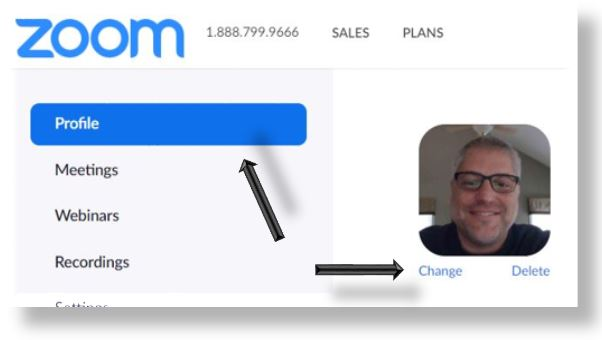
\includegraphics[scale=0.45]{zoom1.jpg}
    \caption{Zoom profile}
    \label{fig:zoom1}
    \end{wrapfigure}
\noindent    
\subsubsection{Profile}
Personalize your profile image! In the desktop application, click the settings (gear icon) button and select \texttt{Profile} $\rightarrow$ \texttt{Edit My Profile}.  If logged into the Zoom website, select \texttt{Profile} from the links on the left and then click the change link beneath your current profile image (see Figure \ref{fig:zoom1}).

\subsubsection{Audio}
It is important to set up your Zoom account so that your audio is muted by default.  There is also an option to that will allow you to enact a push-to-talk. This feature allows you to use your microphone temporarily by pressing and holding a bound-key on your computer (e.g., the spacebar; see Figure \ref{fig:zoom2}).
    \begin{figure}[h]
    \centering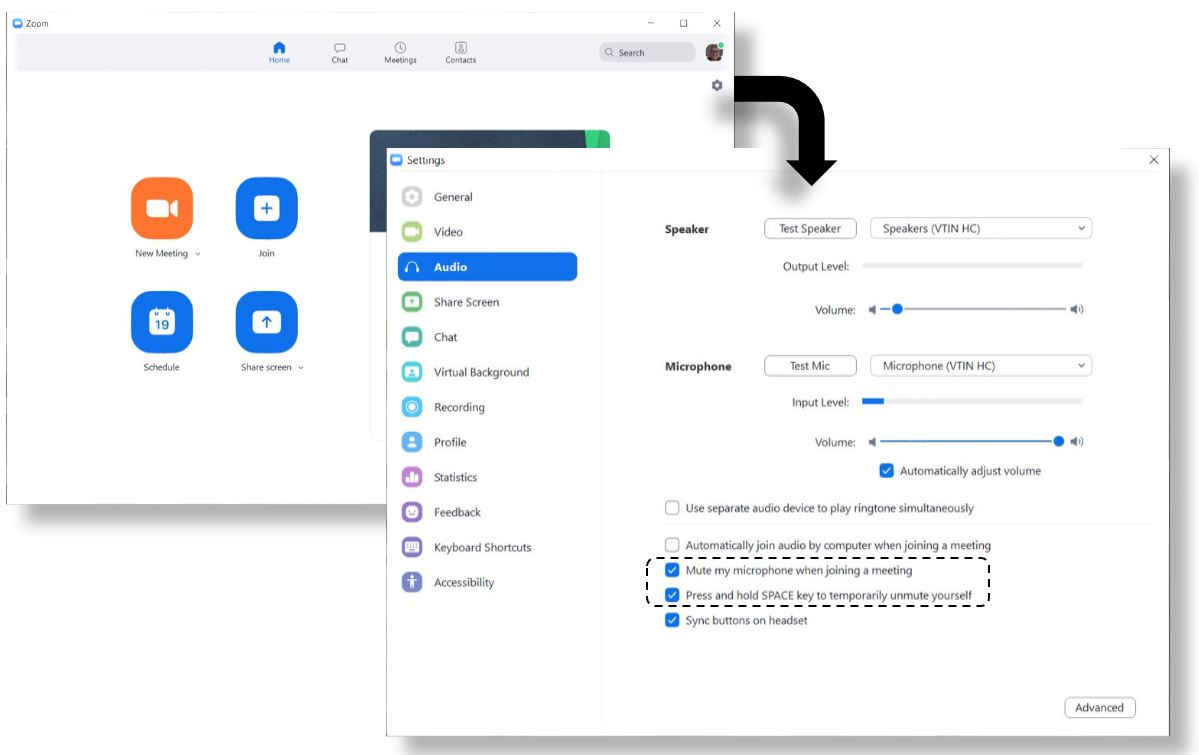
\includegraphics[scale=0.4]{zoomdesktopaudio.jpg}
    \caption{Zoom audio settings}
    \label{fig:zoom2}
    \end{figure}

\subsection{Other Useful Features}
Zoom possesses a number of tools that can facilitate communication in meetings, most of these tools are available to both participants and host(s) of the meetings.  A few of these tools are described below.
\subsubsection{Push-to-Talk}
    Assuming the audio settings are configured as described above, the microphone of all meeting attendees will be muted by default. This is especially helpful in reducing background noise in larger meetings (e.g., >10), which can make it difficult to hear any one speaker in the conversation/presentation.  When an attendee does wish to contribute they can simply hold the space bar down to un-mute the microphone while speaking and release the space bar to re-mute the microphone.
\subsubsection{Screen Sharing}
    Screen sharing is useful for presentations, allowing all participants in the meeting to view the same screen content (e.g., Power Point or Google Slides). Screen sharing can also be configured in settings (gear icon) to display both the shared screen \textit{and} the feed(s) from the participant(s) camera.  There is also a ``whiteboard" option that allows for free form drawing using the cursor or digital pen.    
\subsubsection{Raise Your Hand}
    While Zoom offers a nice interface for large group meetings with a Brady-Bunch style tiling of participants camera feeds, there are cases in which the meeting host might like to present their screen (e.g., f slides) to all participants and may not be aware when there are questions or comments from other participants.  Fortunately, participants (but not hosts) have a ''raise your hand" option when they click the "Participants" button that is part of the Zoom controls when logged into a meeting.  Even when presenting a window in full-screen to participants, the hose will receive an alert when the ''raise your hand" button is clicked by any participant, providing an opportunity to pause the presentation and solicit feedback from meeting participants.
\subsubsection{Annotation Tools}
    Another really useful tool in Zoom is the annotation toolbar.  The toolbar can be made available by clicking the ``Annotate" button in Zoom, whenever the host (or participant) is presenting their screen to the group.  For hosts, the "Spotlight" tool works like a laser pointer that can be used to highlight portions of the screen during a presentation.  Other tools, like "Text" and "Draw" can be useful for participants to make comments or draw attention to a portion of the screen when there are questions during a presentation.  Note, however, that these text and drawing comments are persistent and will need to be erased by the host using the ``Clear" button on the Annotations toolbar when advancing to the next slide (see Figure \ref{fig:zoomannotate}).
    \begin{figure}[h]
    \centering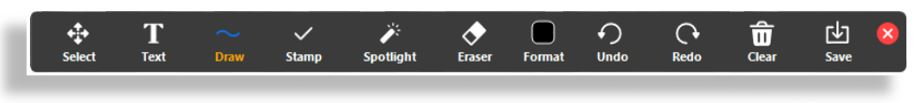
\includegraphics[scale=0.7]{zoomannotate.jpg}
    \caption{Zoom annotation tools}
    \label{fig:zoomannotate}
    \end{figure}
\subsubsection{Chat}
    Zoom also has a ``chat" feature that permits both public and private messaging between participants.  Parameters of the chat permissions are accessible in the ``Chat" panel of the settings (gear icon) menu in Zoom.  Private chats between participants can also be disabled (recommended for webinar/classroom uses).
\subsubsection{Remote Control}
    Remote control is actually one of the "Screen share" options in Zoom. Enabling \texttt{remote control of all operations} can be especially useful in courses that require heavy use of computer applications.  If the situation requires, students can grant you (as the host) control over their computer, meaning that you can use your cursor to control the operation of their computer remotely.  This can be used to demonstrate procedures, install software, etc.
\subsubsection{Scheduling Meetings}
    Meetings can be created ``on the fly" or can be scheduled in advance.  Each meeting is assigned either a unique meeting ID number or your personal meeting ID number (linked to your Zoom account). The meeting ID number determines how participants will access the meeting so an advantage of using your personal ID number is that invited participants will have access the current and any future meeting you host, without the need to repeatedly provide meeting access information (e.g., web links, meeting ID, etc.). You can also set up ``recurring" meetings in Zoom.  Similar to setting up a meeting using your personal ID, these recurring meetings will use a persistent meeting ID number. 
    
    Note that if you configure your recurring Zoom meeting to enable ``join before host", you will effectively have created a persistent virtual meeting room in which participants can interact (even without the meeting host) at any time of day/night.
    

%------------------------------------------------


%\newpage
\newcommand{\SubItem}[1]{
    {\setlength\itemindent{15pt} \item[-] #1}
}

\section{Google Groups}\index{Google Groups}
Google Groups is a great forum for asynchronous communication with students. I find that it is more user friendly than Blackboard's native discussion group features.  When embedded in Blackboard, students can access a course-specific discussion board with just a single click!  Groups are highly configurable, easily searched, and organization of discussions is under the control of the account owner.

In order to set up a Google Group:
\begin{enumerate}
    \item Visit \weblink{https://groups.google.com} and log in with your W\&M credentials.
    \item Click ``Create group"
    \item Enter a name/description for your group and select the options that will determine which features are available in your group (see Figure \ref{fig:googlegroup1}).\\
    \textit{Note: I prefer to use the ``Q\&A forum" option as the format for my class discussion groups because it includes some nice features like allowing students to ``vote" up or down on existing posts/questions and the ability to mark items ``resolved".}
    \begin{figure}[ht]
    \centering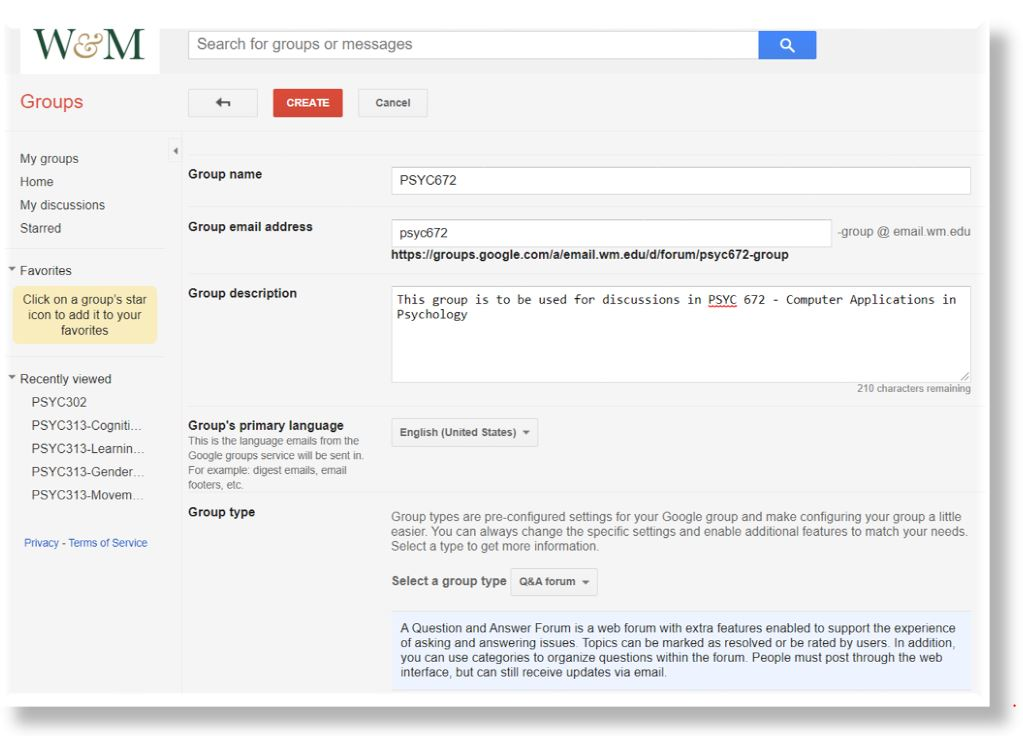
\includegraphics[scale=0.6]{googlegroups1.JPG}
    \caption{Creating a Google Group}
    \label{fig:googlegroup1}
    \end{figure}
    
    \item Scroll down and set your basic visibility and access settings, then click ``Create" to initialize the group.
    \newpage
    \item Get the address of your new group from the address bar in your browser (see Figure \ref{fig:googlegroups2}). You will need this to embed the group in Blackboard.
    \begin{figure}[h]
    \centering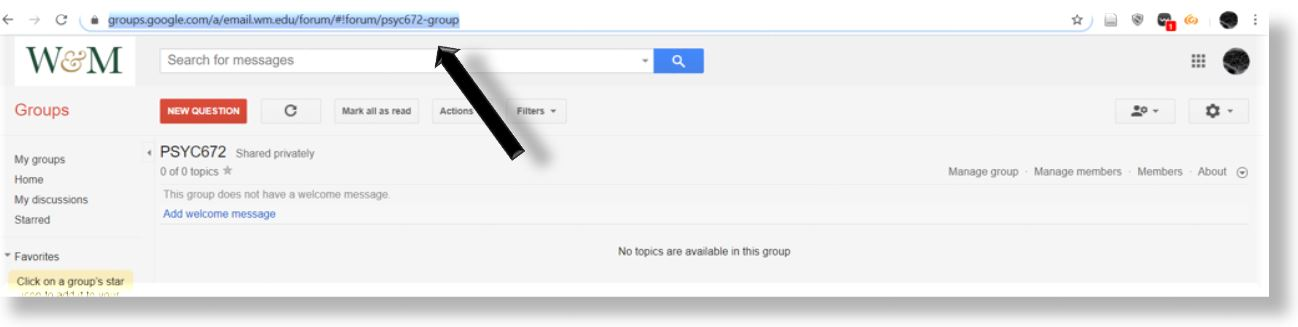
\includegraphics[scale=0.5]{googlegroups2.JPG}
    \caption{A new Google group}
    \label{fig:googlegroups2}
    \end{figure}
    
    \item Embed the group in Blackboard.
    \SubItem If you don't have one already, create a new content area to hold the group.
    \begin{figure}[h]
    \centering
    \centering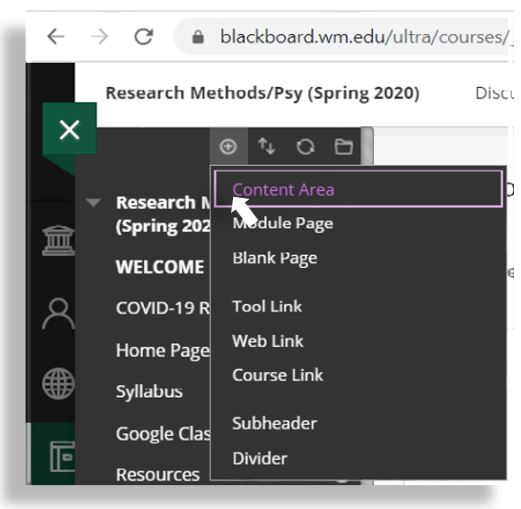
\includegraphics[scale=0.5]{googlegroups3.JPG}
    \caption{Zoom profile}
    \label{fig:googlegroups3}
    \end{figure}
    
    \SubItem Next, add a new ``Item" your content area in Blackboard.
    \begin{figure}[h]
    \centering
    \centering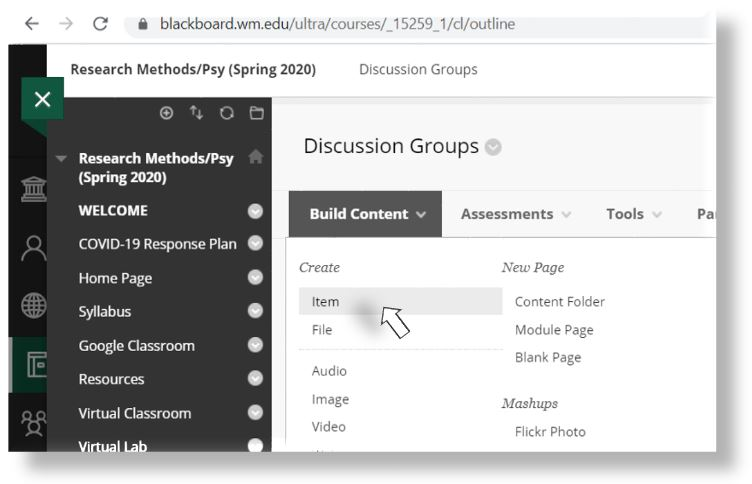
\includegraphics[scale=0.5]{googlegroups4.JPG}
    \caption{Zoom profile}
    \label{fig:googlegroups4}
    \end{figure}
    
    \SubItem Click the ``HTML" button in the text editor panel (see Figure \ref{fig:googlegroups5}) to open the HTML window.
    \begin{figure}[h]
    \centering
    \centering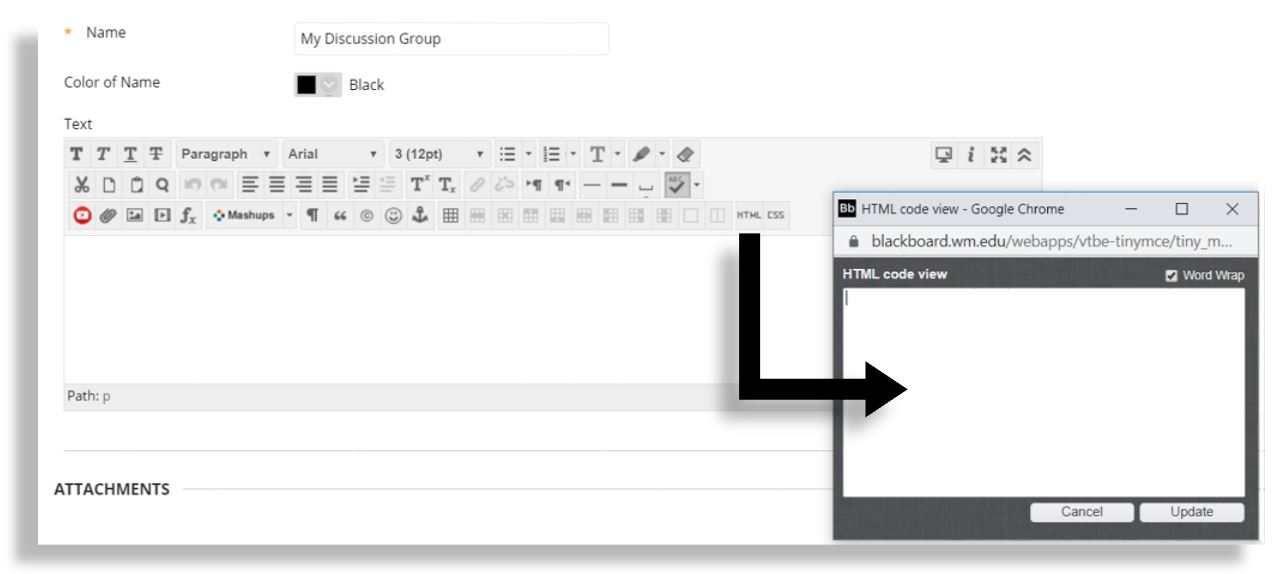
\includegraphics[scale=0.5]{googlegroups5.JPG}
    \caption{Embedding the group}
    \label{fig:googlegroups5}
    \end{figure}
    
    \SubItem Now go to your Google Groups group page and click the settings (gear icon) button and select ``group settings".
    
    \SubItem Scroll down until you see ``Embedding your group", then copy the embed code provided for you. 

    \SubItem Paste the code you just copied into the HTML window in Blackboard and click the ``Update" button. A yellow box will appear in the text panel of the Blackboard item.  Click the ``Submit" button to complete the process.
\end{enumerate} 
\vspace{.5cm}

Once these steps are completed, your students will be able to access the discussion board with a single click on the Content Area in Blackboard.  Students can easily post a new question, or search/filter existing posts for answers to previously posted questions (see Figure \ref{fig:googlegroups6}).
    \begin{figure}[h]
    \centering
    \centering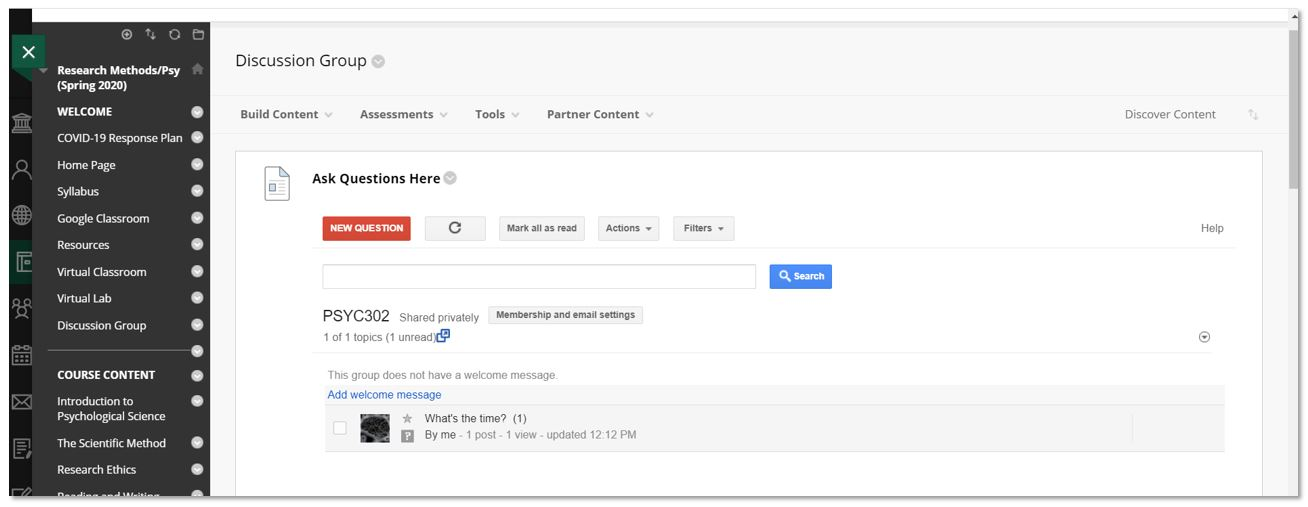
\includegraphics[scale=0.55]{googlegroups6.JPG}
    \caption{Google Group embedded in Blackboard}
    \label{fig:googlegroups6}
    \end{figure}
%\begin{lstlisting}[language=HTML,basicstyle=\footnotesize]


%----------------------------------------------------------------------------------------
%	BIBLIOGRAPHY
%----------------------------------------------------------------------------------------
\printglossary[style=twocolumn]
\bibliography{bibliography}
%\chapter*{Bibliography}
%\addcontentsline{toc}{chapter}{\textcolor{ocre}{Bibliography}} % Add a Bibliography heading to the table of contents

%------------------------------------------------

%\section*{Articles}
%\addcontentsline{toc}{section}{Articles}
%\printbibliography[heading=bibempty,type=article]

%------------------------------------------------

%\section*{Books}
%\addcontentsline{toc}{section}{Books}
%\printbibliography[heading=bibempty,type=book]

%----------------------------------------------------------------------------------------
%	INDEX
%----------------------------------------------------------------------------------------

\cleardoublepage % Make sure the index starts on an odd (right side) page
\phantomsection
\setlength{\columnsep}{0.75cm} % Space between the 2 columns of the index
\addcontentsline{toc}{chapter}{\textcolor{ocre}{Index}} % Add an Index heading to the table of contents
\printindex % Output the index

%----------------------------------------------------------------------------------------

\end{document}
